\section*{第八章 概率与统计}

\section*{一、概率初步、统计}

\section*{【典型题型和解题技巧】}

例 1 某大学为了支援教育事业, 决定从 2024 年应届毕业生报名的 18 名志愿者中, 选取 6 人组成志愿小组赴宁夏支教. 试设计两种抽样方案.

解 (抽签法) 先将 18 名志愿者编号为 01,02,03, $\cdots ,{18}$ ,并将这 18 个号码写在形状、大小相同的号签上(号签可以用小球、卡片、纸片等制作),然后将这 18 个号签放入一个不透明的盒子里,充分 “搅拌均匀”,从盒子中逐个抽取 6 个号签,并记录上面的编号,所得号码对应的志愿者, 就是志愿小组的成员.

(随机数表法) 第一步:将 18 名志愿者编号,编号为 01,02,03, $\cdots ,{18}$ ；

第二步:在随机数表中任选一个随机数开始读, 按任意方向读数, 比如向右读;

第三步:每次取两位,凡不在 01\~18 中的数,或已读过的数,都跳过去不做记录,直到选取 6 个满足条件的号码;

第四步:找出以上号码对应的志愿者,就是志愿小组的成员.

注意 当总体中的个体数较少时, 一般采用简单随机抽样, 常用的简单随机抽样方法有两种:抽签法和随机数表法. 抽签法的操作步骤是:编号→制签→搅匀→抽取,而随机数表法的操作步骤是:编号→确定起始数 $\rightarrow$ 确定读数方向→取得样本.

例 2 若某袋中有 5 个大小、质地完全相同的球, 其中有 2 个红球、 3 个黄球, 从中不放回地依次随机摸出 2 个球,记事件 $A =$ “第一次摸到红球”,事件 $B =$ “第二次摸到红球”.

(1)求 $P\left( A\right)$ 和 $P\left( B\right)$ 的值；

( 2 )求两次摸到的不都是红球的概率.

解(1)将两个红球编号为 1,2,三个黄球编号为 3,4,5.

第一次摸球时有 5 种等可能的结果;

对应第一次摸球的每个可能结果,

第二次摸球时有 4 种等可能的结果.

将两次摸球的结果配对, 组成 20 种等可能的结果,

第一次摸到红球的可能结果有 8 种,即

$A = \{ \left( {1,2}\right) ,\left( {1,3}\right) ,\left( {1,4}\right) ,\left( {1,5}\right) ,\left( {2,1}\right) ,\left( {2,3}\right) ,\left( {2,4}\right) ,\left( {2,5}\right) \}$ ,所以 $P\left( A\right)  = \dfrac{8}{20} = \dfrac{2}{5}$ .

第二次摸到红球的可能结果也有 8 种, 即

$B = \{ \left( {2,1}\right) ,\left( {3,1}\right) ,\left( {4,1}\right) ,\left( {5,1}\right) ,\left( {1,2}\right) ,\left( {3,2}\right) ,\left( {4,2}\right) ,\left( {5,2}\right) \}$ ,所以 $P\left( B\right)  = \dfrac{8}{20} = \dfrac{2}{5}$ .

(2)事件 $A \cap  B$ 表示“两次摸到都是红球”包含 2 个可能结果,即 $A \cap  B = \{ \left( {1,2}\right) ,\left( {2,1}\right) \}$ ,

则两次摸到都是红球的概率 $P\left( {A \cap  B}\right)  = \dfrac{2}{20} = \dfrac{1}{10}$ ,

故两次摸到的不都是红球的概率 $P\left( {\bar{A} \cup  \bar{B}}\right)  = 1 - P\left( {A \cap  B}\right)  = 1 - \dfrac{1}{10} = \dfrac{9}{10}$ .

注意 当某一事件的概率不易求出或求解比较麻烦, 但其对立事件的概率容易求得时, 可先求其对立事件的概率.

例 3 在信道内传输 0,1 信号,信号的传输相互独立. 发送 0 时,收到 1 的概率为 $\dfrac{1}{2}$ ,收到 0 的概率为 $\dfrac{1}{2}$ ; 发送 1 时,收到 0 的概率为 $\dfrac{1}{3}$ ,收到 1 的概率为 $\dfrac{2}{3}$ .

(1)重复发送信号 1 三次,计算至少收到两次 1 的概率；

(2)依次发送1,1,0,记事件 $A$ :至少收到一个正确信号；②事件 $B$ :至少收到两个 0 . 这 2 个事件是否互相独立? 请证明.

解(1)重复发送信号 1 三次,“至少收到两次 1 ”的可能情况为: $\left( {1,1,1}\right) ,\left( {1,0,1}\right) ,(1,1$ , $0),\left( {0,1,1}\right)$ ,因为信号的传输相互独立,故“至少收到两次 1 ”的概率为: $\dfrac{2}{3} \times  \dfrac{2}{3} \times  \dfrac{2}{3} + \dfrac{2}{3} \times  \dfrac{1}{3} \times$  $\dfrac{2}{3} + \dfrac{2}{3} \times  \dfrac{2}{3} \times  \dfrac{1}{3} + \dfrac{1}{3} \times  \dfrac{2}{3} \times  \dfrac{2}{3} = \dfrac{20}{27}.$

(2)事件 $A$ 与事件 $B$ 不互相独立,证明如下:

若依次发送1,1,0,则三次都没收到正确信号的概率为 $\dfrac{1}{3} \times  \dfrac{1}{3} \times  \dfrac{1}{2} = \dfrac{1}{18}$ ,故至少收到一个正确信号的概率为 $P\left( A\right)  = 1 - \dfrac{1}{18} = \dfrac{17}{18}$ ;

若依次发送 1,1,0,“至少收到两个 0”的可能情况为: $\left( {0,0,0}\right) ,\left( {0,0,1}\right) ,\left( {0,1,0}\right) ,\left( {1,0,0}\right)$ , 故 $P\left( B\right)  = \dfrac{1}{3} \times  \dfrac{1}{3} \times  \dfrac{1}{2} + \dfrac{1}{3} \times  \dfrac{1}{3} \times  \dfrac{1}{2} + \dfrac{1}{3} \times  \dfrac{2}{3} \times  \dfrac{1}{2} + \dfrac{2}{3} \times  \dfrac{1}{3} \times  \dfrac{1}{2} = \dfrac{6}{18} = \dfrac{1}{3}$ .

若依次发送 1,1,0,“至少收到两个 0 且至少收到一个正确信号”的可能情况为:

$\left( {0,0,0}\right) ,\left( {0,1,0}\right) ,\left( {1,0,0}\right)$ ,故 $P\left( {A \cap  B}\right)  = \dfrac{1}{3} \times  \dfrac{1}{3} \times  \dfrac{1}{2} + \dfrac{1}{3} \times  \dfrac{2}{3} \times  \dfrac{1}{2} + \dfrac{2}{3} \times  \dfrac{1}{3} \times  \dfrac{1}{2} = \dfrac{5}{18}$ .

因为 $P\left( A\right) P\left( B\right)  \neq  P\left( {A \cap  B}\right)$ ,所以事件 $A$ 与事件 $B$ 不互相独立.

注意 $P\left( {A \cap  B}\right)  = P\left( A\right) P\left( B\right)$ 是事件 $A,B$ 相互独立的严格定义,在此基础上,可以证明若事件 $A,B$ 独立,则事件 $A$ 与 $\bar{B}$ ,事件 $\bar{A}$ 与 $B$ ,事件 $\bar{A}$ 与 $\bar{B}$ 也独立. 值得一提的是,对于三个事件 $A,B,C$ 而言,“事件 $A,B,C$ 相互独立”与“事件 $A,B,C$ 两两独立”是不同的,其中一个著名的案例是伯恩斯坦反例,有兴趣的同学可以参阅大学数学概率统计教材.

例 4 某校对全校高二学生进行数学测试, 并从中随机抽取了 100 名学生的成绩, 被抽取的成绩全部介于 40 分到 100 分之间 (满分 100 分), 将统计结果按照如下方式分成六组: 第一组 $\lbrack {40},{50})$ ,第二组 $\lbrack {50},{60}),\cdots$ ,第六组 $\left\lbrack  {{90},{100}}\right\rbrack$ ,画出频率分布直方图如图 1 所示.

(1)求频率分布直方图中 $a$ 的值；

\begin{center}
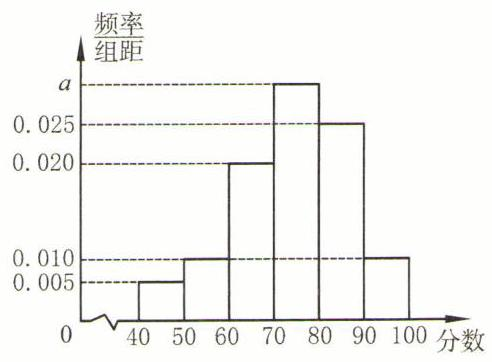
\includegraphics[width=0.4\textwidth]{bodyxb/src/bo_d20aucref24c73anc48g_241_954_196_492_362_0.jpg}
\end{center}


(图 1)

(2)求该样本的中位数；

(3)为进一步了解学生的学习情况,从分数位于 $\lbrack {50},{80})$ 的学生中,按照第二组,第三组,第四组分层抽样 6 人,再从 6 人中任取 2 人,求此 2 人分属不同组的概率.

解(1)由频率分布直方图可得(0.005+0.01+0.02 $+ {0.025} + a + {0.01}) \times  {10} = 1$ ,得 $a = {0.03}$ .

(2)设该样本的中位数为 $x$ ,所以 ${0.05} + {0.1} + {0.2} +$  $\dfrac{{0.3}\left( {x - {70}}\right) }{10} = {0.5}$ ,得 $x = {75}$ .

(3)由分层抽样知,第二组中抽 1 人,记作 $a$ ,第三组中抽 2 人,记作 ${b}_{1}$ , ${b}_{2}$ ,第四组中抽 3 人,记作 ${c}_{1},{c}_{2},{c}_{3}$ ,这 6 人中抽取 2 人有 $\left( {a,{b}_{1}}\right) ,\left( {a,{b}_{2}}\right) ,\left( {a,{c}_{1}}\right) ,\left( {a,{c}_{2}}\right) ,\left( {a,{c}_{3}}\right) ,\left( {{b}_{1},{b}_{2}}\right)$ , $\left( {{b}_{1},{c}_{1}}\right) ,\left( {{b}_{1},{c}_{2}}\right) ,\left( {{b}_{1},{c}_{3}}\right) ,\left( {{b}_{2},{c}_{1}}\right) ,\left( {{b}_{2},{c}_{2}}\right) ,\left( {{b}_{2},{c}_{3}}\right) ,\left( {{c}_{1},{c}_{2}}\right) ,\left( {{c}_{1},{c}_{3}}\right) ,\left( {{c}_{2},{c}_{3}}\right)$ ,共 15 个样本点; 2 人来自同一组的有 $\left( {{b}_{1},{b}_{2}}\right) ,\left( {{c}_{1},{c}_{2}}\right) ,\left( {{c}_{1},{c}_{3}}\right) ,\left( {{c}_{2},{c}_{3}}\right)$ ,共 4 个样本点,所以 2 人来自不同组的概率 $p = 1 - \dfrac{4}{15} = \dfrac{11}{15}$ .

注意 需要指出的是,利用分层抽样抽取第 $i$ 层个体数目 ${n}_{i}$ 的时候,可能会遇到个体数目 ${n}_{i}$ 不是整数的情形,对此,一个较为常见的处理方式是: 通过四舍五入取 ${n}_{i}$ 的近似值,且保证各 ${n}_{i}$ 之和等于样本容量 $n$ 即可.

例 5 用分层随机抽样从某校高一年级学生的数学期末成绩(满分 100 分,成绩都是整数)中抽取一个容量为 100 的样本,其中男生成绩数据 40 个,女生成绩数据 60 个,再将 40 个男生成绩样本数据分为 6 组: $\lbrack {40},{50})$ , $\lbrack {50},{60}),\lbrack {60},{70}),\lbrack {70},{80}),\lbrack {80},{90}),\left\lbrack  {{90},{100}}\right\rbrack$ . 绘制得到如图 2 所示的频率分布直方图.

\begin{center}
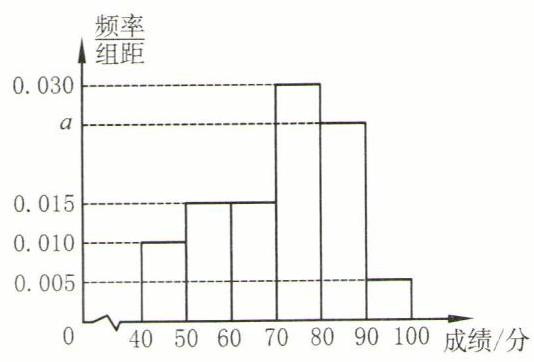
\includegraphics[width=0.4\textwidth]{bodyxb/src/bo_d20aucref24c73anc48g_241_913_1241_534_362_0.jpg}
\end{center}


(图 2)

(1)求 $a$ 的值；

(2)若在区间 $\lbrack {40},{50})$ 和 $\left\lbrack  {{90},{100}}\right\rbrack$ 内的两组男生成绩样本数据中,随机抽取 2 个进行调查,求调查对象来自不同分组的概率；

(3)已知男生成绩样本数据的平均数和方差分别为 71 和 187.75,女生成绩样本数据的平均数和方差分别为 73.5 和 119 ,求总样本的平均数和方差.

解 (1) 由题意得 $\left( {{0.010} + {0.015} + {0.015} + {0.030} + a + {0.005}}\right)  \times  {10} = 1$ ,解得 $a = {0.025}$ .

(2) ${0.010} \times  {10} \times  {40} = 4,{0.005} \times  {10} \times  {40} = 2$ ,所以成绩在区间 $\lbrack {40},{50})$ 的男生有 4 人,在区间 $\left\lbrack  {{90},{100}}\right\rbrack$ 的男生有 2 人.

设成绩在区间 $\lbrack {40},{50})$ 的男生为 $a,b,c,d$ ,在区间 $\left\lbrack  {{90},{100}}\right\rbrack$ 的男生为 $m,n$ ,则在这 6 个数据中随机抽取 2 个的样本空间 $\Omega$ 包含的样本点为: ${ab},{ac},{ad},{am},{an},{bc},{bd},{bm},{bn},{cd},{cm}$ , ${cn},{dm},{dn},{mn}$ ,所以 $\left| \Omega \right|  = {15}$ .

记事件 $A =$ “调查对象来自不同分组”,则事件 $A$ 包含的样本点为 ${am},{an},{bm},{bn},{cn},{cn}$ , ${dm},{dn},\left| A\right|  = 8$ ,所以调查对象来自不同的分组的概率为 $P\left( A\right)  = \dfrac{\left| A\right| }{\left| \Omega \right| } = \dfrac{8}{15}$ .

(3)设男生成绩样本数据为 ${x}_{1},{x}_{2},\cdots ,{x}_{40}$ ,其平均数为 $\bar{x} = {71}$ ,方差为 ${s}_{x}^{2} = {187.75}$ ,

女生成绩样本数据为 ${y}_{1},{y}_{2},\cdots ,{y}_{60}$ ,其平均数为 $\bar{y} = {73.5}$ ,方差为 ${s}_{y}^{2} = {119}$ .

设总体的平均数为 $\bar{z}$ ,方差为 ${s}^{2}$ ,由分层抽样总体样本平均数与各层样本平均数的关系得 $\bar{z} = \dfrac{40}{100}\bar{x} + \dfrac{60}{100}\bar{y} = {72.5},$

因为 ${s}^{2} = \dfrac{1}{100}\left\lbrack  {\mathop{\sum }\limits_{{i = 1}}^{{40}}{\left( {x}_{i} - \bar{z}\right) }^{2} + \mathop{\sum }\limits_{{i = 1}}^{{60}}{\left( {y}_{i} - \bar{z}\right) }^{2}}\right\rbrack   = \dfrac{1}{100}\left\lbrack  {\mathop{\sum }\limits_{{i = 1}}^{{40}}{\left( {x}_{i} - \bar{x} + \bar{x} - \bar{z}\right) }^{2} + \mathop{\sum }\limits_{{i = 1}}^{{60}}{\left( {y}_{i} - \bar{y} + \bar{y} - \bar{z}\right) }^{2}}\right\rbrack$ ,

$\mathop{\sum }\limits_{{i = 1}}^{{40}}2\left( {{x}_{i} - \bar{x}}\right) \left( {\bar{x} - \bar{z}}\right)  = 2\left( {\bar{x} - \bar{z}}\right) \mathop{\sum }\limits_{{i = 1}}^{{40}}\left( {{x}_{i} - \bar{x}}\right)  = 2\left( {\bar{x} - \bar{z}}\right) \left( {\mathop{\sum }\limits_{{i = 1}}^{{40}}{x}_{i} - {40}\bar{x}}\right)  = 0,$

同理 $\mathop{\sum }\limits_{{i = 1}}^{{60}}2\left( {{y}_{i} - \bar{y}}\right) \left( {\bar{y} - \bar{z}}\right)  = 0$ ,

所以 ${s}^{2} = \dfrac{1}{100}\left\lbrack  {\mathop{\sum }\limits_{{i = 1}}^{{10}}{\left( {x}_{i} - \bar{x}\right) }^{2} + \mathop{\sum }\limits_{{i = 1}}^{{40}}{\left( \bar{x} - \bar{z}\right) }^{2} + \mathop{\sum }\limits_{{i = 1}}^{{60}}{\left( {y}_{i} - \bar{y}\right) }^{2} + \mathop{\sum }\limits_{{i = 1}}^{{60}}{\left( \bar{y} - \bar{z}\right) }^{2}}\right\rbrack$

$= \dfrac{1}{100}\left\lbrack  {{40}{s}_{x}^{2} + {40}{\left( \bar{x} - \bar{z}\right) }^{2} + {60}{s}_{y}^{2} + {60}{\left( \bar{y} - \bar{z}\right) }^{2}}\right\rbrack$

$= \dfrac{1}{100}\left\lbrack  {{40} \times  {187.75} + {40} \times  {\left( {71} - {72.5}\right) }^{2} + {60} \times  {119} + {60} \times  {\left( {73.5} - {72.5}\right) }^{2}}\right\rbrack$

$= {148},$

所以总样本的平均数和方差分别为 72.5 和 148.

注意 总样本平均数与方差的结果都不依赖于男生、女生的样本量,而只依赖于两个样本量之比.

\section*{【训练题】}

\section*{(A)}

1. 用随机数表法进行抽样有以下几个步骤:①将总体中的个体编号；②获取样本号码；③选定开始的数字；④选定读数的方向. 这些步骤的先后顺序应为(   )

(A) ②①③④. (B) ③④①②. (C) ①③④②. (D) ④①③②.

2. 某教育部门为调查中小学生每日完成作业的时间,收集了某位学生 100 天每天完成作业的时间, 并绘制了如图所示的频率分布直方图(每个区间均为左闭右开),根据此直方图得出了下列结论, 其中正确的是(   )

\begin{center}
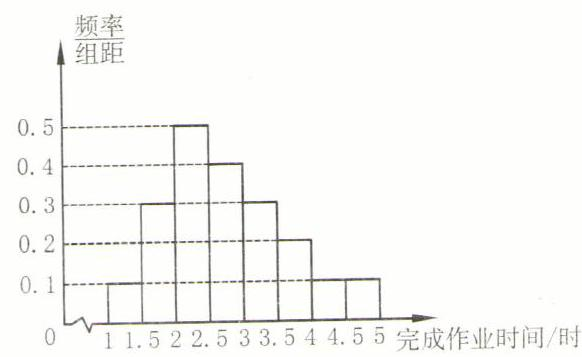
\includegraphics[width=0.4\textwidth]{bodyxb/src/bo_d20aucref24c73anc48g_242_941_1790_582_357_0.jpg}
\end{center}


(第 2 题)

(A)估计该学生每日完成作业的时间在 2 小时至 2.5 小时的有 50 天.

(B) 估计该学生每日完成作业时间超过 3 小时的概率为 0.3 .

(C) 估计该学生每日完成作业时间的中位数为 2.625 小时.

(D) 估计该学生每日完成作业时间的众数为 2.3 小时.

3. 2016 年至 2023 年我国原油进口数量如图所示:

${\Delta 13.6}\% {\Delta 10.1}\% {\Delta 10.1}\% {\Delta 9.5}\% {\Delta 7.3}\% \nabla  - {5.4}\% \nabla  - {0.9}\% {\Delta 11}\%$

\begin{center}
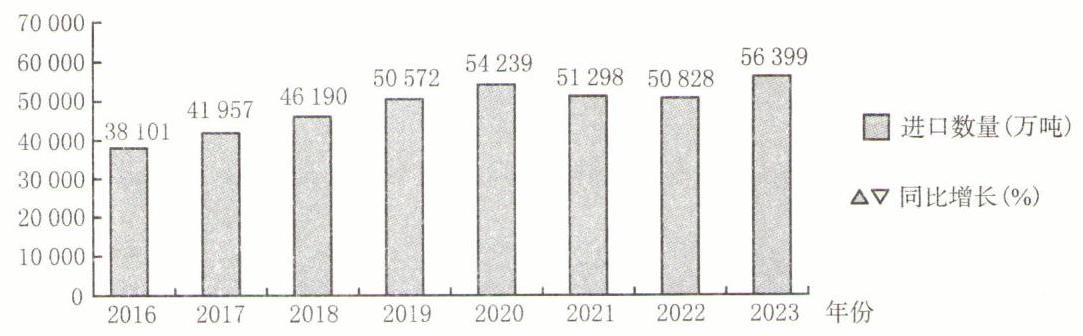
\includegraphics[width=0.9\textwidth]{bodyxb/src/bo_d20aucref24c73anc48g_243_242_401_1083_336_0.jpg}
\end{center}


(第 3 题)

下列结论正确的是(   )

(A)2016 年至 2023 年我国原油进口数量逐年增加.

(B) 2016 年至 2023 年我国原油进口数量的极差为 16138 万吨.

(C) 2016 年至 2023 年我国原油进口数量的第 80 百分位数为 54239 万吨.

(D) 2015 年我国原油进口数量少于 30000 万吨.

4. 已知事件 $A,B$ 满足 $P\left( A\right)  = \dfrac{1}{3},P\left( B\right)  = \dfrac{1}{2}$ ,则下列选项错误的是 (   )

(A) 若 $A,B$ 互斥,则 $P\left( {A \cap  B}\right)  = \dfrac{1}{6}$ .

(B) 若 $A,B$ 互斥,则 $P\left( {A \cup  \bar{B}}\right)  = \dfrac{1}{2}$ .

(C) 若 $A,B$ 独立,则 $P\left( {A \cap  \bar{B}}\right)  = \dfrac{1}{6}$ .

(D) 若 $A,B$ 独立,则 $P\left( {A \cup  B}\right)  = \dfrac{2}{3}$ .

5. 口袋中装有除颜色外其他完全相同的 3 个红球、 2 个白球和 1 个黄球,从中任取一个球,事件 $A$ 表示 “取到的是红球”,事件 $B$ 表示 “取到的是白球”,事件 $C$ 表示 “取到的是黄球”, 则(   )

(A) $P\left( {A \cup  B}\right)  = 1$ . (B) 事件 $A,B,C$ 可能同时发生.

(C) $\bar{A}$ 与 $\bar{B}$ 互斥. (D) 事件 $A$ 与事件 $B$ 不相互独立.

6. 一个袋子中有标号分别为1,2,3,4的 4 个球,除标号外没有其他差异. 采用不放回方式从中任意摸球两次,设事件 $A =$ “第一次摸出球的标号小于 ${3}^{n}$ ,事件 $B =$ ”第二次摸出球的标号小于 3 ”,事件 $C =$ “第一次摸出球的标号为奇数”,则(   )

(A) $A$ 与 $B$ 互斥. (B) $A$ 与 $B$ 相互独立.

(C) $A$ 与 $C$ 互斥. (D) $A$ 与 $C$ 相互独立.

7. 如图,电路中 $A,B,C$ 三个电子元件正常工作的概率分别为 $P\left( A\right)  = \dfrac{1}{3}$ , $P\left( B\right)  = \dfrac{1}{2},P\left( C\right)  = \dfrac{3}{5}$ ,则该电路正常工作的概率为 (   )

\begin{center}
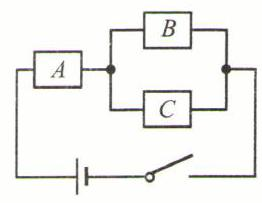
\includegraphics[width=0.2\textwidth]{bodyxb/src/bo_d20aucref24c73anc48g_244_1246_140_262_203_0.jpg}
\end{center}


(第 7 题)

(A) $\dfrac{4}{15}$ . (B) $\dfrac{8}{15}$ .

(C) $\dfrac{7}{15}$ . (D) $\dfrac{7}{12}$ .

8. 若 $P\left( {A \cap  B}\right)  = \dfrac{1}{10},P\left( \bar{A}\right)  = \dfrac{3}{5},P\left( B\right)  = \dfrac{1}{4}$ ,则 (   )

(A) 事件 $A$ 与 $B$ 互斥. (B) 事件 $A$ 与 $B$ 相互独立.

(C) $P\left( {A \cup  B}\right)  = \dfrac{13}{20}$ . (D) $P\left( {\bar{A} \cap  B}\right)  = \dfrac{1}{5}$ .

9. 在某学校开展的“防电信诈骗知识竞赛”活动中,高三年级派出甲、乙、丙、丁四个小组参赛, 每个小组各有 10 位选手. 记录参赛人员失分 (均为非负整数) 情况, 若小组的每位选手失分都不超过 7 分,则该组为 “优秀小组”. 已知选手失分数据信息如下,则一定为 “优秀小组” 的是(   )

(A) 甲组中位数为 3 , 极差为 5 . (B) 乙组平均数为 2 , 众数为 2 .

(C) 丙组平均数为 2 , 方差为 3 . (D) 丁组平均数为 2, 第 85 百分位数为 7 .

10. 已知样本数据 ${x}_{1},{x}_{2},\cdots ,{x}_{9}$ 的平均数为 9,方差为 12,现这组样本数据增加一个数据 ${x}_{10}$ , 此时新样本数据的平均数为 10 ,则新样本数据的方差为 (   )

(A) 18.2 . (B) 19.6. (C) 19.8. (D) 21.7.

11. 已知数据 ${x}_{1},{x}_{2},\cdots ,{x}_{5}$ 的平均数为 4,方差为 2,数据 ${y}_{1},{y}_{2},\cdots ,{y}_{5}$ 的平均数为 2,方差为 4. 若将这两组数据混合形成一组新的数据,则新的这组数据的方差为(   )

(A) 6. (B) 2. (C) 3. (D) 4.

12. 某学校高三年级男生共有 ${N}_{1}$ 个,女生共有 ${N}_{2}$ 个,为调查该年级学生的年龄情况,通过分层抽样,得到男生和女生样本数据的平均数和方差分别为 $\overline{{x}_{1}},\overline{{x}_{2}}$ 和 ${s}_{1}^{2},{s}_{2}^{2}$ . 已知 $\overline{{x}_{1}} = \overline{{x}_{2}}$ ,则该校高三年级全体学生年龄的方差为(   )

(A) ${N}_{1}{s}_{1}^{2} + {N}_{2}{s}_{2}^{2}$ . (B) ${N}_{2}{s}_{1}^{2} + {N}_{1}{s}_{2}^{2}$ .

(C) $\dfrac{{N}_{1}}{{N}_{1} + {N}_{2}}{s}_{1}^{2} + \dfrac{{N}_{2}}{{N}_{1} + {N}_{2}}{s}_{2}^{2}$ . (D) $\dfrac{{N}_{2}}{{N}_{1} + {N}_{2}}{s}_{1}^{2} + \dfrac{{N}_{1}}{{N}_{1} + {N}_{2}}{s}_{2}^{2}$ .

13. 某同学统计最近 5 次考试成绩, 发现分数恰好组成一个公差不为 0 的等差数列, 设 5 次成绩的平均数为 $\bar{x}$ ,第 60 百分位数为 $m$ ,当去掉某一次的成绩后,4次成绩的平均数为 $\bar{y}$ ,第 60 百分位数为 $n$ . 若 $\bar{y} = \bar{x}$ ,则 (   )

(A) $m > n$ . (B) $m = n$ .

(C) $m < n$ . (D) $m$ 与 $n$ 大小无法判断.

14. 已知样本数据0,1,2,3,4,5,6,7,8,9的第 25 百分位数为 $a$ ,第 75 百分位数为 $b$ ,从样本数据落在区间 $\left\lbrack  {0,a}\right\rbrack  ,\left( {a,b}\right) ,\left\lbrack  {b,9}\right\rbrack$ 内的数据中各取一个数组成一个三位数,则所组成的三位数中能被 3 整除的个数为(   )

(A) 54. (B) 60. (C) 64. (D) 72.

15. 某地区为了解最近 11 天该地区的空气质量,调查了该地区过去 11 天小颗粒物的浓度(单位: $\mu \mathrm{g}/{\mathrm{m}}^{3}$ ),数据依次为 ${53},{56},{69},{70},{72},{79},{65},{80},{45},{41},m\left( {m > {50}}\right)$ . 已知这组数据的极差为 40,则这组数据的第 $m$ 百分位数为\blkda{}.

16. 设实数 $x,y\left( {4 \leq  x < y}\right)$ 满足 $1,3,4,x,y,y + 2$ 的平均数与第 50 百分位数相等,则数据 $x$ , $y,y + 2$ 的方差为\blkda{}.

17. 为获得某中学高一学生的身高(单位:cm)信息,采用随机抽样方法抽取了样本量为 50 的样本, 其中男、女生样本量均为 25 , 计算得到男生样本的均值为 176 , 标准差为 10 , 女生样本的均值为 166 ,标准差为 20 . 则总样本的方差为\blkda{} ${\mathrm{{cm}}}^{2}$ .

18. 一个盒子中装有 4 张卡片,卡片上分别写有数字 1,2,3,4 . 现从盒子中随机抽取卡片.

(1)若一次抽取 3 张卡片,事件 $A$ 表示 “ 3 张卡片上数字之和大于 7 ”,求 $P\left( A\right)$ ；

(2)若第一次抽取 1 张卡片,放回后再抽取 1 张卡片,事件 $B$ 表示 “两次抽取的卡片上数字之和大于 6 ”,求 $P\left( B\right)$ ；

(3)若一次抽取 2 张卡片,事件 $C$ 表示 “ 2 张卡片上数字之和是 3 的倍数”,事件 $D$ 表示 “ 2 张卡片上数字之积是 4 的倍数”,验证 $C,D$ 是独立的.

19. 有人说: “如果抽样方法设计得好, 对 243 名学生进行视力调查与对 24300 名学生进行视力普查的结果会差不多,而且对于教育部门掌握学生视力状况来说,因为节省了人力、物力,抽样调查更可取. ”你认为这种说法有道理吗? 为什么?

20. 文明城市是反映城市整体文明水平的综合性荣誉称号,作为普通市民,既是文明城市的最大受益者, 更是文明城市的主要创造者. 某市为提高市民对文明城市创建的认识,举办了“创建文明城市知识竞赛”, 从所有答卷中随机抽取 100 份作为样本, 将样本的成绩(满分 100 分,成绩均为不低于 40 分的整数)分成六段: $\lbrack {40},{50}),\lbrack {50},{60}),\cdots ,\left\lbrack  {{90},{100}}\right\rbrack$ . 得到如图所示的频率分布直方图.

\begin{center}
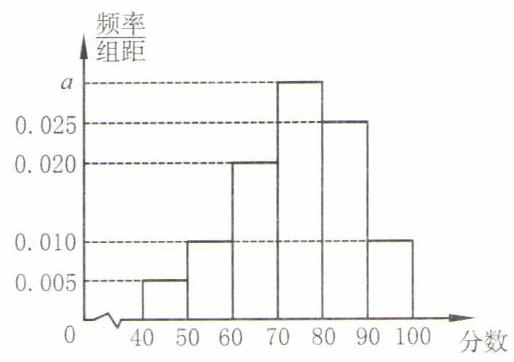
\includegraphics[width=0.4\textwidth]{bodyxb/src/bo_d20aucref24c73anc48g_245_926_1220_514_362_0.jpg}
\end{center}


(第 20 题)

(1)求频率分布直方图中 $a$ 的值；

(2)试估计该样本成绩的第 75 百分位数；

(3)已知落在 $\lbrack {50},{60})$ 的平均成绩是 57,方差是 7,落在 $\lbrack {60},{70})$ 的平均成绩为 69,方差是 4,求两组成绩的总平均数 $\bar{z}$ 和总方差 ${s}^{2}$ .

21. 近年来, “直播带货”受到越来越多人的喜爱, 目前已经成为推动消费的一种流行营销形式. 某直播平台有 1000 个直播商家, 对其进行调查统计, 发现所售商品多为小吃、衣帽、生鲜、玩具、饰品类等,各类直播商家所占比例如图 1 所示. 为了更好地服务买卖双方,该直播平台打算用分层抽样的方式抽取 80 个直播商家进行问询交流.

(1)应抽取小吃类、生鲜类商家各多少家?

(2)在问询了解直播商家的利润状况时,工作人员对抽取的 80 个商家的平均日利润进行了统计 (单位:元), 所得频率分布直方图如图 2 所示.

①估计该直播平台商家平均日利润的第 75 百分位数；

②若将平均日利润超过 480 元的商家称为 “优质商家”,估计该直播平台 “优质商家” 的个数.

\begin{center}
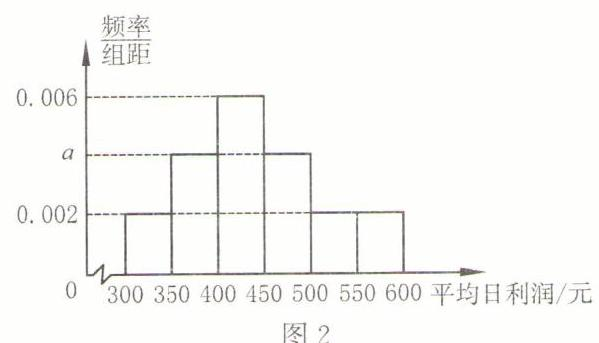
\includegraphics[width=0.5\textwidth]{bodyxb/src/bo_d20aucref24c73anc48g_246_770_421_599_343_0.jpg}
\end{center}


\begin{center}
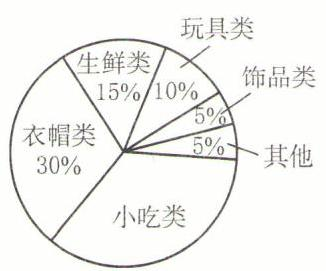
\includegraphics[width=0.2\textwidth]{bodyxb/src/bo_d20aucref24c73anc48g_246_305_465_326_271_0.jpg}
\end{center}


图 1

(第 21 题)

22. 某中学为了调查高一年级学生劳动实践活动情况, 对 500 名学生某周的劳动时间统计如下:

\begin{center}
\adjustbox{width=\textwidth}{
\begin{tabular}{|c|c|c|c|c|c|}
\hline
周劳动时间/时 & $\lbrack 1,2)$ & $\lbrack 2,3)$ & $\lbrack 3,4)$ & $\lbrack 4,5)$ & $\left\lbrack  {5,6}\right\rbrack$ \\
\cline{1-6}
人数 & 20 & 80 & 140 & 200 & 60 \\
\cline{1-6}
\hline
\end{tabular}
}
\end{center}

(1)根据提供的数据,补充完整周劳动时间的频率分布直方图(用阴影填涂,不需要书写具体步骤)；

\begin{center}
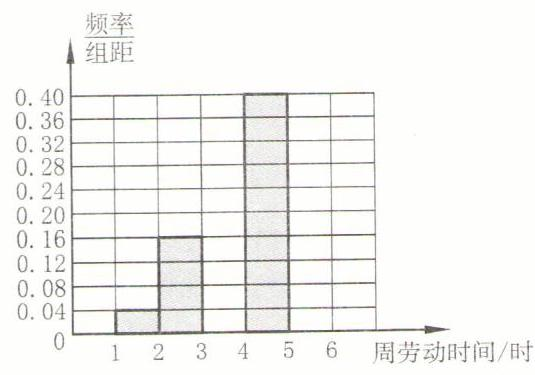
\includegraphics[width=0.4\textwidth]{bodyxb/src/bo_d20aucref24c73anc48g_246_980_1071_535_375_0.jpg}
\end{center}


(第 22 题)

(2)估计周劳动时间的平均数(同一组数据用该组区间的中点值为代表)；

(3)根据图表,估计周劳动时间的样本数据第 80 百分位数.

23. 某中学举行了一场诗词竞赛,组委会在赛后抽取了部分参赛选手的成绩(百分制)作为样本进行统计 (每组为左闭、右开的区间),作出了如图 1 的频率分布直方图和如图 2 的茎叶图 (中间三行污损, 看不清数据).

(第 23 题)

\begin{center}
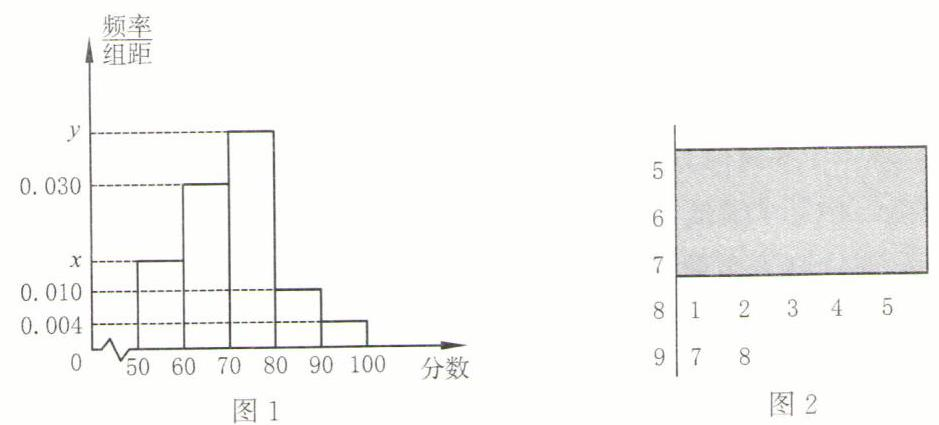
\includegraphics[width=0.8\textwidth]{bodyxb/src/bo_d20aucref24c73anc48g_246_407_1652_939_425_0.jpg}
\end{center}


(1)求样本容量 $n$ 和频率分布直方图中的 $x + y$ 的值；

(2)分数在 $\lbrack {80},{90})$ 的参赛选手中,男生有 3 人,现从该组抽取 3 人“座谈”. 请选择合适的表示方法写出样本空间, 并求至少有 1 名女生的概率.

24. 一家面包店以往每天制作 120 个三明治,为了解销售情况,店长统计了去年三明治的日销售量 (单位:个),并绘制频率分布直方图如图所示.

(1)求图中 $a$ 的值,并求该面包店去年(按 360 天算)三明治日销售量不少于 100 个的天数；

\begin{center}
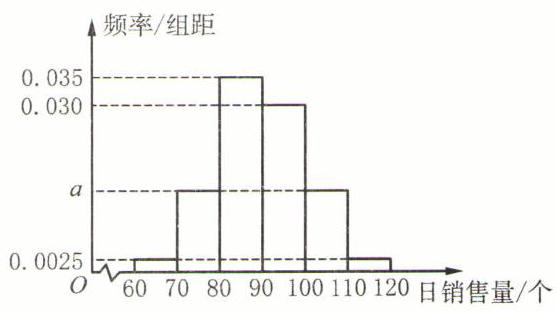
\includegraphics[width=0.4\textwidth]{bodyxb/src/bo_d20aucref24c73anc48g_247_891_370_556_314_0.jpg}
\end{center}


(第 24 题)

(2)估计该面包店去年三明治日销售量的平均数; (同一组中的数据以这组数据所在区间的中点值作代表)

(3)由于三明治的保质期只有一天,为了避免浪费,店长决定今年减少每天三明治的制作量, 但要求有 75\%的天数可以满足顾客的需求, 估计每天应该制作多少个三明治. (结果保留到整数)

25. 为贯彻“阳光体育”计划,促进学生身心素养的提高,某校倡导全校学生积极参与体育运动,并统计学生一周内运动时长,发现时长均在区间 $\left\lbrack  {2,{12}}\right\rbrack$ 内 (单位:时).

(1)将全校男生一周内运动时长分为 $\left\lbrack  {2,4}\right\rbrack  ,(4,6\rbrack$ , $(6,8\rbrack ,(8,{10}\rbrack ,({10},{12}\rbrack$ 五组,并绘制如图所示的频率分布直方图(同一组中的数据用该组区间的中点值代表). 估计该校男生一周运动时长的平均数 $\bar{x}$ 和中位数 $y$ ;

\begin{center}
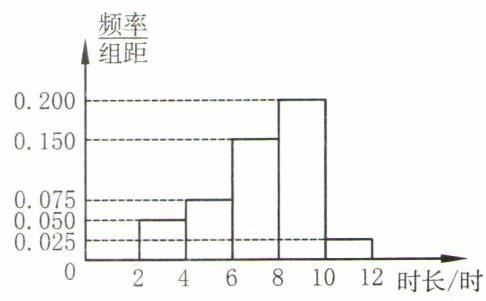
\includegraphics[width=0.4\textwidth]{bodyxb/src/bo_d20aucref24c73anc48g_247_961_991_486_301_0.jpg}
\end{center}


(第 25 题)

(2)已知高二(1)班男生 30 人,女生 20 人,根据数据统计分析, 发现该班男生一周内运动时长的平均数为 9 , 方差为 2 ; 女生一周内运动时长的平均数为 6.5, 方差为 4 . 求该班级全体学生一周内运动时长的方差 ${s}^{2}$ .

26. 某社区举办“闹元宵,猜灯谜”活动. 甲、乙、丙三个家庭同时参加此活动. 某一灯谜,已知甲家庭猜对的概率是 $\dfrac{3}{4}$ ,甲、丙两个家庭都猜错的概率是 $\dfrac{1}{12}$ ,乙、丙两个家庭都猜对的概率是 $\dfrac{1}{4}$ . 若各家庭是否猜对互不影响.

(1)求乙、丙两个家庭各自猜对此灯谜的概率；

(2)求甲、乙、丙三个家庭中不少于 2 个家庭猜对此灯谜的概率.

27. “数学好玩”是国际著名数学家陈省身赠送给少年数学爱好者们的一句话. 某校为了更好地培养学生的创新精神和实践能力,激发学生钻研数学的兴趣和热情,特举办数学节活动. 在活动中, 共有 20 道数学问题, 满分 100 分. 在所有的答卷成绩中随机抽取 100 份成绩作为样本,将样本分成六段: $\lbrack {40},{50}),\lbrack {50},{60}),\cdots ,\left\lbrack  {{90},{100}}\right\rbrack$ ,得到如图所示的频率分布直方图.

(1)求频率分布直方图中 $a$ 的值,并估计这次答卷所有成绩的中位数;

\begin{center}
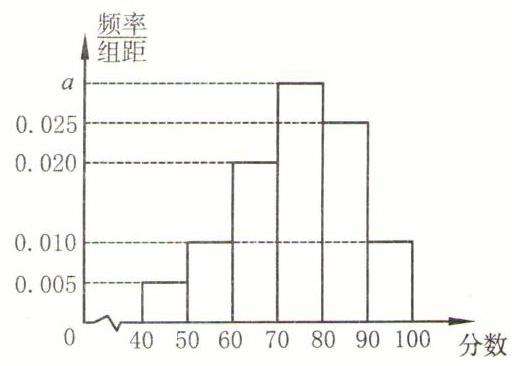
\includegraphics[width=0.4\textwidth]{bodyxb/src/bo_d20aucref24c73anc48g_248_983_139_512_366_0.jpg}
\end{center}


(第 27 题)

(2)活动中,甲、乙、丙三位同学独立答卷,已知甲同学答对了 12 道, 乙同学答对了 8 道, 丙同学答对了 $n$ 道,假设每道数学问题难度相当,被答对的可能性均相同.

①任选一道数学问题,求甲、乙两位同学恰有一人答对的概率.

② 任选一道数学问题,若甲、乙、丙三人中至少有一人答对的概率为 $\dfrac{22}{25}$ ,求 $n$ 的值.

\section*{(B)}

28. 为了迎接 2025 年第九届亚冬会的召开, 某班组织全班学生开展有关亚冬会知识的竞赛活动. 已知该班男生 35 人,女生 25 人,根据统计分析,男生组成绩和女生组成绩的方差分别为 ${s}_{1}^{2},{s}_{2}^{2}$ ,该班成绩的方差为 ${s}^{2}$ ,则下列结论一定正确的是 (   )

(A) ${s}^{2} = \dfrac{{s}_{1}^{2} + {s}_{2}^{2}}{2}$ . (B) ${s}^{2} \geq  \dfrac{{s}_{1}^{2} + {s}_{2}^{2}}{2}$ .

(C) ${s}^{2} = \dfrac{7{s}_{1}^{2} + 5{s}_{2}^{2}}{12}$ . (D) ${s}^{2} \geq  \dfrac{7{s}_{1}^{2} + 5{s}_{2}^{2}}{12}$ .

29. 在某次比赛中,某运动员五轮的成绩互不相等,记为 ${x}_{i}\left( {i = 1,2,3,4,5}\right)$ ,平均数为 $\bar{x}$ . 若随机删去其中一轮的成绩,得到一组新数据,记为 ${y}_{i}\left( {i = 1,2,3,4}\right)$ ,平均数为 $\bar{y}$ ,下面说法正确的是(   )

(A)新数据的极差不可能等于原数据的极差.

(B) 新数据的中位数可能等于原数据的中位数.

(C) 若 $\bar{x} = \bar{y}$ ,则新数据的方差可能小于原数据方差.

(D) 若 $\bar{x} = \bar{y}$ ,则新数据的第 40 百分位数一定大于原数据的第 40 百分位数.

30. 已知总体共划分为 3 层,通过分层随机抽样,各层抽取的样本容量分别为 ${n}_{1},{n}_{2},{n}_{3}$ ,样本平均数分别为 $\overline{{x}_{1}},\overline{{x}_{2}},\overline{{x}_{3}}$ ,样本方差分别为 ${s}_{1}^{2},{s}_{2}^{2},{s}_{3}^{2}$ . 若 ${n}_{1} : {n}_{2} : {n}_{3} = 1 : 2 : 3$ ,则(   )

(A) $\overline{{x}_{1}} : \overline{{x}_{2}} : \overline{{x}_{3}} = 1 : 2 : 3$ .

(B) ${s}_{1}^{2} : {s}_{2}^{2} : {s}_{3}^{2} = 1 : 4 : 9$ .

(C) 总体样本平均数 $\overline{x} = \overline{{x}_{1}} + 2\overline{{x}_{2}} + 3\overline{{x}_{3}}$ .

(D) 当 $\overline{{x}_{1}} = \overline{{x}_{2}} = \overline{{x}_{3}}$ 时,总体方差 ${s}^{2} = \dfrac{1}{6}{s}_{1}^{2} + \dfrac{1}{3}{s}_{2}^{2} + \dfrac{1}{2}{s}_{3}^{2}$ .

31. 水痘是一种传染性很强的病毒性疾病,容易在春天爆发,某市疾控中心为了调查某校高一年级学生注射水痘疫苗的人数,在高一年级随机抽取了 5 个班级,每个班级抽取的人数互不相同,若把每个班级抽取的人数作为样本数据,已知样本平均数为 5 ,样本方差为 4 ,则样本数据中的最大值为\blkda{}.

32. 为了解某校各班参加科技兴趣小组的人数, 从全校随机抽取 5 个班级, 设这 5 个班级参加科技兴趣小组的人数分别为 $x,y,z,m,n\left( {x < y < z < m < n,x,y,z,m,n \in  {\vv{n}}^{ * }}\right)$ . 已知这 5 个班级参加科技兴趣小组的人数的平均数为 9,方差为 4,则 z =\blkda{}.

33. 容量为 $n$ 的一组数据,它的第 $k$ 百分位数 ( $k$ 为 1 到 99 之间的整数) 各不相同,则 $n$ 的最小值为\blkda{}.

34. 校学生会希望调查有关本学期学生活动计划的意见, 你自愿担任调查员, 并打算在学校里抽取 10\% 的同学作为样本.

(1)你应怎样安排抽样,可保证样本的代表性？

(2)在抽样中,你可能会遇到哪些问题?

(3)这些问题可能会影响什么?

(4)你打算怎样解决这些问题?

35. 某机构对甲、乙两个工厂生产的一批零件随机抽取部分进行尺寸检测,统计所得数据分别画出了如图频率分布直方图:

\begin{center}
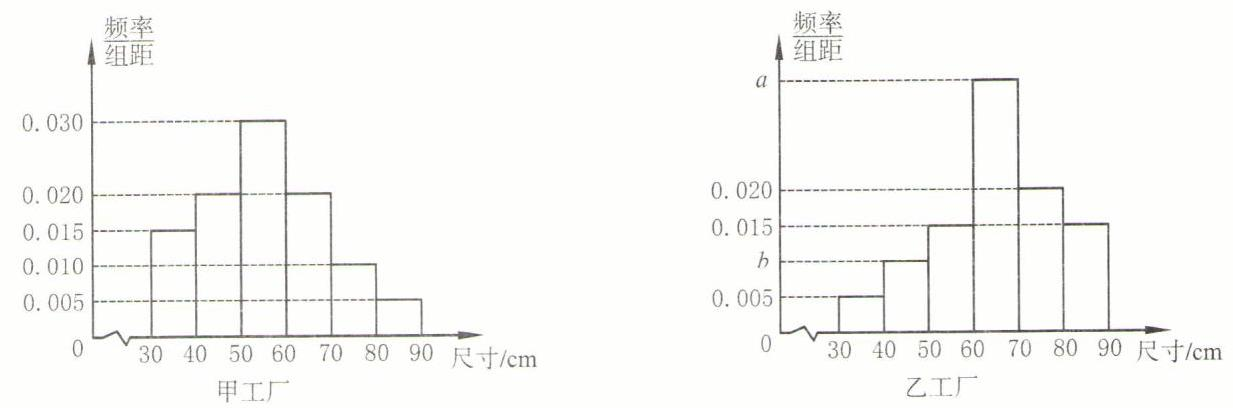
\includegraphics[width=1.0\textwidth]{bodyxb/src/bo_d20aucref24c73anc48g_249_175_871_1233_408_0.jpg}
\end{center}


(第 35 题)

根据乙工厂零件尺寸的频率分布直方图,估计事件“乙工厂生产的零件尺寸不低于 60cm” 的频率为 0.70 .

(1)估计甲工厂生产的这批零件尺寸的平均值；

(2)求乙工厂频率分布直方图中 $a,b$ 的值,及乙工厂被测零件尺寸的中位数(结果保留两位小数)；

(3)现采用分层抽样的方法,从甲工厂生产的零件中随机抽取尺寸在 $\lbrack {40},{50})$ 和 $\lbrack {70},{80})$ 内的零件 3 个, 从乙工厂生产的零件中随机抽取尺寸在 $\lbrack {40},{50})$ 和 $\lbrack {80},{90})$ 内的零件 5 个,再从抽得的 8 个零件中任取 2 个,求这 2 个零件的尺寸都在 $\lbrack {40},{50})$ 内的概率.

36. 已知某高速服务区餐厅的窗口有四类:① 自选快餐,平均每份取餐时长为 1 分钟；② 商务套餐,平均每份取餐时长为 0.5 分钟；③现炒现做,平均每份取餐时长为 5 分钟；④自动售货机,平均每份取餐时长为 1 分钟. 已知该高速服务区餐厅的取餐窗口(每台自动售货机按 1 个取餐窗口计算)一共有 18 个,就餐高峰期时有 400 名消费者在等待就餐. 为了提高消费者的用餐满意度, 该高速服务区工作人员选取了 100 名用餐的消费者进行问卷调查, 其中有 50 人选择了自选快餐, 30 人选择了商务套餐, 15 人选择了现炒现做, 5 人选择了自动售货机. (注:为了方便计算,若某消费者选择两类或多类就餐类别,则按该消费者的主要就餐类别归类,每名消费者只统计为其中一类).

(1)根据以上的调查统计,用样本估计总体,如果设置 10 个自选快餐窗口,就餐高峰期时, 假设大家在排队时自动选择较短的队伍等待(即各类取餐的窗口前队伍长度各自相等),试问选择自选快餐的消费者最长等待时长是多少分钟？

(2)根据以上的调查数据统计,用样本估计总体,从等待时长和公平的角度上考虑,要求每个队伍的最长等待时长大致相等,应如何设置各类取餐窗口数(结果采用四舍五入法保留整数)? 请说明理由.

37. 某学校组织“防电信诈骗知识”测试, 随机调查 400 名学生, 将他们的测试成绩(满分 100 分)的统计结果按 $\lbrack {50},{60}),\lbrack {60},{70}),\cdots ,\left\lbrack  {{90},{100}}\right\rbrack$ 依次分成第一组至第五组,得到如图所示的频率分布直方图.

(1)求图中 $x$ 的值；

\begin{center}
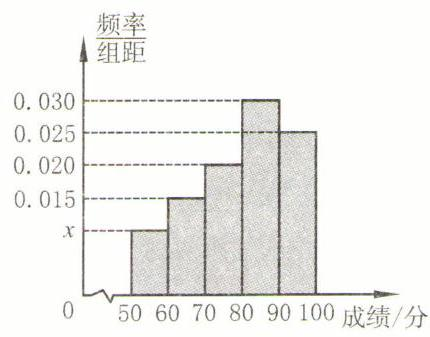
\includegraphics[width=0.3\textwidth]{bodyxb/src/bo_d20aucref24c73anc48g_250_1083_704_430_337_0.jpg}
\end{center}


(第 37 题)

(2)估计参与这次测试学生的成绩的平均数(同一组中的数据用该组区间的中点值为代表) 和第 60 百分位数;

(3)现从以上第三组、第四组和第五组参与测试的学生中用分层随机抽样的方法选取 15 人,担任学校“防电信诈骗知识”的宣传员. 若这 15 名学校宣传员中来自第三组学生的测试成绩的平均数和方差分别为 75 和 5 , 来自第四组学生的测试成绩的平均数和方差分别为 85 和 10 , 来自第五组学生的测试成绩的平均数和方差分别为 93 和 5.2 , 据此估计第三组、第四组和第五组所有参与测试学生的成绩的方差.

38. 假设 $\mathrm{L}$ 市 4 月的天气情况有晴天、雨天、阴天三种,第二天的天气情况只取决于前一天的天气情况,与再之前的天气情况无关. 若前一天为晴天,则第二天下雨的概率为 $\dfrac{1}{4}$ ,阴天的概率为 $\dfrac{1}{4}$ ; 若前一天为下雨,则第二天晴天的概率为 $\dfrac{1}{4}$ ,阴天的概率为 $\dfrac{3}{8}$ ; 若前一天为阴天, 则第二天晴天的概率为 $\dfrac{1}{4}$ ,下雨的概率为 $\dfrac{1}{3}$ ; 已知 $\mathrm{L}$ 市 4 月第 1 天的天气情况为下雨.

(1)求 L 市 4 月第 3 天的天气情况为晴天的概率；

(2)记 ${a}_{n}$ 为 $\mathrm{L}$ 市 4 月第 $n\left( {n \in  \vv{n},1 \leq  n \leq  {30}}\right)$ 天的天气情况为晴天的概率,

①求 ${a}_{n}$ 的通项公式;

②L市某花卉种植基地计划在 4 月根据天气情况种植向日葵, 为了更好地促进向日葵种子的发芽和生长,要求提前 3 天对种子进行特殊处理, 并尽可能地选择在晴天种植. 如果你是该花卉种植基地的气象顾问, 根据上述计算结果, 请你对该基地的种植计划提出建议.

39. 甲、乙、丙三位同学进行乒乓球比赛,约定赛制如下:每场比赛胜者积 2 分,负者积 0 分；比赛前根据相关规则决定首先比赛的两人,另一人轮空；每场比赛的胜者与轮空者进行下一场比赛,负者下一场轮空；积分首先累计到 4 分者获得比赛胜利,比赛结束. 已知甲与乙比赛时,甲获胜的概率为 ${p}_{1}$ ,甲与丙比赛时,甲获胜的概率为 ${p}_{2}$ ,乙与丙比赛时,乙获胜的概率为 ${p}_{3}$ . 若 ${p}_{1} + {p}_{3} > 1$ ,假设乙获得了指定首次比赛选手的权利,为获得比赛的胜利,试分析乙的最优指定策略.

40. 给定两组数据 $A = \left( {{x}_{1},{x}_{2},\cdots ,{x}_{n}}\right)$ 与 $B = \left( {{y}_{1},{y}_{2},\cdots ,{y}_{n}}\right)$ ,称 $X\left( {A,B}\right)  = \mathop{\sum }\limits_{{i = 1}}^{n}\left| {{x}_{i} - {y}_{i}}\right|$ 为这两组数据之间的“差异量”. 鉴宝类的节目是当下非常流行的综艺节目. 现有 $n$ 个古董,它们的价值各不相同,最值钱的古董记为 1 号,第二值钱的古董记为 2 号,以此类推,则古董价值的真实排序为 $I = \left( {1,2,\cdots ,n}\right)$ . 现在某专家在不知道古董真实排序的前提下,根据自已的经验对这 $n$ 个古董的价值从高到低依次进行重新排序为 ${x}_{1},{x}_{2},\cdots ,{x}_{n}$ ,其中 ${x}_{i}$ 为该专家给真实价值排第 $i$ 位古董的位次编号,记 $A = \left( {{x}_{1},{x}_{2},\cdots ,{x}_{n}}\right)$ ,那么 $A$ 与 $I$ 的差异量 $X\left( {A,I}\right)  = \mathop{\sum }\limits_{{i = 1}}^{n}\left| {{x}_{i} - i}\right|$ 可以有效反映一个专家的水平,该差异量 $X\left( {A,I}\right)$ 越小说明专家的鉴宝能力越强.

(1)当 $n = 3$ 时,求 $X\left( {A,I}\right)$ 的所有可能取值；

(2)当 $n = 5$ 时,求 $X\left( {A,I}\right)  = 4$ 的概率；

(3)现在有两个专家甲、乙同时进行鉴宝,已知专家甲的鉴定结果与真实价值 $I$ 的差异量为 $a$ ,专家甲与专家乙的鉴定结果的差异量为 4 ,那么专家乙的鉴定结果与真实价值 $I$ 的差异量是否可能为 $a + 6$ ? 请说明理由.

\section*{二、条件概率与相关公式}

\section*{【典型题型和解题技巧】}

例 1 从含甲、乙在内的 5 名全国第七次人口普查员中随机选取 3 人到某小区进行人口普查,求在甲被选中的条件下,乙也被选中的概率.

解 方法一:记事件 $A$ 为 “甲被选中”,事件 $B$ 为 “乙被选中”,则由题意可得

$P\left( A\right)  = \dfrac{{\mathrm{C}}_{4}^{2}}{{\mathrm{C}}_{5}^{3}} = \dfrac{6}{10} = \dfrac{3}{5},P\left( {A \cap  B}\right)  = \dfrac{{\mathrm{C}}_{3}^{1}}{{\mathrm{C}}_{5}^{3}} = \dfrac{3}{10},$

所以 $P\left( {B \mid  A}\right)  = \dfrac{P\left( {A \cap  B}\right) }{P\left( A\right) } = \dfrac{3}{10} \times  \dfrac{5}{3} = \dfrac{1}{2}$ .

方法二:记事件 $A$ 为“甲被选中”,事件 $B$ 为“乙被选中”,

将事件 $A$ 当作新的样本空间,则其中有 ${\mathrm{C}}_{4}^{2} = 6$ 个样本点,其中甲、乙被同时选中的样本点有 ${\mathrm{C}}_{3}^{1} = 3$ 个,所以 $P\left( {B \mid  A}\right)  = \dfrac{3}{6} = \dfrac{1}{2}$ .

注意 1. 求条件概率的常用方法

(1)利用定义,分别求 $P\left( A\right)$ 和 $P\left( {A \cap  B}\right)$ ,得 $P\left( {B \mid  A}\right)  = \dfrac{P\left( {A \cap  B}\right) }{P\left( A\right) }$ .

(2)光求事件 $A$ 包含的样本点个数 $\left| A\right|$ ,再在事件 $A$ 发生的条件下求事件 $B$ 包含的样本点个数,即 $\left| {A \cap  B}\right|$ ,得 $P\left( {B \mid  A}\right)  = \dfrac{\left| A \cap  B\right| }{\left| A\right| }$ .

2. 条件概率的性质: ① $P\left( {\Omega  \mid  A}\right)  = 1$ ;

②若 $B,C$ 是两个互斥事件,则 $P\left( {B \cup  C \mid  A}\right)  = P\left( {B \mid  A}\right)  + P\left( {C \mid  A}\right)$ ；

③ 设 $B$ 和 $\bar{B}$ 互为对立事件,则 $P\left( {\bar{B} \mid  A}\right)  = 1 - P\left( {B \mid  A}\right)$ .

3. 由条件概率公式可得 $P\left( {A \cap  B}\right)  = P\left( A\right)  \cdot  P\left( {B \mid  A}\right)$ ,该公式称为概率的乘法公式,具体应用请看下面的例子.

例 2 已知 1 号箱中有 2 个白球和 4 个红球, 2 号箱中有 5 个白球和 3 个红球. 现随机从 1 号箱中取出一球放入 2 号箱, 然后从 2 号箱中随机取出一球, 求两次都取到红球的概率.

解 设 “从 1 号箱取到红球” 为事件 $A$ ,“从 2 号箱取到红球” 为事件 $B$ .

由题意, $P\left( A\right)  = \dfrac{4}{6} = \dfrac{2}{3},P\left( {B \mid  A}\right)  = \dfrac{3 + 1}{8 + 1} = \dfrac{4}{9}$ ,

所以 $P\left( {A \cap  B}\right)  = P\left( A\right)  \cdot  P\left( {B \mid  A}\right)  = \dfrac{2}{3} \times  \dfrac{4}{9} = \dfrac{8}{27}$ ,即两次都取到红球的概率为 $\dfrac{8}{27}$ .

例 3 某卡车为乡村小学运送书籍, 共装有 10 个纸箱, 其中 5 箱英语书、 2 箱数学书、 3 箱语文书. 到目的地时发现丢失一箱,但不知丢失哪一箱,现从剩下的 9 箱中任意打开两箱,求结果都是英语书的概率.

解 设事件 $A$ 表示丢失一箱后任取两箱是英语书,事件 ${B}_{k}$ 表示丢失一箱为 $k$ (其中 $k = 1$ , 2,3,分别表示英语书、数学书、语文书),

可得 $P\left( A\right)  = P\left( {B}_{1}\right) P\left( {A \mid  {B}_{1}}\right)  + P\left( {B}_{2}\right) P\left( {A \mid  {B}_{2}}\right)  + P\left( {B}_{3}\right) P\left( {A \mid  {B}_{3}}\right)$

$= \dfrac{1}{2} \times  \dfrac{{\mathrm{C}}_{4}^{2}}{{\mathrm{C}}_{9}^{2}} + \dfrac{1}{5} \times  \dfrac{{\mathrm{C}}_{5}^{2}}{{\mathrm{C}}_{9}^{2}} + \dfrac{3}{10} \times  \dfrac{{\mathrm{C}}_{5}^{2}}{{\mathrm{C}}_{9}^{2}} = \dfrac{2}{9}.$

注意 设样本空间 $\Omega$ 可分成 $n$ 个两两互斥的事件 ${\Omega }_{1},{\Omega }_{2},\cdots ,{\Omega }_{n}$ ,且 $P\left( {\Omega }_{i}\right)  > 0,i = 1,2$ , $\cdots ,n$ ,则对任意的事件 $A \subseteq  \Omega$ ,有

\[
P\left( A\right)  = \mathop{\sum }\limits_{{k = 1}}^{n}P\left( {A \mid  {\Omega }_{k}}\right)  \cdot  P\left( {\Omega }_{k}\right) ,
\]

上述公式称为全概率公式. 全概率公式是概率的可加性与乘法公式的组合.

例 4 三个罐子分别编号为 1,2,3,其中 1 号罐中装有 2 个红球和 1 个黑球,2 号罐中装有 3 个红球和 1 个黑球,3 号罐中装有 2 个红球和 2 个黑球. 若某人从中随机取一罐,再从中任意取出一球, 求取得红球的概率.

解 记 ${B}_{i} = \{$ 球取自 $i$ 号罐 $\} \left( {i = 1,2,3}\right) ,A = \{$ 取得红球 $\}$ ,显然 $A$ 的发生总是伴随着 ${B}_{1}$ , ${B}_{2},{B}_{3}$ 之一同时发生,即 $A = \left( {A \cap  {B}_{1}}\right)  \cup  \left( {A \cap  {B}_{2}}\right)  \cup  \left( {A \cap  {B}_{3}}\right)$ ,且 $A \cap  {B}_{1},A \cap  {B}_{2},A \cap  {B}_{3}$ 两两互斥, $P\left( {A \mid  {B}_{1}}\right)  = \dfrac{2}{3},P\left( {A \mid  {B}_{2}}\right)  = \dfrac{3}{4},P\left( {A \mid  {B}_{3}}\right)  = \dfrac{1}{2}$ ,

所以 $P\left( A\right)  = P\left( {A \cap  {B}_{1}}\right)  + P\left( {A \cap  {B}_{2}}\right)  + P\left( {A \cap  {B}_{3}}\right)$

$= \mathop{\sum }\limits_{{i = 1}}^{3}P\left( {B}_{i}\right) P\left( {A \mid  {B}_{i}}\right)  = \dfrac{1}{3} \times  \dfrac{2}{3} + \dfrac{1}{3} \times  \dfrac{3}{4} + \dfrac{1}{3} \times  \dfrac{1}{2} = \dfrac{23}{36}.$

注意 全概率公式的意义在于,当直接计算事件 $\Lambda$ 发生的概率 $P\left( \Lambda \right)$ 较为困难时,可以先找到样本空间 $\Omega$ 的一个划分 ${\Omega }_{1},{\Omega }_{2},\cdots ,{\Omega }_{n}$ : 满足 $\Omega  = {\Omega }_{1} \cup  {\Omega }_{2} \cup  \cdots  \cup  {\Omega }_{n}$ ,且 ${\Omega }_{1},{\Omega }_{2},\cdots ,{\Omega }_{n}$ 两两互斥. 将 ${\Omega }_{1},{\Omega }_{2},\cdots ,{\Omega }_{n}$ 看成是导致事件 $A$ 发生的一组原因,这样事件 $A$ 就被分解成了 $n$ 个部分,可以分别计算 $P\left( {A \mid  {\Omega }_{1}}\right) ,P\left( {A \mid  {\Omega }_{2}}\right) ,\cdots ,P\left( {A \mid  {\Omega }_{n}}\right)$ ,再利用全概率公式求解.

* 例 5 假设某种疾病在所有人群中的感染率是 0.1\%,医院现有的技术对于该疾病检测准确率为 ${99}\%$ ,即在已知患病情况下,有 ${99}\%$ 的可能性检测结果为阳性,正常人有 ${99}\%$ 的可能性检测结果为阴性. 现从人群中随机抽一人去检测,求在医院给出的检测结果为阳性的条件下此人得病的概率.

解 记“一人得病”为事件 $A$ ,“检测结果为阳性”为事件 $B$ ,

则 $P\left( A\right)  = {0.1}\% ,P\left( {B \mid  A}\right)  = {99}\% ,P\left( {B \mid  A}\right)  \cdot  P\left( A\right)  + P\left( {B \mid  \bar{A}}\right)  \cdot  P\left( \bar{A}\right)  = {0.01098}$ ,

所以 $P\left( {A \mid  B}\right)  = \dfrac{P\left( {B \mid  A}\right)  \cdot  P\left( A\right) }{P\left( {B \mid  A}\right)  \cdot  P\left( A\right)  + P\left( {B \mid  \bar{A}}\right)  \cdot  P\left( \bar{A}\right) } = \dfrac{{99}\%  \times  {0.1}\% }{0.010} = \dfrac{11}{122} \approx  9\%$ ,

所以在医院给出的检测结果为阳性的条件下此人得病的概率约为 9\%.

注意 1. 在事件 $A$ 发生的条件下,事件 ${\Omega }_{i}$ 发生的概率为

\[
P\left( {{\Omega }_{i} \mid  A}\right)  = \dfrac{P\left( {A \mid  {\Omega }_{i}}\right)  \cdot  P\left( {\Omega }_{i}\right) }{\mathop{\sum }\limits_{{k = 1}}^{n}P\left( {A \mid  {\Omega }_{k}}\right)  \cdot  P\left( {\Omega }_{k}\right) }
\]

上述公式称为贝叶斯公式.

2. 在上述例子中,事件 $A$ 是检测结果为阳性的原因, $P\left( A\right)$ 与 $P\left( \bar{A}\right)$ 称为先验概率,它们反映了各种原因发生的可能性大小,现在试验的结果是事件 $B$ 发生了,这个信息将有助于研究事件发生的原因, $P\left( {A \mid  B}\right)$ 与 $P\left( {\bar{A} \mid  B}\right)$ 称为后验概率,它们反映了试验之后对各种原因发生的可能性大小的新的认识. 贝叶斯公式告诉我们,事件的概率可以根据出现的新信息进行修正. 这是一种统计学的哲学观点, 也是人工智能蓬勃发展的基础之一.

\section*{【训练题】}

\section*{(A)}

41. 甲、乙两个小组各 10 名学生的数学测试成绩如下(单位:分).

甲组:76,90,84,86,81,87,86,82,85,83

乙组:82,84,85,89,79,80,91,89,79,74

现从这 20 名学生中随机抽取一人,将 “抽出的学生为甲组学生” 记为事件 $A$ , “抽出的学生的数学测试成绩不低于 85 分”记为事件 $B$ ,则 $P\left( {A \mid  B}\right)$ 的值是 (   )

(A) $\dfrac{5}{9}$ . (B) $\dfrac{4}{9}$ . (C) $\dfrac{2}{9}$ . (D) $\dfrac{1}{9}$ .

42. 已知 $\bar{A},\bar{B}$ 分别为随机事件 $A,B$ 的对立事件, $P\left( A\right)  > 0,P\left( B\right)  > 0$ ,则下列等式错误的是(   )

(A) $P\left( {B \mid  A}\right)  + P\left( {\bar{B} \mid  A}\right)  = P\left( A\right)$ . (B) $P\left( {B \mid  A}\right)  + P\left( {\bar{B} \mid  A}\right)  = 1$ .

(C) 若 $A,B$ 独立,则 $P\left( {A \mid  B}\right)  = P\left( A\right)$ . (D) 若 $A,B$ 互斥,则 $P\left( {A \mid  B}\right)  = P\left( {B \mid  A}\right)$ .

43. 掷两枚均匀的大小不同的骰子,记“两枚骰子的点数和为 10 ”为事件 $A$ ,“小骰子出现的点数大于大骰子出现的点数”为事件 $B$ ,则 $P\left( {B \mid  A}\right)$ 为(   )

(A) $\dfrac{1}{2}$ . (B) $\dfrac{1}{6}$ . (C) $\dfrac{1}{15}$ . (D) $\dfrac{1}{3}$ .

44. 从编号为 1-20 的 20 张卡片中依次不放回地抽出两张,记事件 $A$ 为 “第一次抽到数为 6 的倍数”, $B$ 为“第二次抽到的数小于第一次抽到的数”,则 $P\left( {B \mid  A}\right)  =$ (   )

(A) $\dfrac{8}{19}$ . (B) $\dfrac{11}{19}$ . (C) $\dfrac{8}{11}$ . (D) $\dfrac{7}{19}$ .

45. 设某种动物由出生算起活到 20 岁的概率为 0.8 , 活到 25 岁的概率为 0.4 , 现有一个 20 岁的这种动物,它能活到 25 岁的概率是\blkda{}.

46. 从1,2,3,4,5,6,7,8,9中不放回地依次取 2 个数,事件 $A$ 为 “第一次取到的是奇数”,事件 $B$ 为“第二次取到的是 3 的整数倍”,则 $P\left( {B \mid  A}\right)  =$ \blkda{}.

47. 长时间玩手机可能影响视力,据调查,某校学生大约 30\% 的人近视,而该校大约有 40\% 的学生每天玩手机超过 $2\mathrm{h}$ ,这些人的近视率约为 ${60}\%$ ,现从该校近视的学生中任意调查一名学生,则他每天玩手机超过 $2\mathrm{h}$ 的概率为\blkda{}.

48. 某企业将生产出的芯片依次进行智能检测和人工检测两道检测工序, 经智能检测为次品的芯片会被自动淘汰,合格的芯片进入流水线并由工人进行人工检验. 已知某批芯片智能自动检测显示合格率为 ${90}\%$ ,最终的检测结果的次品率为 $\dfrac{3}{10}$ ,则在智能自动检测结束并淘汰了次品的条件下,人工检测一枚芯片恰好为合格品的概率为\blkda{}.

49. 已知随机事件 $A,B,P\left( A\right)  = \dfrac{1}{3},P\left( B\right)  = \dfrac{1}{4},P\left( {A \mid  B}\right)  = \dfrac{3}{4}$ ,则 $P\left( {\bar{B} \mid  A}\right)  =$ \blkda{}.

50. 研究人员开展甲、乙两种药物的临床抗药性研究实验,事件 $A$ 为 “对药物甲产生抗药性”, 事件 $B$ 为 “对药物乙产生抗药性”,事件 $C$ 为 “对甲、乙两种药物均不产生抗药性”. 若 $P\left( A\right)  = \dfrac{4}{15},P\left( B\right)  = \dfrac{2}{15},P\left( C\right)  = \dfrac{7}{10}$ ,则 $P\left( {B \mid  A}\right)  =$ \blkda{}.

51. 某商店收进甲厂生产的产品 30 箱, 乙厂生产的同种产品 20 箱, 甲厂每箱装 100 个, 废品率为 0.06 ,乙厂每箱装 120 个,废品率为 0.05 ,求:

(1)任取一箱,从中任取一个产品为废品的概率；

(2)若将所有产品开箱混放,求任取一个产品为废品的概率.

52. 某学校安排甲、乙、丙三个班同时到学校礼堂参加联欢晚会, 已知甲班艺术特长生占比 $8\%$ ,乙班艺术特长生占比 $6\%$ ,丙班艺术特长生占比 $5\%$ . 学生自由选择座位,先到者先选. 甲、乙、丙三个班人数分别占总人数的 $\dfrac{1}{4},\dfrac{1}{3},\dfrac{5}{12}$ . 若主持人随机从场下学生中选一人参与互动.

(1)求选到的学生是艺术特长生的概率；

(2)如果选到的学生是艺术特长生,判断其来自哪个班的可能性最大.

53. 小张从家到公司上班总共有三条路可以走 (如图), 但是每条路每天拥堵的可能性不太一样, 由于远近不同, 选择每条路的概率分别为 $P\left( {L}_{1}\right)  = {0.5},P\left( {L}_{2}\right)  = {0.3},P\left( {L}_{3}\right)  = {0.2}$ , 每天上述三条路不拥堵的概率分别为 $P\left( {C}_{1}\right)  = {0.2},P\left( {C}_{2}\right)$  $= {0.4},P\left( {C}_{3}\right)  = {0.7}$ .

\begin{center}
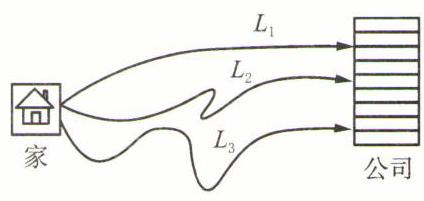
\includegraphics[width=0.3\textwidth]{bodyxb/src/bo_d20aucref24c73anc48g_255_1030_132_424_201_0.jpg}
\end{center}


(第 53 题)

(1)小张从家到公司未遇上拥堵的概率是多少？

(2)已知小张从家到公司未遇上拥堵,他选择道路 ${L}_{1}$ 的概率是多少？

\section*{(B)}

54. 已知 $P\left( A\right)  = {0.4},P\left( {B \mid  A}\right)  = {0.2},P\left( {B \mid  \bar{A}}\right)  = {0.3}$ ,则 $P\left( \bar{B}\right)  =$ \blkda{}.

55. 已知 $P\left( A\right)  = \dfrac{1}{2},P\left( {B \mid  A}\right)  = \dfrac{1}{4},P\left( {\overset{―}{B} \mid  \overset{―}{A}}\right)  = \dfrac{2}{3}$ ,则 $P\left( B\right)  =$ \blkda{}.

56. 质数 (prime number) 又称素数,一个大于 1 的自然数,除了 1 和它本身外,不能被其他自然数整除, 则这个数为质数, 数学上把相差为 2 的两个素数叫作 “孪生素数”. 如: 3 和 5, 5 和 7 ……,在 1900 年的国际数学大会上,著名数学家希尔伯特提出了 23 个问题,其中第 8 个就是大名鼎鼎的孪生素数猜想:即存在无穷多对孪生素数. 我国著名数学家张益唐 2013 年在《数学年刊》上发表论文《素数间的有界距离》,破解了困扰数学界长达一个半世纪的难题,证明了孪生素数猜想的弱化形式. 那么,如果我们在不超过 30 的自然数中,随机选取两个不同的数,记事件 $A =$ “这两个数都是素数”,事件 $B =$ “这两个数不是孪生素数”,那么 $P\left( {B \mid  A}\right)  =$ \blkda{}.

57. 据调查,某地市民大约有 0.03\% 的人患某种疾病,该地大约有 0.1\% 的市民有超过 20 年的时间有某种不良饮食习惯,这些人患这种疾病的人约为 10\% . 现从饮食不良习惯不超过 20 年的市民中随机抽取 1 名市民,则他患此疾病的概率约为\blkda{}\%(精确到 0.01\%).

58. 在某次美术专业测试中,若甲、乙、丙三人获得优秀等级的概率分别是 0.6,0.7 和 0.5 , 且三人的测试结果相互独立,则测试结束后,在甲、乙、丙三人中恰有两人没达优秀等级的前提条件下,乙没有达优秀等级的概率为\blkda{}.

59. 假设你正在参加一个电视节目,舞台上有三扇门,其中一扇门的后面是汽车,另外两扇门的后面是山羊,如果你选中了后面有汽车的那扇门,就可以得到这辆汽车. 现在你随机选择了一扇门, 走到门前, 但还未打开. 这时, 主持人打开了另外两扇门中的一扇, 让你看到了那扇门的后面是一只山羊 (主持人清楚每扇门后面都是什么). 现在,主持人给你一次重新选择的机会. 假设你选择换另一扇还未打开的门,那么得到汽车的概率是\blkda{}.

60. 杭州第 19 届亚运会于 2023 年 9 月 23 日至 10 月 8 日举办, 组委会将甲、乙、丙、丁 4 名志愿者随机派往黄龙体育中心、杭州奥体中心、浙江大学紫金港校区三座体育馆工作,每座体育馆至少派 1 名志愿者,事件 $A$ 表示 “志愿者甲派往黄龙体育中心”,事件 $B$ 表示 “志愿者乙派往黄龙体育中心”,事件 $C$ 表示“志愿者乙派往杭州奥体中心”,则(   )

(A) 事件 $A$ 与 $B$ 相互独立. (B) 事件 $A$ 与 $C$ 为互斥事件.

(C) $P\left( {C \mid  A}\right)  = \dfrac{1}{3}$ . (D) $P\left( {B \mid  A}\right)  = \dfrac{1}{6}$ .

61. 已知事件 $A,B$ 满足 $0 < P\left( A\right)  < 1,0 < P\left( B\right)  < 1$ ,则不能说明事件 $A,B$ 相互独立的是(   )

(A) $P\left( {A \mid  B}\right)  = P\left( {\bar{A} \mid  B}\right)$ . (B) $P\left( {A \mid  B}\right)  = P\left( A\right)$ .

(C) $P\left( {B \mid  A}\right)  = P\left( B\right)$ . (D) $P\left( {B \mid  A}\right)  = P\left( {B \mid  \bar{A}}\right)$ .

62. 已知 $A,B$ 为两个随机事件, $P\left( A\right) ,P\left( B\right)  > 0$ ,则 “ $A,B$ 相互独立” 是 “ $P\left( {\bar{A} \mid  B}\right)  = P(\bar{A}$  $\bar{B})$ ”的(   )

(A) 充分非必要条件. (B) 必要非充分条件.

(C) 充要条件. (D) 既非充分又非必要条件.

63. 甲罐中有 5 个红球, 2 个白球和 3 个黑球, 乙罐中有 4 个红球, 3 个白球和 3 个黑球(球除颜色外,大小、质地均相同). 先从甲罐中随机取出一球放入乙罐,分别以事件 ${A}_{1},{A}_{2}$ 和 ${A}_{3}$ 表示由甲罐中取出的球分别是红球、白球和黑球; 再从乙罐中随机取出一球,以事件 $B$ 表示由乙罐中取出的球分是红球. 下列结论正确的个数是(   )

①事件 ${A}_{1}$ 与 ${A}_{2}$ 相互独立; ② $P\left( {B \mid  {A}_{2}}\right)  = \dfrac{4}{11}$ ; ③ $P\left( B\right)  = \dfrac{9}{22}$ ; ④ $P\left( {{A}_{1} \mid  B}\right)  = \dfrac{4}{9}$ .

(A) 4. (B) 3. (C) 2 . (D) 1 .

64. 根据某机构对失踪飞机的调查得知:失踪的飞机中有 70\% 的飞机后来被找到,在被找到的飞机中,有 60\% 安装有紧急定位传送器,而未被找到的失踪飞机中,有 90\% 未安装紧急定位传送器. 紧急定位传送器是在飞机失事坠毁时发送信号,让搜救人员可以定位的装置. 现有一架安装有紧急定位传送器的飞机失踪,则它被找到的概率为(   )

(A) $\dfrac{14}{23}$ . (B) $\dfrac{28}{55}$ . (C) $\dfrac{14}{15}$ . (D) $\dfrac{27}{55}$ .

65. 随着城市经济的发展,早高峰问题越发严重,上班族需要选择合理的出行方式. 某公司员工小明的上班出行方式有三种,某天早上他选择自驾、坐公交车、骑共享单车的概率分别为 $\dfrac{1}{3},\dfrac{1}{3},\dfrac{1}{3}$ ,而他自驾、坐公交车、骑共享单车迟到的概率分别为 $\dfrac{1}{4},\dfrac{1}{5},\dfrac{1}{6}$ ,结果这一天他迟到了, 在此条件下, 他自驾去上班的概率是 (   )

(A) $\dfrac{12}{37}$ . (B) $\dfrac{15}{37}$ . (C) $\dfrac{3}{5}$ . (D) $\dfrac{4}{7}$ .

66. AI 换脸是一项深度伪造技术, 某视频网站利用该技术掺入了一些 “AI”视频, “AI”视频占比为 0.1\%. 某团队决定用 AI 对抗 AI, 研究了深度鉴伪技术来甄别视频的真假. 该鉴伪技术的准确率是 0.98 ,即在该视频是伪造的情况下,它有 98\% 的可能鉴定为 “AI”; 它的误报率是 0.04 ,即在该视频是真实的情况下,它有 $4\%$ 的可能鉴定为 “AI”. 已知某个视频被鉴定为“AI”,则该视频是“AI”合成的可能性为(   )

(A) ${0.1}\%$ . (B) ${0.4}\%$ . (C) ${2.4}\%$ . (D) $4\%$ .

67. 根据以往的临床记录,某种诊断癌症的试验有如下的效果,若以 $A$ 表示事件“试验反应为

阳性”,以 $C$ 表示事件“被诊断者患有癌症”,则有 $P\left( {A \mid  C}\right)  = {0.95},P\left( {\bar{A} \mid  \bar{C}}\right)  = {0.95}$ . 现在对自然人群进行普查,设被试验的人患有癌症的概率为 0.005 ,即 $P\left( C\right)  = {0.005}$ ,则 $P\left( {C \mid  A}\right)  \approx$ (   )

(A) 0.087 . (B) 0.950 . (C) 0.050. (D) 0.475 .

68. 某运动队为评估短跑运动员在接力赛中的作用,对运动员进行数据分析. 运动员甲在接力赛中跑第一棒、第二棒、第三棒、第四棒四个位置,统计以往多场比赛,其出场率与出场时比赛获胜率如下表所示.

\begin{center}
\adjustbox{width=\textwidth}{
\begin{tabular}{|c|c|c|c|c|}
\hline
比赛位置 & 第一棒 & 第二棒 & 第三棒 & 第四棒 \\
\cline{1-5}
出场率 & 0.3 & 0.2 & 0.2 & 0.3 \\
\cline{1-5}
比赛胜率 & 0.6 & 0.8 & 0.7 & 0.7 \\
\cline{1-5}
\hline
\end{tabular}
}
\end{center}

(1)当甲出场比赛时,求该运动队获胜的概率；

(2)当甲出场比赛时,在该运动队获胜的条件下,求甲跑第一棒的概率；

(3)如果你是教练员,将如何安排运动员甲比赛时的位置？并说明理由.

69. 在数字通信中, 信号是由数字 0 和 1 组成的序列, 且传输相互独立. 由于随机因素的干扰, 发送的信号 0 或 1 有可能被错误地接收为 1 或 0 . 已知发送 0 时,收到 1 的概率为 $\alpha (0 < \alpha$  $< 1)$ ,收到 0 的概率为 $1 - \alpha$ ; 发送 1 时,收到 0 的概率为 $\beta \left( {0 < \beta  < 1}\right)$ ,收到 1 的概率为 1- $\beta$ . 假设发送信号 0 和 1 是等可能的.

(1)已知接收的信号为 1,且 $\alpha  = {0.1},\beta  = {0.05}$ ,求发送的信号是 0 的概率；

(2)现有两种传输方案:单次传输和三次传输. 单次传输是指每个信号只发送 1 次；三次传输是指每个信号重复发送 3 次. 收到的信号需要译码, 译码规则如下: 单次传输时, 收到的信号即为译码；三次传输时,收到的信号中出现次数多的即为译码(例如,若依次收到 1,0,1 . 则译码为 1 ). 已知发送 1,若采用三次传输方案译码为 1 的概率大于采用单次传输方案译码为 1 的概率,求 $\beta$ 的取值范围.

70. 一医疗团队为研究某地的一种地方性疾病与当地居民的卫生习惯(卫生习惯分为良好和不够良好两类)的关系,在已患该疾病的病例中随机调查了 100 例(称为病例组),同时在未患该疾病的人群中随机调查了 100 人(称为对照组),得到如下数据:

\begin{center}
\adjustbox{width=\textwidth}{
\begin{tabular}{|c|c|c|}
\hline
\phantom{X} & 不够良好 & 良好 \\
\cline{1-3}
病例组 & 40 & 60 \\
\cline{1-3}
对照组 & 10 & 90 \\
\cline{1-3}
\hline
\end{tabular}
}
\end{center}

从该地的人群中任选一人, $A$ 表示事件 “选到的人卫生习惯不够良好”, $B$ 表示事件 “选到的人患有该疾病”. $\dfrac{P\left( {B \mid  A}\right) }{P\left( {\bar{B} \mid  A}\right) }$ 与 $\dfrac{P\left( {\bar{B} \mid  \bar{A}}\right) }{P\left( {\bar{B} \mid  \bar{A}}\right) }$ 的比值是卫生习惯不够良好对患该疾病风险程度的一项度量指标,记该指标为 $R$ .

(1) 证明: $R = \dfrac{P\left( {A \mid  B}\right) }{P\left( {\bar{A} \mid  B}\right) } \cdot  \dfrac{P\left( {\bar{A} \mid  \bar{B}}\right) }{P\left( {A \mid  \bar{B}}\right) }$ ;

(2)利用该调查数据,给出 $P\left( {A \mid  B}\right) ,P\left( {A \mid  \bar{B}}\right)$ 的估计值,并利用 (1) 的结果给出 $R$ 的估计值.

\section*{三、随机变量的分布与特征、常用分布}

\section*{【典型题型和解题技巧】}

例 1 设一汽车在行进途中要经过 4 个路口,在每个路口遇到绿灯或黄灯的概率为 $\dfrac{3}{4}$ ,遇到红灯 (禁止通行) 的概率为 $\dfrac{1}{4}$ . 假定汽车只在遇到红灯或到达目的地才停止前进, $\xi$ 表示停车时已经通过的路口数.

(1)求 $\xi$ 的分布及期望 $E\left\lbrack  \xi \right\rbrack$ ；

(2)求停车时最多已通过 3 个路口的概率.

解 (1) 由题设 $\xi$ 可能值为 $0,1,2,3,4,P\left( {\xi  = 0}\right)  = \dfrac{1}{4},P\left( {\xi  = 1}\right)  = \dfrac{3}{4} \times  \dfrac{1}{4} = \dfrac{3}{16},P\left( {\xi  = 2}\right)  =$  ${\left( \dfrac{3}{4}\right) }^{2} \times  \dfrac{1}{4} = \dfrac{9}{64},P\left( {\xi  = 3}\right)  = {\left( \dfrac{3}{4}\right) }^{3} \times  \dfrac{1}{4} = \dfrac{27}{256},P\left( {\xi  = 4}\right)  = {\left( \dfrac{3}{4}\right) }^{4} = \dfrac{81}{256}$ ,

所以 $\xi$ 的分布如下:

\[
\left( \begin{matrix} 0 & 1 & 2 & 3 & 4 \\  \dfrac{1}{4} & \dfrac{3}{16} & \dfrac{9}{64} & \dfrac{27}{256} & \dfrac{81}{256} \end{matrix}\right) ,
\]

因此, $E\left\lbrack  \xi \right\rbrack   = 0 \times  \dfrac{1}{4} + 1 \times  \dfrac{3}{16} + 2 \times  \dfrac{9}{64} + 3 \times  \dfrac{27}{256} + 4 \times  \dfrac{81}{256} = \dfrac{525}{256}$ .

(2)由(1)可知:停车时最多已通过 3 个路口的概率为 $1 - P\left( {\xi  = 4}\right)  = \dfrac{175}{256}$ .

注意 如果随机变量 $X$ 的分布是 $\left( \begin{array}{llll} {x}_{1} & {x}_{2} & \cdots & {x}_{n} \\  {p}_{1} & {p}_{2} & \cdots & {p}_{n} \end{array}\right)$ ,

则称 $E\left\lbrack  X\right\rbrack   = {x}_{1}{p}_{1} + {x}_{2}{p}_{2} + \cdots  + {x}_{n}{p}_{n}$ 为随机变量 $X$ 的期望或均值,它反映了随机变量取值的平均水平或集中位置.

期望的线性性质: ①如果 $X$ 是随机变量, $a$ 是常数,那么 $E\left\lbrack  {aX}\right\rbrack   = {aE}\left\lbrack  X\right\rbrack$ ;

②如果 $X,Y$ 是两个随机变量,那么 $E\left\lbrack  {X + Y}\right\rbrack   = E\left\lbrack  X\right\rbrack   + E\left\lbrack  Y\right\rbrack$ ,

进一步地,如果 $X$ 是随机变量, $a,b$ 是常数,那么 $E\left\lbrack  {{aX} + b}\right\rbrack   = {aE}\left\lbrack  X\right\rbrack   + b$ .

例 2 电影公司随机收集了电影的有关数据, 经分类整理得到下表:

\begin{center}
\adjustbox{width=\textwidth}{
\begin{tabular}{|c|c|c|c|c|c|c|}
\hline
电影类型 & 第一类 & 第二类 & 第三类 & 第四类 & 第五类 & 第六类 \\
\cline{1-7}
电影部数 & 140 & 50 & 300 & 200 & 800 & 510 \\
\cline{1-7}
好评率 & 0.4 & 0.2 & 0.15 & 0.25 & 0.2 & 0.1 \\
\cline{1-7}
\hline
\end{tabular}
}
\end{center}

好评率是指:一类电影中获得好评的部数与该类电影的部数的比值.

假设所有电影是否获得好评相互独立,且每类电影得到人们喜欢的概率与表格中该类电影的好评率相等,用 “ ${\xi }_{k} = 1$ ” 表示第 $k$ 类电影得到人们喜欢, “ ${\xi }_{k} = 0$ ” 表示第 $k$ 类电影没有得到人们喜欢 $\left( {k = 1,2,3,4,5,6}\right)$ . 试比较方差 $D\left\lbrack  {\xi }_{1}\right\rbrack  ,D\left\lbrack  {\xi }_{2}\right\rbrack  ,D\left\lbrack  {\xi }_{3}\right\rbrack  ,D\left\lbrack  {\xi }_{4}\right\rbrack  ,D\left\lbrack  {\xi }_{5}\right\rbrack  ,D\left\lbrack  {\xi }_{6}\right\rbrack$ 的大小.

解 记 ${\xi }_{k}\left( {k = 1,2,3,4,5,6}\right)$ 的分布为 $\left( \begin{matrix} 0 & 1 \\  1 - {p}_{k} & {p}_{k} \end{matrix}\right)$ ,其中 ${p}_{k}$ 为第 $k$ 类电影的好评率,则 $E\left\lbrack  {\xi }_{k}^{2}\right\rbrack   = E\left\lbrack  {\xi }_{k}\right\rbrack   = {p}_{k}.$

于是 $D\left\lbrack  {\xi }_{k}\right\rbrack   = E\left\lbrack  {\xi }_{k}^{2}\right\rbrack   - {\left( E\left\lbrack  {\xi }_{k}\right\rbrack  \right) }^{2} = E\left\lbrack  {\xi }_{k}\right\rbrack   - {\left( E\left\lbrack  {\xi }_{k}\right\rbrack  \right) }^{2} =  - {\left( {p}_{k} - \dfrac{1}{2}\right) }^{2} + \dfrac{1}{4}$ .

由于 ${p}_{1} = {0.4},{p}_{2} = {0.2},{p}_{3} = {0.15},{p}_{4} = {0.25},{p}_{5} = {0.2},{p}_{6} = {0.1}$ ,

所以 $D\left\lbrack  {\xi }_{1}\right\rbrack   > D\left\lbrack  {\xi }_{4}\right\rbrack   > D\left\lbrack  {\xi }_{2}\right\rbrack   = D\left\lbrack  {\xi }_{5}\right\rbrack   > D\left\lbrack  {\xi }_{3}\right\rbrack   > D\left\lbrack  {\xi }_{6}\right\rbrack$ .

注 求随机变量的方差的常用方法有:

①利用方差的定义: $D\left\lbrack  X\right\rbrack   = E\left\lbrack  {\left( X - E\left\lbrack  X\right\rbrack  \right) }^{2}\right\rbrack$ ；

②运用公式 $D\left\lbrack  X\right\rbrack   = E\left\lbrack  {X}^{2}\right\rbrack   - {\left( E\left\lbrack  X\right\rbrack  \right) }^{2}$ ,此公式揭示了随机变量的期望 (均值) 与方差的内在联系;

③运用常见分布的方差公式,本题也可以利用两点分布的方差公式来计算方差.

例 3 某“种子银行”对某种珍稀名贵植物种子采取“活态保存”方法进行保存,即对种子实行定期更换和种植. 以往的相关数据表明,该植物种子的出芽率为 $p\left( {0 < p < 1}\right)$ ,每颗种子是否发芽相互独立. 现任取该植物种子 ${2n} - 1$ 颗进行种植,若种子的出芽数 $X$ 超过半数,则可认为种植成功 $\left( {n \geq  2}\right)$ .

(1)当 $n = 3,p = \dfrac{1}{2}$ 时,求种植成功的概率及 $X$ 的数学期望;

(2)现拟加种 2 颗该植物种子,试分析能否提高种植成功率.

解(1)由题意可知, $X$ 服从二项分布 $B\left( {5,\dfrac{1}{2}}\right)$ ,

故 $P\left( {X = k}\right)  = {\mathrm{C}}_{5}^{k}{\left( \dfrac{1}{2}\right) }^{5}\left( {k = 3,4,5}\right)$ ,

故种植成功的概率为 $\left( {{\mathrm{C}}_{5}^{3} + {\mathrm{C}}_{5}^{4} + {\mathrm{C}}_{5}^{5}}\right)  \cdot  {\left( \dfrac{1}{2}\right) }^{5} = \dfrac{1}{2},E\left\lbrack  X\right\rbrack   = 5 \times  \dfrac{1}{2} = \dfrac{5}{2}$ ;

(2)设种植 ${2n} - 1$ 颗种子时,种植成功的概率为 ${P}_{1}$ ,拟加种 2 颗该植物种子时,种植成功的概率为 ${P}_{2}$ .

当种植 ${2n} + 1$ 颗种子时,考虑前 ${2n} - 1$ 颗种子出芽数,为了种植成功,前 ${2n} - 1$ 颗种子中至少要有 $n - 1$ 颗种子出芽.

① 前 ${2n} - 1$ 颗种子中恰有 $n - 1$ 颗出芽,它的概率为 ${\mathrm{C}}_{{2n} - 1}^{n - 1}{p}^{n - 1}{\left( 1 - p\right) }^{n}$ ,此时后两颗种子必须都要出芽,所以这种情况下种植成功的概率为 ${\mathrm{C}}_{{2n} - 1}^{n - 1}{p}^{n - 1}{\left( 1 - p\right) }^{n} \cdot  {p}^{2}$ ;

② 前 ${2n} - 1$ 颗种子恰有 $n$ 颗出芽,它的概率为 ${\mathrm{C}}_{{2n} - 1}^{n}{p}^{n}{\left( 1 - p\right) }^{n - 1}$ ,此时后两颗种子至少有一颗出芽即可,所以这种情况下种植成功的概率为 ${\mathrm{C}}_{{2n} - 1}^{n}{p}^{n}{\left( 1 - p\right) }^{n - 1} \cdot  \left\lbrack  {1 - {\left( 1 - p\right) }^{2}}\right\rbrack$ ；

③ 前 ${2n} - 1$ 颗种子至少有 $n + 1$ 颗出芽,它的概率为 ${P}_{1} - {\mathrm{C}}_{{2n} - 1}^{n}{p}^{n}{\left( 1 - p\right) }^{n - 1}$ ,此时种植一定成功.

故 ${P}_{2} = {\mathrm{C}}_{{2n} - 1}^{n - 1}{p}^{n - 1}{\left( 1 - p\right) }^{n} \cdot  {p}^{2} + {\mathrm{C}}_{{2n} - 1}^{n}{p}^{n}{\left( 1 - p\right) }^{n - 1} \cdot  \left\lbrack  {1 - {\left( 1 - p\right) }^{2}}\right\rbrack   + {P}_{1} - {\mathrm{C}}_{{2n} - 1}^{n}{p}^{n}{\left( 1 - p\right) }^{n - 1}$ ,

${P}_{2} - {P}_{1} = {\mathrm{C}}_{{2n} - 1}^{n - 1}{p}^{n - 1}{\left( 1 - p\right) }^{n} \cdot  {p}^{2} + {\mathrm{C}}_{{2n} - 1}^{n}{p}^{n}{\left( 1 - p\right) }^{n - 1} \cdot  \left\lbrack  {1 - {\left( 1 - p\right) }^{2}}\right\rbrack   - {\mathrm{C}}_{{2n} - 1}^{n}{p}^{n}{\left( 1 - p\right) }^{n - 1},$

$= {\mathrm{C}}_{{2n} - 1}^{n - 1}{p}^{n + 1}{\left( 1 - p\right) }^{n} - {\mathrm{C}}_{{2n} - 1}^{n}{p}^{n}{\left( 1 - p\right) }^{n + 1},$

因为 ${\mathrm{C}}_{{2n} - 1}^{n - 1} = {\mathrm{C}}_{{2n} - 1}^{n}$ ,

所以 ${P}_{2} - {P}_{1} = {\mathrm{C}}_{{2n} - 1}^{n}{p}^{n}{\left( 1 - p\right) }^{n}\left\lbrack  {p - \left( {1 - p}\right) }\right\rbrack   = {\mathrm{C}}_{{2n} - 1}^{n}{p}^{n}{\left( 1 - p\right) }^{n}\left( {{2p} - 1}\right)$ .

所以当 $0 < p < \dfrac{1}{2}$ 时, ${P}_{2} < {P}_{1}$ ,种植成功率会降低;

当 $p = \dfrac{1}{2}$ 时, ${P}_{2} = {P}_{1}$ ,种植成功率不变;

当 $\dfrac{1}{2} < p < 1$ 时, ${P}_{2} > {P}_{1}$ ,种植成功率会提高.

注意 独立地重复一个成功概率为 $p$ 的伯努利试验 $n$ 次,其成功次数 $X$ 的分布称为二项分布,记作 $X \sim  B\left( {n,p}\right)$ ,可以由下式给出:

\[
P\left( {X = k}\right)  = {\mathrm{C}}_{n}^{k}{p}^{k}{\left( 1 - p\right) }^{n - k},k = 0,1,2,\cdots ,n,
\]

二项分布与二项式定理之间存在密切的联系.

例 4 在心理学研究中, 常采用对比试验的方法评价不同心理暗示对人的影响, 具体方法如下:将参加试验的志愿者随机分成两组,一组接受甲种心理暗示,另一组接受乙种心理暗示, 通过对比这两组志愿者接受心理暗示后的结果来评价两种心理暗示的作用. 现有 6 名男志愿者 ${A}_{1},{A}_{2},{A}_{3},{A}_{4},{A}_{5},{A}_{6}$ 和 4 名女志愿者 ${B}_{1},{B}_{2},{B}_{3},{B}_{4}$ ,从中随机抽取 5 人接受甲种心理暗示, 另 5 人接受乙种心理暗示.

(1)求接受甲种心理暗示的志愿者中包含 ${A}_{1}$ 但不包含 ${B}_{1}$ 的概率；

(2)用 $X$ 表示接受乙种心理暗示的女志愿者人数,求 $X$ 的分布及数学期望、方差.

解(1)记“接受甲种心理暗示的志愿者包含 ${A}_{1}$ 但不包含 ${B}_{1}$ ”为事件 $M$ ,

则 $P\left( M\right)  = \dfrac{{\mathrm{C}}_{8}^{4}}{{\mathrm{C}}_{10}^{5}} = \dfrac{5}{18}$ .

(2)由题意知 $X$ 的所有可能取值为0,1,2,3,4,则

$P\left( {X = 0}\right)  = \dfrac{{\mathrm{C}}_{6}^{5}}{{\mathrm{C}}_{10}^{5}} = \dfrac{1}{42};P\left( {X = 1}\right)  = \dfrac{{\mathrm{C}}_{4}^{1}{\mathrm{C}}_{6}^{4}}{{\mathrm{C}}_{10}^{5}} = \dfrac{5}{21};P\left( {X = 2}\right)  = \dfrac{{\mathrm{C}}_{4}^{2}{\mathrm{C}}_{6}^{3}}{{\mathrm{C}}_{10}^{5}} = \dfrac{10}{21};$

$P\left( {X = 3}\right)  = \dfrac{{\mathrm{C}}_{4}^{3}{\mathrm{C}}_{6}^{2}}{{\mathrm{C}}_{10}^{5}} = \dfrac{5}{21};P\left( {X = 4}\right)  = \dfrac{{\mathrm{C}}_{4}^{4}{\mathrm{C}}_{6}^{1}}{{\mathrm{C}}_{10}^{5}} = \dfrac{1}{42}.$

所以随机变量 $X$ 的分布为 $\left( \begin{matrix} 0 & 1 & 2 & 3 & 4 \\  \dfrac{1}{42} & \dfrac{5}{21} & \dfrac{10}{21} & \dfrac{5}{21} & \dfrac{1}{42} \end{matrix}\right)$ .

因此, $E\left\lbrack  X\right\rbrack   = 0 \times  \dfrac{1}{42} + 1 \times  \dfrac{5}{21} + 2 \times  \dfrac{10}{21} + 3 \times  \dfrac{5}{21} + 4 \times  \dfrac{1}{42} = 2$ ,

$D\left\lbrack  X\right\rbrack   = \dfrac{1}{42} \times  {\left( 0 - 2\right) }^{2} + \dfrac{5}{21} \times  {\left( 1 - 2\right) }^{2} + \dfrac{10}{21} \times  {\left( 2 - 2\right) }^{2} + \dfrac{5}{21} \times  {\left( 3 - 2\right) }^{2} + \dfrac{1}{42} \times  {\left( 4 - 2\right) }^{2} = \dfrac{2}{21} +$  $\dfrac{5}{21} + \dfrac{5}{21} + \dfrac{2}{21} = \dfrac{2}{3}.$

\section*{注意}

1. 从一个装有大小与质地相同的 $a$ 个白球, $b$ 个黑球的袋中随机且不放回地取 $n$ 个球,其中白球数 $X$ 的分布称为超几何分布,可以由下式给出:

\[
P\left( {X = k}\right)  = \dfrac{{\mathrm{C}}_{a}^{k}{\mathrm{C}}_{b}^{n - k}}{{\mathrm{C}}_{a + b}^{n}}\left( {k \leq  n,k \leq  a,n - k \leq  b}\right) .
\]

上述公式有一个较为显著的特点,分子中两个组合数的上标之和等于分母中组合数的上标,分子中两个组合数的下标之和等于分母中组合数的下标,据此可以判断一个随机变量是否服从超几何分布.

2. 超几何分布与二项分布的关系.

超几何分布是不放回抽取,二项分布是有放回抽取,超几何分布需要知道总体的容量,二项分布不需要知道总体的容量, 但需要知道伯努利试验的成功概率.

当总体的容量远大于抽取的数量时,超几何分布近似于二项分布.

例 5 为了监控某种零件的一条生产线的生产过程, 检验员每天从该生产线上随机抽取 16 个零件,并测量其尺寸(单位: $\mathrm{{cm}}$ ). 根据长期生产经验,可以认为这条生产线正常状态下生产的零件的尺寸服从正态分布 $N\left( {\mu ,{\sigma }^{2}}\right)$ . 一天内抽检的零件中,如果出现了尺寸在 $\left( {u - {3\sigma },u + {3\sigma }}\right)$ 之外的零件, 就认为这条生产线在这一天的生产过程可能出现了异常情况, 需对当天的生产过程进行检查.

(1)试说明上述监控生产过程方法的合理性；

(2)下面是检验员在一天内抽取的 16 个零件的尺寸:

\begin{center}
\adjustbox{width=\textwidth}{
\begin{tabular}{|c|c|c|c|c|c|c|c|}
\hline
9.95 & 10. 12 & 9.96 & 9.96 & 10.01 & 9.92 & 9. 98 & 10.04 \\
\cline{1-8}
10.26 & 9. 91 & 10.13 & 10.02 & 9.22 & 10.04 & 10.05 & 9.95 \\
\cline{1-8}
\hline
\end{tabular}
}
\end{center}

经计算得 $\bar{x} = \dfrac{1}{16}\mathop{\sum }\limits_{{i = 1}}^{{16}}{x}_{i} = {9.97},s = \sqrt{\dfrac{1}{16}\mathop{\sum }\limits_{{i = 1}}^{{16}}{\left( {x}_{i} - \bar{x}\right) }^{2}} = \sqrt{\dfrac{1}{16}\left( {\mathop{\sum }\limits_{{i = 1}}^{{16}}{x}_{i}^{2} - {16}{\bar{x}}^{2}}\right) } \approx  {0.212}$ ,其中 ${x}_{i}$ 为抽取的第 $i$ 个零件的尺寸, $i = 1,2,\cdots ,{16}$ .

用样本平均数 $\bar{x}$ 作为 $\mu$ 的估计值 $\widehat{\mu }$ ,用样本标准差 $s$ 作为 $\sigma$ 的估计值 $\widehat{\sigma }$ ,试利用估计值判断是否需对当天的生产过程进行检查. 如需检查,请尝试剔除 $\left( {\widehat{\mu } - 3\widehat{\sigma },\widehat{\mu } + 3\widehat{\sigma }}\right)$ 之外的数据,并用剩下的数据估计 $\mu$ 和 $\sigma$ (精确到 0.01 ).

附:若随机变量 $Z$ 服从正态分布 $N\left( {\mu ,{\sigma }^{2}}\right)$ ,则 $P\left( {\mu  - {3\sigma } < Z < \mu  + {3\sigma }}\right)  \approx  {0.9974}$ .

解(1)如果生产状态正常,一个零件尺寸在 $\left( {\mu  - {3\sigma },\mu  + {3\sigma }}\right)$ 之外的概率只有 0.0026,一天内抽取的 16 个零件中,出现尺寸在 $\left( {\mu  - {3\sigma },\mu  + {3\sigma }}\right)$ 之外的零件概率有 0.0408 ,发生的概率很小.

因此一旦发生这种情况, 就有理由认为这条生产线在这一天的生产过程可能出现了异常情况, 需对当天的生产过程进行检查, 可见上述监控生产过程的方法是合理的.

(2)由 $\bar{x} = {9.97},s \approx  {0.212}$ ,得 $\mu$ 的估计值为 $\widehat{\mu } = {9.97},\sigma$ 的估计值为 $\widehat{\sigma } = {0.212}$ .

由样本数据可以看出有一个零件的尺寸在 $\left( {\widehat{\mu } - 3\widehat{\sigma },\widehat{\mu } + 3\widehat{\sigma }}\right)$ 之外,因此需对当天的生产过程进行检查.

剔除 $\left( {\widehat{\mu } - 3\widehat{\sigma },\widehat{\mu } + 3\widehat{\sigma }}\right)$ 之外的数据 9.22,剩下数据的平均数为 $\dfrac{1}{15}\left( {{16} \times  {9.97} - {9.22}}\right)  =$ 10.02,因此 $\mu$ 的估计值为 10.02 .

$\mathop{\sum }\limits_{{i = 1}}^{{16}}{x}_{i}^{2} = {16} \times  {0.212}^{2} + {16} \times  {9.97}^{2} \approx  {1591.134}$ ,剔除 $\left( {\widehat{\mu } - 3\widehat{\sigma },\widehat{\mu } + 3\widehat{\sigma }}\right)$ 之外的数据 9.22,剩下数据的样本方差为 $\dfrac{1}{15}\left( {{1591.134} - {9.22}^{2} - {15} \times  {10.02}^{2}}\right)  \approx  {0.008}$ ,因此 $\sigma$ 的估计值为 $\sqrt{0.008} \approx$ 0.09 .

注意 1. 如果对任何给定的实数 $a,b\left( {a < b}\right) ,X$ 落在区间(a, b)上的概率 $P\left( {a < X < b}\right)$ 等于三条直线: $y = 0,x = a,x = b$ 与正态密度函数 $y = {\varphi }_{\mu ,{\sigma }^{2}}\left( x\right)  = \dfrac{1}{\sqrt{{2\pi }{\sigma }^{2}}}{\mathrm{e}}^{-\dfrac{{\left( x - \mu \right) }^{2}}{2{\sigma }^{2}}}$ 的图像所围成的区域面积,则称 $X$ 服从正态分布,记为 $X \sim  N\left( {\mu ,{\sigma }^{2}}\right)$ . 当 $\mu  = 0,{\sigma }^{2} = 1$ 时,相应的正态分布称为标准正态分布,记作 $X \sim  N\left( {0,1}\right)$ ,其密度函数 $\varphi \left( x\right)  = \dfrac{1}{\sqrt{2\pi }}{\mathrm{e}}^{-\dfrac{{x}^{2}}{2}}$ 称为标准正态分布的密度函数.

2. 若 $X \sim  N\left( {\mu ,{\sigma }^{2}}\right)$ ,则 $E\left\lbrack  X\right\rbrack   = \mu ,D\left\lbrack  X\right\rbrack   = {\sigma }^{2}$ .

3. 正态曲线的特点.

(1)曲线位于 $x$ 轴上方,与 $x$ 轴不相交；

(2)曲线是单峰的,它关于直线 $x = \mu$ 对称；

(3)曲线在 $x = \mu$ 处达到峰值 $\dfrac{1}{\sqrt{2\pi }\sigma }$ ；

(4)对任意的 $\sigma  > 0$ ,曲线与 $x$ 轴围成的面积总为 1 ；

(5)在参数 $\sigma$ 取固定值时,正态曲线的位置由 $\mu$ 确定；

(6)当 $\mu$ 取定值时,正态曲线的形状由 $\sigma$ 确定, $\sigma$ 越小,曲线越“瘦高”,总体分布越集中； $\sigma$ 越大, 曲线越 “矮胖”, 总体分布越分散.

4. 假设 $X \sim  N\left( {\mu ,{\sigma }^{2}}\right)$ ,则

\[
P\left( {\mu  - \sigma  \leq  X \leq  \mu  + \sigma }\right)  \approx  {0.6826}
\]

\[
P\left( {\mu  - {2\sigma } \leq  X \leq  \mu  + {2\sigma }}\right)  \approx  {0.9544};
\]

\[
P\left( {\mu  - {3\sigma } \leq  X \leq  \mu  + {3\sigma }}\right)  \approx  {0.9974}.
\]

在实际应用中,通常认为服从正态分布 $N\left( {\mu ,{\sigma }^{2}}\right)$ 的随机变量 $X$ 只取 $\left\lbrack  {\mu  - {3\sigma },\mu  + {3\sigma }}\right\rbrack$ 中的值,这在统计学中称为 ${3\sigma }$ 原则.

\section*{(A)}

71. 某气象台天气预报的准确率为 80\%,则 3 次预报中恰有 1 次预报准确的概率是(   )

(A) 9.6\%. (B) ${10.4}\%$ . (C) 80\%. (D) 99.2\%.

72. 已知随机变量 $\xi$ 的分布为 $\left( \begin{matrix} 1 & 3 & 5 \\  {0.5} & m & {0.2} \end{matrix}\right)$ ,则数学期望 $E\left\lbrack  \xi \right\rbrack$ 等于(   )

(A) 1 . (B) 0.6 . (C) $2 + {3m}$ . (D) 2.4.

73. 一袋中装有大小、质地均相同的 5 个白球, 3 个黄球和 2 个黑球, 从中任取 3 个球, 则至少含有一个黑球的概率是(   )

(A) $\dfrac{7}{15}$ . (B) $\dfrac{8}{15}$ . (C) $\dfrac{1}{5}$ . (D) $\dfrac{1}{2}$ .

74. 在概率论和统计学中用协方差来衡量两个变量的总体误差,对于离散型随机变量 $X,Y$ . 定义协方差为 $\operatorname{Cov}\left\lbrack  {X,Y}\right\rbrack   = E\left\lbrack  {XY}\right\rbrack   - E\left\lbrack  X\right\rbrack  E\left\lbrack  Y\right\rbrack$ ,已知 $X$ 的分布为 $\left( \begin{matrix} 1 & 2 \\  p & 1 - p \end{matrix}\right) ,Y$ 的分布为 $\left( \begin{matrix} 1 & 2 \\  1 - p & p \end{matrix}\right)$ ,其中 $0 < p < 1$ ,则 $\operatorname{Cov}\left\lbrack  {X,Y}\right\rbrack$ 的值为 (   )

(A) 0 . (B) 1 . (C) 2 . (D) 4.

75. 已知随机变量 $\xi$ 服从正态分布 $N\left( {2,{\sigma }^{2}}\right)$ ,且 $P\left( {\xi  < 3}\right)  = {0.6}$ ,则 $P\left( {1 < \xi  < 2}\right)  =$ (   )

(A) 0.4 . (B) 0.3 . (C) 0.2 . (D) 0.1 .

76. 已知随机变量 $\xi  \sim  B\left( {7,{0.5}}\right)$ ,则概率 $P\left( {\xi  = k}\right)$ 最大时, $k$ 的取值为(   )

(A) 3 . (B) 4. (C) 3 或 4. (D) 4 或 5 .

77. 下列说法:① 随机变量 $\xi$ 的方差 $D\left\lbrack  \xi \right\rbrack$ 反映了随机变量 $\xi$ 取值的波动情况；② 随机变量 $X \sim$  $N\left( {\mu ,{\sigma }^{2}}\right)$ ,其中 $\sigma$ 越大,曲线越“高瘦”；③ 从 10 个红球和 20 个白球(除颜色外其他完全相同)中,一次摸出 5 个球,则摸到红球的个数 $X$ 服从超几何分布. 其中正确的个数是 (   )

(A) 0 个. (B) 1 个. (C) 2 个. (D) 3 个.

78. 在一个袋中装有质地大小一样的 6 个黑球, 4 个白球, 现从中任取 4 个小球, 设取的 4 个小球中白球的个数为 $X$ ,则下列结论正确的是 (   )

(A) $P\left( {X = 1}\right)  = \dfrac{2}{5}$ . (B) 随机变量 $X$ 服从二项分布.

(C) 随机变量 $X$ 服从超几何分布. (D) $E\left\lbrack  X\right\rbrack   = \dfrac{8}{3}$ .

79. 孪生素数猜想是希尔伯特在 1900 年提出的 23 个数学问题之一, 2013 年华人数学家张益唐证明了孪生素数猜想的一个弱化形式,可以直观的描述为: 存在无穷多个素数 $p$ ,使得 $p$  $+ 2$ 是素数. 素数对 $\left( {p,p + 2}\right)$ 称为孪生素数对. 从 8 个数对 $\left( {3,5}\right) ,\left( {5,7}\right) ,\left( {7,9}\right) ,\left( {9,{11}}\right)$ , $\left( {{11},{13}}\right) ,\left( {{13},{15}}\right) ,\left( {{15},{17}}\right) ,\left( {{17},{19}}\right)$ 中任取 3 个,设取出的孪生素数对的个数为 $X$ ,则 $E\left\lbrack  X\right\rbrack   =$ (   )

(A) $\dfrac{3}{8}$ . (B) $\dfrac{1}{2}$ . (C) $\dfrac{3}{2}$ . (D) 3.

80. 为了检测自动包装线生产的罐装咖啡,检验员每天从生产线上随机抽取 $k\left( {k \in  {\vv{n}}^{ * }}\right)$ 罐咖啡,并测量其质量 (单位: $\mathrm{g}$ ). 由于存在各种不可控制的因素,任意抽取的 1 罐咖啡的质量与标准质量之间存在一定的误差,已知这条包装线在正常状态下,每罐咖啡的质量服从正态分布 $N\left( {\mu ,{\sigma }^{2}}\right)$ . 假设生产状态正常,用 $X$ 表示每天抽取的 $k$ 罐咖啡中质量在 $(\mu  - {3\sigma }$ , $\mu  + {3\sigma }$ )之外的罐数,若 $X$ 的数学期望 $E\left\lbrack  X\right\rbrack   > {0.026}$ ,则 $k$ 的最小值为 (   ) 附:若随机变量 $X$ 服从正态分布 $N\left( {\mu ,{\sigma }^{2}}\right)$ ,则 $P\left( {\mu  - {3\sigma } < X < \mu  + {3\sigma }}\right)  \approx  {0.9974}$ .

(A) 10 . (B) 11. (C) 12. (D) 13.

81. 某地区有 10000 名考生参加了高三模拟调研考试. 经过数据分析,数学成绩 $X$ 近似服从正态分布 $N\left( {{92},{4}^{2}}\right)$ ,则数学成绩位于 $\left\lbrack  {{96},{100}}\right\rbrack$ 的人数约为 (   )

参考数据: $P\left( {\mu  - \sigma  \leq  X \leq  \mu  + \sigma }\right)  \approx  {0.6826},P\left( {\mu  - {2\sigma } \leq  X \leq  \mu  + {2\sigma }}\right)  \approx  {0.9544},P(\mu  - {3\sigma } \leq$  $X \leq  \mu  + {3\sigma }) \approx  {0.9974}$

(A) 455. (B) 1 359. (C) 3346. (D) 1045.

82. 已知某疾病的某种疗法的治愈率为 80\%. 若有 100 位该病患者采取了这种疗法,且每位患者治愈与否相互独立,设其中被治愈的人数为 $X$ ,则下列选项中正确的是(   )

(A) $E\left\lbrack  {{2X} + 1}\right\rbrack   = {160}$ . (B) $P\left( {X = {30}}\right)  = {\mathrm{C}}_{100}^{30}{\left( {0.8}\right) }^{30}{\left( {0.2}\right) }^{70}$ .

(C) $D\left\lbrack  {{2X} + 1}\right\rbrack   = {32}$ . (D) 存在 $k \neq  {50}$ ,使得 $P\left( {X = k}\right)  = P\left( {X = {100} - k}\right)$ 成立.

83. 抽样表明,某地区新生儿体重 $X$ 近似服从正态分布 $N\left( {\mu ,{\sigma }^{2}}\right)$ . 假设随机抽取 $r$ 个新生儿体检,记 $\xi$ 表示抽取的 $r$ 个新生儿体重在 $\left( {\mu  - {3\sigma },\mu  + {3\sigma }}\right)$ 以外的个数. 若 $\xi$ 的数学期望 $E\left\lbrack  \xi \right\rbrack   < {0.05}$ ,则 $r$ 的最大值是\blkda{}. $\left( {P\left( {\mu  - {3\sigma } \leq  X \leq  \mu  + {3\sigma }}\right)  \approx  {0.9974}}\right)$

84. 在工业生产中轴承的直径服从正态分布 $N\left( {{3.0},{0.0025}}\right)$ ,购买者要求直径为 ${3.0} \pm  \varepsilon$ ,不在这个范围的将被拒绝,若要使被拒绝的概率控制在 ${4.56}\%$ 之内,则 $\varepsilon$ 至少为\blkda{}. (若 $X \sim  N\left( {\mu ,{\sigma }^{2}}\right)$ ,则 $P\left( {\left| {X - \mu }\right|  < {2\sigma }}\right)  \approx  {0.9544}$ )

85. 已知甲每次投掷飞镖中靶的概率为 0.6,若甲连续投掷飞镖 $n$ 次,要使飞镖最少中靶一次的概率超过 0.9,至少需要投掷飞镖\blkda{}次. (参考数据: $\lg 2 \approx  {0.3}$ )

86. 已知随机变量 ${X}_{1}$ 的分布为 $\left( \begin{matrix} 0 & 1 \\  1 - {p}_{1} & {p}_{1} \end{matrix}\right) ,{X}_{2}$ 的分布为 $\left( \begin{matrix} 0 & 1 \\  1 - {p}_{2} & {p}_{2} \end{matrix}\right)$ ,能说明 $D\left\lbrack  {X}_{1}\right\rbrack   \leq$  $D\left\lbrack  {X}_{2}\right\rbrack$ 不成立的一组 ${p}_{1},{p}_{2}$ 的值可以是 ${p}_{1} =$ \blkda{}, ${p}_{2} =$ \blkda{}.

87. 盒中有 2 个白球,3 个黑球,从中任取 3 个球,以 $X$ 表示取到白球的个数, $Y$ 表示取到黑球的个数. 给出下列各项:

① $E\left\lbrack  X\right\rbrack   = \dfrac{6}{5},E\left\lbrack  Y\right\rbrack   = \dfrac{9}{5}$ ; ② $E\left\lbrack  {X}^{2}\right\rbrack   = E\left\lbrack  Y\right\rbrack$ ; ③ $E\left\lbrack  {Y}^{2}\right\rbrack   = E\left\lbrack  X\right\rbrack$ ; ④ $D\left\lbrack  X\right\rbrack   = D\left\lbrack  Y\right\rbrack   = \dfrac{9}{25}$ .

其中正确的是\blkda{}. (填序号)

88. 甲、乙两人进行定点投篮游戏,若投篮者投中,则继续投篮,否则交由对方投篮,第一次由甲投篮. 已知每次投篮甲、乙命中的概率分别为 $\dfrac{1}{3},\dfrac{3}{4}$ .

(1)记在前 3 次投篮中,乙投篮的次数为 $\xi$ ,求 $\xi$ 的分布.

(2)求 $\xi$ 的期望及方差.

89. 某袋中装有大小相同、质地均匀的 3 个黑球和 2 个白球. 从袋中随机取出 2 个球, 记取出白球的个数为 $X$ ,求 $E\left\lbrack  X\right\rbrack$ 和 $D\left\lbrack  X\right\rbrack$ .

90. 某银行柜台设有一个服务窗口, 假设顾客办理业务所需的时间互相独立, 且都是整数分钟. 现对以往顾客办理业务所需的时间统计结果如下:

\begin{center}
\adjustbox{width=\textwidth}{
\begin{tabular}{|c|c|c|c|c|c|}
\hline
办理业务所需的时间(分) & 1 & 2 & 3 & 4 & 5 \\
\cline{1-6}
频率 & 0.1 & 0.4 & 0.3 & 0.1 & 0.1 \\
\cline{1-6}
\hline
\end{tabular}
}
\end{center}

从第一个顾客开始办理业务时计时.

(1)估计第三个顾客恰好等待 4 分钟开始办理业务的概率；

(2)记第 2 分钟末已办理完业务的顾客人数为 $X$ ,求 $X$ 的分布及数学期望.

91. 某厂生产 $A,B$ 两种产品,现各抽取 100 件产品作为样本,并对两种产品的某项指标进行检测,其指标值的频率分布直方图如图所示. 以该项指标作为衡量产品质量的标准,等级划分和收益率如下表所示,其中 $\dfrac{1}{5} < p < \dfrac{1}{4}$ .

\begin{center}
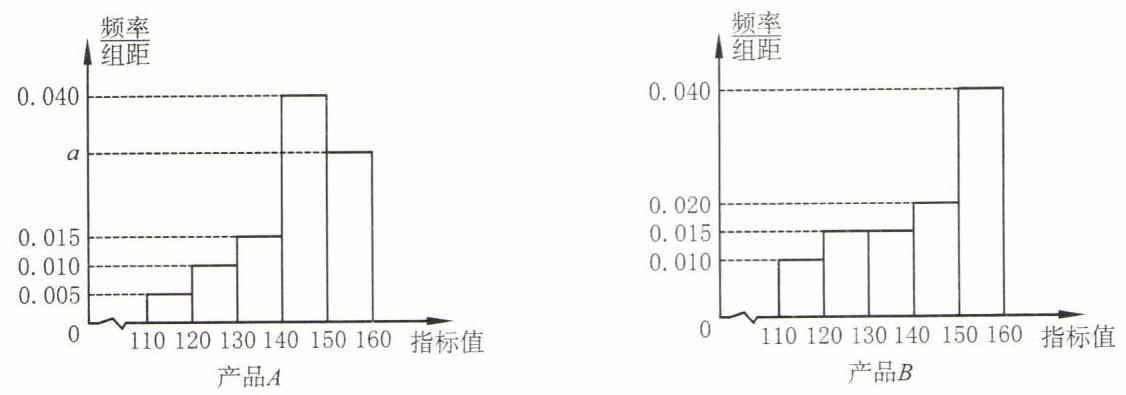
\includegraphics[width=0.9\textwidth]{bodyxb/src/bo_d20aucref24c73anc48g_265_226_1165_1126_395_0.jpg}
\end{center}


(第 91 题)

(注:收益率 $= \dfrac{\text{ 利润 }}{\text{ 总投资额) }}$

\begin{center}
\adjustbox{width=\textwidth}{
\begin{tabular}{|c|c|c|c|}
\hline
等级 & 一等品 & 二等品 & 三等品 \\
\cline{1-4}
指标值 $m$ & $m \geq  {140}$ & ${120} \leq  m < {140}$ & $m < {120}$ \\
\cline{1-4}
产品收益率 & $p$ & $4{p}^{2}$ & ${p}^{2}$ \\
\cline{1-4}
\hline
\end{tabular}
}
\end{center}

(1)求 $a$ 的值；

(2)将频率分布直方图中的频率近似看作概率,并用样本估计总体.

①从产品 $B$ 中随机抽取 3 件,求其中一等品件数 $X$ 的分布及数学期望；

②在总投资额相同的情况下,若全部投资产品 $A$ 或产品 $B$ ,试分析投资哪种产品收益更大.

92. 已知某超市销售的袋装食用盐的质量 $X$ (单位: $\mathrm{g}$ ) 服从正态分布 $N\left( {\mu ,{\sigma }^{2}}\right)$ ,且 $P\left( {X < {249}}\right)$  $= {0.15}$ . 某次该超市称量了 120 袋食用盐,其总质量为 ${30}\mathrm{{kg}},\mu$ 的值恰好等于这 120 袋食用盐每袋的平均质量(单位:g).

(1)若从该超市销售的袋装食用盐中随机选取 2 袋,设这 2 袋中质量不小于 ${250}\mathrm{g}$ 的袋数为 $Z$ ,求 $Z$ 的分布;

(2)若从该超市销售的袋装食用盐中随机选取 $k$ ( $k$ 为正整数) 袋,记质量在 ${249}\mathrm{g} \sim  {251}\mathrm{g}$ 的袋数为 $Y$ ,求满足 $D\left\lbrack  Y\right\rbrack   < {42}$ 的 $k$ 的最大值.

93. 某企业准备投产一批特殊型号的产品,已知该种产品的成本 $C$ 与产量 $q$ 的函数关系为 $C$  $= \dfrac{{q}^{3}}{3} - 3{q}^{2} + {20q} + {10}\left( {q > 0}\right)$ . 该种产品的市场前景无法确定,有三种可能出现的情况,各种情形发生的概率及相应的产品价格 $p$ 与产量 $q$ 的函数关系式如下表所示:

\begin{center}
\adjustbox{width=\textwidth}{
\begin{tabular}{|c|c|c|}
\hline
市场情形 & 概率 & 价格 $p$ 与产量 $q$ 的函数关系式 \\
\cline{1-3}
好 & 0.4 & $p = {164} - {3q}$ \\
\cline{1-3}
中 & 0.4 & $p = {101} - {3q}$ \\
\cline{1-3}
差 & 0.2 & $p = {70} - {3q}$ \\
\cline{1-3}
\hline
\end{tabular}
}
\end{center}

设 ${L}_{1},{L}_{2},{L}_{3}$ 分别表示市场情形好、中、差时的利润,随机变量 ${\xi }_{q}$ 表示当产量为 $q$ ,而市场前景无法确定时的利润.

(1)分别求利润 ${L}_{1},{L}_{2},{L}_{3}$ 与产量 $q$ 的函数关系式；

(2)当产量 $q$ 确定时,求期望 $E\left\lbrack  {\xi }_{q}\right\rbrack$ ；

(3)当产量 $q$ 取何值时,期望 $E\left\lbrack  {\xi }_{q}\right\rbrack$ 取得最大值.

\section*{(B)}

94. 某银行有一自动取款机,在某时刻恰有 $k\left( {k \in  \vv{n}}\right)$ 个人正在使用或等待使用该取款机的概率为 $p\left( k\right)$ . 已知 $p\left( k\right)  = \left\{  \begin{array}{l} {\left( \dfrac{1}{2}\right) }^{k} \cdot  p\left( 0\right) ,0 \leq  k < 5, \\  0,k \geq  5, \end{array}\right.$ 则在该时刻没有人正在使用或等待使用该取款机的概率为(   )

(A) $\dfrac{32}{63}$ . (B) $\dfrac{16}{31}$ . (C) $\dfrac{8}{15}$ . (D) $\dfrac{4}{7}$ .

95. 我们将服从二项分布的随机变量称为二项随机变量, 服从正态分布的随机变量称为正态随机变量. 概率论中有一个重要的结论: 若随机变量 $Y \sim  B\left( {n,p}\right)$ ,当 $n$ 充分大时,二项随机变量 $Y$ 可以由正态随机变量 $X$ 来近似地替代,且正态随机变量 $X$ 的期望和方差与二项随机变量 $Y$ 的期望和方差相同. 法国数学家棣莫弗(1667 - 1754)在 1733 年证明了 $p = \dfrac{1}{2}$ 时这个结论是成立的；法国数学家、物理学家拉普拉斯(1749-1827)在 1812 年证明了这个结论对任意的实数 $p \in  \left( {0,1}\right)$ 都成立,因此人们把这个结论称为棣莫弗一拉普拉斯极限定理. 现抛掷一枚质地均匀的硬币 2500 次, 利用正态分布估算硬币正面向上的次数不少于

1 200 次的概率为(   )

参考数据: $P\left( {\mu  - \sigma  \leq  X \leq  \mu  + \sigma }\right)  \approx  {0.6826},P\left( {\mu  - {2\sigma } \leq  X \leq  \mu  + {2\sigma }}\right)  \approx  {0.9544},P(\mu  - {3\sigma } \leq$  $X \leq  \mu  + {3\sigma }) \approx  {0.9974}$ .

(A) 0.9987 . (B) 0.9772 .

(C) 0.8413 . (D) 0.6586 .

96. 现有甲、乙两个盒子,甲盒有 1 个红球,乙盒有 3 个红球和 3 个黑球,现从乙盒里随机取出 $n\left( {1 \leq  n \leq  6,n \in  \vv{n}}\right)$ 个球放入甲盒后,再从甲盒里随机取一球,记取到的红球个数为 $\xi$ ,则随着 $n\left( {1 \leq  n \leq  6,n \in  \vv{n}}\right)$ 的增加,下列说法正确的是 (   )

(A) $E\left\lbrack  \xi \right\rbrack$ 增加, $D\left\lbrack  \xi \right\rbrack$ 增加. (B) $E\left\lbrack  \xi \right\rbrack$ 增加, $D\left\lbrack  \xi \right\rbrack$ 减小.

(C) $E\left\lbrack  \xi \right\rbrack$ 减小, $D\left\lbrack  \xi \right\rbrack$ 增加. (D) $E\left\lbrack  \xi \right\rbrack$ 减小, $D\left\lbrack  \xi \right\rbrack$ 减小.

97. 盲拧魔方游戏,就是玩家先观察魔方状态并进行记忆,记住后蒙住眼睛快速还原魔方. 为了解某市盲拧魔方爱好者的水平状况,某兴趣小组在全市范围内随机抽取了 100 名盲拧魔方爱好者进行调查,得到的情况如表所示:

\begin{center}
\adjustbox{width=\textwidth}{
\begin{tabular}{|c|c|c|c|c|}
\hline
用时/秒 & $\left\lbrack  {5,{10}}\right\rbrack$ & (10,15) & (15,20) & $\left( {{20},{25}}\right\rbrack$ \\
\cline{1-5}
男性人数 & 17 & 21 & 13 & 9 \\
\cline{1-5}
女性人数 & 8 & 10 & 16 & 6 \\
\cline{1-5}
\hline
\end{tabular}
}
\end{center}

以这 100 名盲拧魔方爱好者用时不超过 10 秒的频率,近似估计全市所有盲拧魔方爱好者用时不超过 10 秒的概率,且每位盲拧魔方爱好者用时是否超过 10 秒相互独立. 若该兴趣小组在全市范围内再随机抽取 20 名盲拧魔方爱好者进行测试, 其中用时不超过 10 秒的人数最有可能(即概率最大)是(   )

(A) 3 . (B) 4. (C) 5. (D) 6.

98. 已知随机变量 $\xi  \sim  N\left( {\mu ,{\sigma }^{2}}\right)$ ,设函数 $f\left( x\right)  = P\left( {\xi  \geq  x + 2}\right)$ ,且 $f\left( x\right)$ 满足 $f\left( x\right)  + f\left( {-x}\right)  =$ 1,则 $\mu  =$ \blkda{}.

99. 某保险公司新开设了一项保险业务,若在一年内事件 $E$ 发生,该公司要赔偿 $a$ 元. 设在一年内事件 $E$ 发生的概率为 $1\%$ ,为使公司收益的期望值等于 ${0.1a}$ ,公司应要求顾客交保险金为\blkda{}元. (用含 $a$ 的代数式表示)

100. 某种植户对一块地的 $n$ 个坑进行播种,每个坑播 3 粒种子,每粒种子发芽的概率均为 $\dfrac{1}{2}$ ,且每粒种子是否发芽相互独立. 对每个坑而言, 如果至少有两粒种子发芽, 则不需要进行补播种, 否则要补播种. 当 $n =$ \blkda{}时,有 3 个坑要补播种的概率最大,最大概率为\blkda{}.

101. 已知甲、乙两支队伍中各有 20 人,甲队中有 $x\left( {0 < x < {20}}\right)$ 名男生与 ${20} - x$ 名女生,乙队伍中有 ${20} - x$ 名男生与 $x$ 名女生. 若从甲、乙两队中各选 1 人, $X$ 表示所选的 2 人中男生的人数,则当方差 $D\left\lbrack  X\right\rbrack$ 取到最大值时, $x$ 的值为\blkda{}.

102. 假设某型号的飞机的引擎在飞行中出现故障的概率为 $1 - p\left( {0 < p < 1}\right)$ ,且各引擎是否发生故障相互独立,若有至少 ${50}\%$ 的引擎能正常运行,飞机就可成功飞行. 若四个引擎的飞机比两个引擎的飞机更为安全,则 $p$ 的取值范围是\blkda{}.

103. 某学生在上学路上要经过三个路口,且在各个路口遇到红灯的概率及停留的时间如下:

\begin{center}
\adjustbox{width=\textwidth}{
\begin{tabular}{|c|c|c|c|}
\hline
路口 & 一 & 二 & 三 \\
\cline{1-4}
遇到红灯的概率 & $\dfrac{1}{4}$ & $\dfrac{1}{3}$ & $\dfrac{1}{2}$ \\
\cline{1-4}
遇到红灯停留的时间 & 3 分钟 & 2 分钟 & 1 分钟 \\
\cline{1-4}
\hline
\end{tabular}
}
\end{center}

假设在各路口是否遇到红灯相互独立.

(1)求这名学生在上学路上到第三个路口时首次遇到红灯的概率；

(2)求这名学生在上学路上因遇到红灯停留的总时间大于 3 分钟的概率；

(3)假设交管部门根据实际路况,5 月 1 日之后将上述三个路口遇到红灯停留的时间都变为 2 分钟. 试估计 5 月 1 日之后这名学生在上学路上因遇到红灯停留的总时间的变化情况, 是增加、不变还是减少.

104. 马尔科夫链是概率统计中的一个重要模型, 也是机器学习和人工智能的基石. 马尔科夫过程要求具备“无记忆”的性质, 即下一状态的概率分布只能由当前状态决定, 在时间序列中前面的事件均与之无关. 已知甲、乙两口袋中各装有 1 个黑球和 2 个白球, 现从甲、乙两口袋中各任取一个球交换放入另一口袋,重复进行 $n\left( {n \in  \vv{n},n \geq  1}\right)$ 次这样的操作,记甲口袋中黑球的个数为 ${X}_{n}$ ,且甲口袋中恰有 1 个黑球的概率为 ${p}_{n}$ .

(1) 求 ${p}_{1},{p}_{2}$ 的值;

(2) 求 ${p}_{n}$ 的值 (用 $n$ 表示);

(3) 求证: ${X}_{n}$ 的数学期望 $E\left\lbrack  {X}_{n}\right\rbrack$ 为定值.

105. 工作人员需进入核电站完成某项具有高辐射危险的任务,每次只派一人进去,且每人只派一次,工作时间不超过 10 分钟,如果有一人 10 分钟内不能完成任务则撤出,再派下一人. 现在一共只有甲、乙、丙三人可派,他们各自能完成任务的概率分别 ${p}_{1},{p}_{2},{p}_{3}$ ,假设 ${p}_{1},{p}_{2},{p}_{3}$ 互不相等,且假定各人能否完成任务的事件相互独立.

(1)如果按甲在先,乙次之,丙最后的顺序派人,求任务能被完成的概率. 若改变三人被派出的先后顺序,任务能被完成的概率是否发生变化?

(2)若按某指定顺序派人,这三人各自能完成任务的概率依次为 ${q}_{1},{q}_{2},{q}_{3}$ ,其中 ${q}_{1},{q}_{2}$ , ${q}_{3}$ 是 ${p}_{1},{p}_{2},{p}_{3}$ 的一个排列,求所需派出人员数目 $X$ 的分布和期望;

(3)假定 $1 > {p}_{1} > {p}_{2} > {p}_{3}$ ,试分析以怎样的先后顺序派出人员,可使所需派出的人员数目的均值 (数学期望) 达到最小.

106. 某车间用一台包装机包装葡萄糖,每袋葡萄糖的重量是一个随机变量,它服从正态分布. 当机器工作正常时,每袋葡萄糖平均重量 ${\mu }_{0}$ 为 ${0.5}\mathrm{{kg}}$ ,标准差 $\sigma$ 为 ${0.015}\mathrm{{kg}}$ .

(1)已知包装每袋葡萄糖的成本为 1 元,若发现包装好的葡萄糖重量异常,则需要将该袋葡萄糖进行重新包装,假设重新包装后的葡萄糖重量正常. 若某袋葡萄糖的重量 ${m}_{0}$ 满足 ${\mu }_{0} - \sigma  < {m}_{0} < {\mu }_{0} + \sigma$ ,则认为该袋葡萄糖重量正常. 问: 在机器工作正常的情况下, 至少包装多少袋葡萄糖才能使 “至少有一袋包装好的葡萄糖重量正常” 的概率大于 0.98 ? 并求出相应成本的最小期望值；

(2)某日开工后,为检查该包装机工作是否正常,随机地抽取它所包装的葡萄糖 9 袋,若抽取的 9 袋葡萄糖称得净重(kg)为:0.496,0.508,0.524,0.519,0.495,0.510, 0.522,0.513,0.512. 用样本平均数 $\bar{x}$ 作为 $\mu$ 的估计值 $\widehat{\mu }$ ,用样本标准差 $S$ 作为 $\delta$ 的估计值 $\widehat{\delta }$ ,以 $\left| Z\right|  = \left| \dfrac{\widehat{\mu } - {\mu }_{0}}{\dfrac{\sigma }{\sqrt{n}}}\right|$ 作为检验统计量,其中 $n$ 为样本总数, $Z$ 服从正态分布 $Z \sim  N\left( {0,1}\right)$ ,且 $P\left( {-{1.96} < Z < {1.96}}\right)  \approx  {0.95}$ .

①若机器工作正常时,每袋葡萄糖的重量服从的正态分布曲线如右图所示, 请在右图 (机器正常工作时的正态分布曲线)中,绘制出以该样本作为估计得到的每袋葡萄糖所服从的正态分布曲线的草图;

\begin{center}
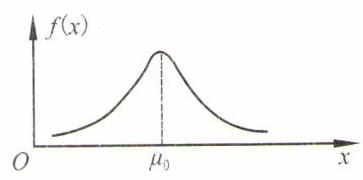
\includegraphics[width=0.3\textwidth]{bodyxb/src/bo_d20aucref24c73anc48g_269_1062_501_363_180_0.jpg}
\end{center}


(第 106 题)

②若 $P\left( {\left| Z\right|  \geq  k}\right)  = a\left( {0 < a < 1}\right)$ ,就推断该包装机工作异常,这种推断犯错误的概率不超过 $a$ . 试在犯错概率不超过 0.05 的前提下,估计该包装机工作是否正常.

参考数据: 若随机变量 $Z$ 服从正态分布: $P\left( {\mu  - \sigma  < Z < \mu  + \sigma }\right)  = {0.6826}$ ,

$P\left( {\mu  - {2\sigma } < Z < \mu  + {2\sigma }}\right)  = {0.9544},P\left( {\mu  - {3\sigma } < Z < \mu  + {3\sigma }}\right)  = {0.9974}.$

\section*{四、成对数据的统计分析}

\section*{【典型题型和解题技巧】}

例 1 随着快递业的发展,网购的流行,居民不出门通过网购就可以实现轻松购物,为了研究一般家庭月平均收入与月平均网购支出的关系, 某市统计部门随机调查了 10 个有网购经历的家庭,得到数据如下:

\begin{center}
\adjustbox{width=\textwidth}{
\begin{tabular}{|c|c|c|c|c|c|c|c|c|c|c|}
\hline
家庭编号 & 1 & 2 & 3 & 4 & 5 & 6 & 7 & 8 & 9 & 10 \\
\cline{1-11}
${x}_{i}$ (收入)/千元 & 2 & 3 & 4 & 5 & 6 & 7 & 8 & 9 & 10 & 11 \\
\cline{1-11}
${y}_{i}$ (网购支出)/千元 & 0.1 & 0.3 & 0.4 & 0.5 & 0.6 & 0.8 & 1.0 & 1.2 & 1.4 & 1. 6 \\
\cline{1-11}
\hline
\end{tabular}
}
\end{center}

根据表中数据绘制散点图,计算相关系数并判断家庭月平均收入与月平均网购支出的相关程度.

解 绘制的散点图如下:

\begin{center}
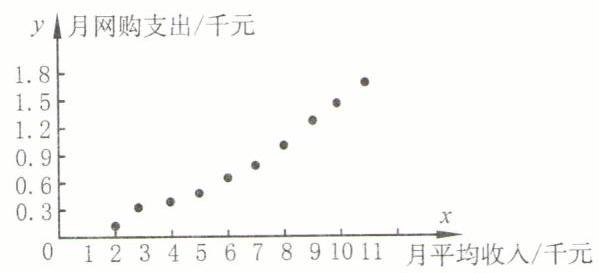
\includegraphics[width=0.5\textwidth]{bodyxb/src/bo_d20aucref24c73anc48g_269_456_1831_599_273_0.jpg}
\end{center}


从图中可以看出, 总体上来说, 各个数据对应的点都在一条直线附近波动, 所以两者呈线性相关关系.

将表中的两组数据代入公式,或者通过计算器,可以得到 $r \approx  {0.992}$ ,所以家庭月平均收入与月平均网购支出具有很强的线性相关关系.

注意 判断两个变量是否具有线性相关关系, 一般有两种办法:

(1)绘制散点图,若从整体上看,所有点都在一条直线的附近波动,则说明这两个变量之间具有线性相关关系, 此时可以通过一条直线来拟合这两组数据.

(2)求线性相关系数 $r$ (也称为皮尔逊相关系数), $\left| r\right|$ 越接近 1,这两个变量的线性相关程度越高.

例 2 食品加工厂新研制出一种袋装食品(规格:500 g/袋),下面是近六个月每袋出厂价格(单位:元)与销售量(单位:万袋)的对应关系表:

\begin{center}
\adjustbox{width=\textwidth}{
\begin{tabular}{|c|c|c|c|c|c|c|}
\hline
月份序号 & 1 & 2 & 3 & 4 & 5 & 6 \\
\cline{1-7}
每袋出厂价格 ${x}_{i}$ & 10.5 & 10.9 & 11 & 11. 5 & 12 & 12.5 \\
\cline{1-7}
月销售量 ${y}_{i}$ & 2.2 & 2 & 1.9 & 1.8 & 1.5 & 1.4 \\
\cline{1-7}
\hline
\end{tabular}
}
\end{center}

经计算得 $\mathop{\sum }\limits_{{i = 1}}^{6}{x}_{i}^{2} = {782.56},\mathop{\sum }\limits_{{i = 1}}^{6}{y}_{i}^{2} = {19.9},\mathop{\sum }\limits_{{i = 1}}^{6}{x}_{i}{y}_{i} = {122}$ .

(1)计算该食品加工厂这六个月内这种袋装食品的平均每袋出厂价格、平均月销售量和平均月销售收入;

(2)求每袋出厂价格与月销售量的样本相关系数(精确到 0.01)；

(3)若样本相关系数 $\left| r\right|  \geq  {0.75}$ ,则认为相关性很强；否则没有较强的相关性. 你认为该食品加工厂制定的每袋食品的出厂价格与月销售量是否有较强的相关性.

解(1)该食品加工厂这六个月内这种袋装食品的平均每袋出厂价格:

$\bar{x} = \dfrac{1}{6} \times  \left( {{10.5} + {10.9} + {11} + {11.5} + {12} + {12.5}}\right)  = {11.4}$ (元),

平均月销售量为 $\bar{y} = \dfrac{1}{6} \times  \left( {{2.2} + 2 + {1.9} + {1.8} + {1.5} + {1.4}}\right)  = {1.8}$ (万袋),

平均月销售收入为 $\dfrac{1}{6}\mathop{\sum }\limits_{{i = 1}}^{6}{x}_{i}{y}_{i} = \dfrac{1}{6} \times  {122} = \dfrac{61}{3}$ (万元).

(2)由已知,每袋出厂价格与月销售量的样本相关系数:

$r = \dfrac{\mathop{\sum }\limits_{{i = 1}}^{6}{x}_{i}{y}_{i} - 6\bar{x} \cdot  \bar{y}}{\sqrt{\left( {\mathop{\sum }\limits_{{i = 1}}^{6}{x}_{i}^{2} - 6{\bar{x}}^{2}}\right) \left( {\mathop{\sum }\limits_{{i = 1}}^{6}{y}_{i}^{2} - 6{\bar{y}}^{2}}\right) }} \approx   - {0.99}$

(3)由于 $\left| r\right|  \approx  {0.99} > {0.75}$ ,所以该食品加工厂制定的每袋食品的出厂价格与月销售量有较强的相关性.

注意 相关系数 $r$ 的计算公式:

\[
r = \dfrac{\mathop{\sum }\limits_{{i = 1}}^{n}\left( {{x}_{i} - \bar{x}}\right) \left( {{y}_{i} - \bar{y}}\right) }{\sqrt{\mathop{\sum }\limits_{{i = 1}}^{n}{\left( {x}_{i} - \bar{x}\right) }^{2}}\sqrt{\mathop{\sum }\limits_{{i = 1}}^{n}{\left( {y}_{i} - \bar{y}\right) }^{2}}} = \dfrac{\mathop{\sum }\limits_{{i = 1}}^{n}{x}_{i}{y}_{i} - n\bar{x} \cdot  \bar{y}}{\sqrt{\left( {\mathop{\sum }\limits_{{i = 1}}^{n}{x}_{i}^{2} - n{\bar{x}}^{2}}\right) \left( {\mathop{\sum }\limits_{{i = 1}}^{n}{y}_{i}^{2} - n{\bar{y}}^{2}}\right) }}
\]

(其中 ${x}_{1},{x}_{2},\cdots ,{x}_{n}$ 和 ${y}_{1},{y}_{2},\cdots ,{y}_{n}$ 的均值分别为 $\bar{x}$ 和 $\overline{{y}^{\prime }}$ ).

当 $r > 0$ 时,称这种相关为正相关; 当 $r < 0$ 时,称这种相关为负相关.

例 3 某调查机构分析发现公司员工的身高 $x\left( \mathrm{{cm}}\right)$ 和体重 $y\left( \mathrm{{kg}}\right)$ 之间有较强的线性相关关系,调查员甲对其中 8 名员工的体检数据进行分析,计算得到线性回归方程为 $y = {0.5x} + \widehat{b}$ , 并根据回归方程预测一名身高为 ${180}\mathrm{{cm}}$ 的员工体重为 ${71}\mathrm{{kg}}$ . 计算得到的其他数据如下: $\bar{x} =$  ${170},\mathop{\sum }\limits_{{i = 1}}^{8}{x}_{i}{y}_{i} = {89920}$

(1)求 $\widehat{b}$ 的值及抽取的 8 人体重数据的平均值 $\bar{y}$ ；

(2)调查员乙代替甲继续数据处理时,发现编号为 8 的员工体重数据有误,应增加 8 kg, 其身高数据 ${182}\mathrm{{cm}}$ 无误,请你根据调查员乙更正的数据重新计算线性回归方程,并据此预测一名身高为 ${180}\mathrm{{cm}}$ 的员工的体重.

参考公式: 对于一组具有线性相关关系的数据 $\left( {{x}_{i},{y}_{i}}\right) \left( {i = 1,2,3,\cdots ,n}\right)$ ,其回归直线 $y =$  $\widehat{a}x + \widehat{b}$ 的斜率和截距的最小二乘估计公式分别为

\[
\widehat{a} = \dfrac{\mathop{\sum }\limits_{{i = 1}}^{n}\left( {{x}_{i} - \bar{x}}\right) \left( {{y}_{i} - \bar{y}}\right) }{\mathop{\sum }\limits_{{i = 1}}^{n}{\left( {x}_{i} - \bar{x}\right) }^{2}} = \dfrac{\mathop{\sum }\limits_{{i = 1}}^{n}{x}_{i}{y}_{i} - n\bar{x}\bar{y}}{\mathop{\sum }\limits_{{i = 1}}^{n}{x}_{i}^{2} - n{\bar{x}}^{2}},\widehat{b} = \bar{y} - \widehat{a}\bar{x}.
\]

解(1)因为根据回归方程的预估,一名身高为 ${180}\mathrm{{cm}}$ 的员工的体重为 ${71}\mathrm{{kg}}$ ,

所以 ${71} = {0.5} \times  {180} + \widehat{b}$ ,可得 $\widehat{b} =  - {19}$ ,所以线性回归方程为 $y = {0.5x} - {19}$ .

因为样本中心 $\left( {\bar{x},\bar{y}}\right)$ 一定在回归直线 $y = {0.5x} - {19}$ 上,可得 $\bar{y} = {0.5} \times  {170} - {19} = {66}$ .

( 2 )由( 1 )知更正前的数据为 $\bar{x} = {170},\bar{y} = {66}$ .

因为 $\widehat{a} = \dfrac{\mathop{\sum }\limits_{{i = 1}}^{n}{x}_{i}{y}_{i} - n\bar{x}\bar{y}}{\mathop{\sum }\limits_{{i = 1}}^{n}{x}_{i}^{2} - n{\bar{x}}^{2}} = \dfrac{\mathop{\sum }\limits_{{i = 1}}^{8}{x}_{i}{y}_{i} - 8\bar{x}\bar{y}}{\mathop{\sum }\limits_{{i = 1}}^{8}{x}_{i}^{2} - 8{\bar{x}}^{2}} = {0.5}$ ,所以 $\mathop{\sum }\limits_{{i = 1}}^{8}{x}_{i}^{2} - 8{\bar{x}}^{2} = {320}$ .

更正后的数据为 $\overline{{x}^{\prime }} = \overline{x} = {170},\overline{{y}^{\prime }} = \dfrac{{66} \times  8 + 8}{8} = {67}$ ,

所以 $\mathop{\sum }\limits_{{i = 1}}^{8}{x}_{i}^{\prime }{y}_{i}^{\prime } = \mathop{\sum }\limits_{{i = 1}}^{8}{x}_{i}{y}_{i} + {x}_{8} \times  8 = \mathop{\sum }\limits_{{i = 1}}^{8}{x}_{i}{y}_{i} + {182} \times  8,8\overline{{x}^{\prime }{y}^{\prime }} = 8\bar{x}\left( {\bar{y} + 1}\right)  = 8\bar{x}\bar{y} + 8 \times  {170}$ ,

所以 $\widehat{{a}^{\prime }} = \dfrac{\mathop{\sum }\limits_{{i = 1}}^{n}{x}_{i}^{\prime }{y}_{i}^{\prime } - n\overline{{x}^{\prime }{y}^{\prime }}}{\mathop{\sum }\limits_{{i = 1}}^{n}{x}_{i}^{\prime 2} - n\overline{{x}^{\prime 2}}} = \dfrac{\left( {\mathop{\sum }\limits_{{i = 1}}^{8}{x}_{i}{y}_{i} + {182} \times  8}\right)  - \left( {8\bar{x}\bar{y} + 8 \times  {170}}\right) }{\mathop{\sum }\limits_{{i = 1}}^{8}{x}_{i}^{2} - 8{\bar{x}}^{2}} = {0.8}$ ,

所以 ${\widehat{b}}^{\prime } = \overline{{y}^{\prime }} - {\widehat{a}}^{\prime }\overline{{x}^{\prime }} = {67} - {0.8} \times  {170} =  - {69}$ .

故更正后的线性回归方程为 $y = {0.8x} - {69}$ ,

当 $x = {180}$ 时,可得 $y = {0.8} \times  {180} - {69} = {75}$ ,

所以重新预估一名身高为 ${180}\mathrm{{cm}}$ 的员工的体重为 ${75}\mathrm{{kg}}$ .

注意 一元线性回归模型参数的最小二乘估计.

(1)经验回归直线.

如果散点图中点的分布从整体上看大致在一条直线附近, 则称这两个变量之间具有线性相关关系,且将 $y = \widehat{a}x + \widehat{b}$ 称为 $y$ 随 $x$ 波动的回归方程,回归方程所定义的直线称为回归直线.

(2)最小二乘估计.

求回归方程 $y = \widehat{a}x + \widehat{b}$ 时,使得样本数据点到回归直线的竖直距离的平方之和 (即离差的平方和) 最小的方法叫最小二乘法. 求得的 $\widehat{a},\widehat{b}$ 叫 $a,b$ 的最小二乘估计.

\[
\widehat{a} = \dfrac{\mathop{\sum }\limits_{{i = 1}}^{n}\left( {{x}_{i} - \bar{x}}\right) \left( {{y}_{i} - \bar{y}}\right) }{\mathop{\sum }\limits_{{i = 1}}^{n}{\left( {x}_{i} - \bar{x}\right) }^{2}} = \dfrac{\mathop{\sum }\limits_{{i = 1}}^{n}{x}_{i}{y}_{i} - n\bar{x}\bar{y}}{\mathop{\sum }\limits_{{i = 1}}^{n}{x}_{i}^{2} - n{\bar{x}}^{2}},\widehat{b} = \bar{y} - \widehat{a}\bar{x}.
\]

$\widehat{a}$ 与 $\widehat{b}$ 称为回归系数. 回归直线一定经过样本点的中心 $\left( {\bar{x},\bar{y}}\right)$ .

例 4 下表中是统计学家安斯库姆(F. Anscombe)所提供的 4 组数据. 这四组数据的线性相关系数非常接近,均约等于 0.816 ,如果对它们作线性回归分析,得到的线性回归方程也基本一致,均可表示为 $y = 3 + {0.5x}$ .

数据组 $A$

\begin{center}
\adjustbox{width=\textwidth}{
\begin{tabular}{|c|c|c|c|c|c|c|c|c|c|c|c|}
\hline
$x$ & 10 & 8 & 13 & 9 & 11 & 14 & 6 & 4 & 12 & 7 & 5 \\
\cline{1-12}
$y$ & 8.04 & 6.95 & 7.58 & 8. 81 & 8.33 & 9.96 & 7.24 & 4. 26 & 10.84 & 4.82 & 5. 68 \\
\cline{1-12}
\hline
\end{tabular}
}
\end{center}

数据组 $B$ 数据组 $C$

\begin{center}
\adjustbox{width=\textwidth}{
\begin{tabular}{|c|c|c|c|c|c|c|c|c|c|c|c|}
\hline
$x$ & 10 & 8 & 13 & 9 & 11 & 14 & 6 & 4 & 12 & 7 & 5 \\
\cline{1-12}
$y$ & 9. 14 & 8. 14 & 8.74 & 8. 77 & 9.26 & 8. 10 & 6.13 & 3.10 & 9.13 & 7.26 & 4. 74 \\
\cline{1-12}
\hline
\end{tabular}
}
\end{center}

\begin{center}
\adjustbox{width=\textwidth}{
\begin{tabular}{|c|c|c|c|c|c|c|c|c|c|c|c|}
\hline
$x$ & 10 & 8 & 13 & 9 & 11 & 14 & 6 & 4 & 12 & 7 & 5 \\
\cline{1-12}
$y$ & 7.46 & 6.77 & 12.74 & 7. 11 & 7.81 & 8.84 & 6.08 & 5.39 & 8. 15 & 6.42 & 5.73 \\
\cline{1-12}
\hline
\end{tabular}
}
\end{center}

数据组 $D$

\begin{center}
\adjustbox{width=\textwidth}{
\begin{tabular}{|c|c|c|c|c|c|c|c|c|c|c|c|}
\hline
$x$ & 8 & 8 & 8 & 8 & 8 & 8 & 8 & 8 & 8 & 8 & 19 \\
\cline{1-12}
$y$ & 6. 58 & 5.76 & 7.71 & 8.84 & 8.47 & 7.04 & 5.25 & 5.56 & 7. 91 & 6.89 & 12.50 \\
\cline{1-12}
\hline
\end{tabular}
}
\end{center}

(1)这四组数据的线性相关程度真的如此一致吗？

(2)对哪个(些)组的数据,可以用回归直线来预测 $x = {10}$ 时的 $y$ 值？

( 3 )分别对四组数据提出自己的见解.

解(1)数据组 $A$ 对应的散点图及直线 $y = {0.5x} + 3$ 如下:

\begin{center}
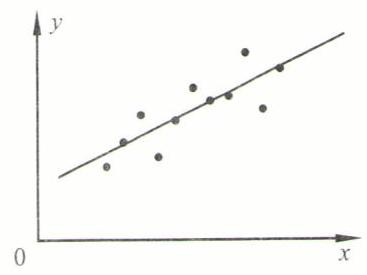
\includegraphics[width=0.3\textwidth]{bodyxb/src/bo_d20aucref24c73anc48g_272_686_1785_367_275_0.jpg}
\end{center}


数据组 $B$ 对应的散点图及直线 $y = {0.5x} + 3$ 如下:

\begin{center}
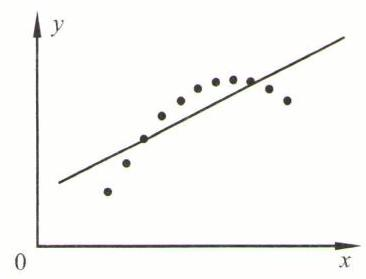
\includegraphics[width=0.3\textwidth]{bodyxb/src/bo_d20aucref24c73anc48g_273_558_201_366_279_0.jpg}
\end{center}


数据组 $C$ 对应的散点图及直线 $y = {0.5x} + 3$ 如下:

\begin{center}
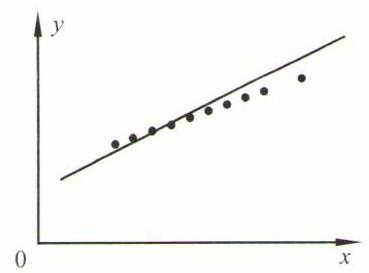
\includegraphics[width=0.3\textwidth]{bodyxb/src/bo_d20aucref24c73anc48g_273_558_539_369_273_0.jpg}
\end{center}


数据组 $D$ 对应的散点图及直线 $y = {0.5x} + 3$ 如下:

\begin{center}
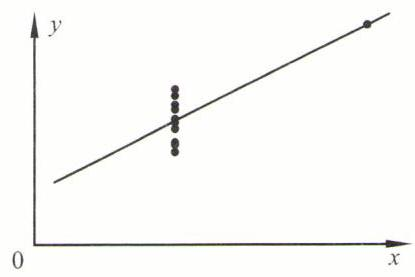
\includegraphics[width=0.3\textwidth]{bodyxb/src/bo_d20aucref24c73anc48g_273_535_872_415_277_0.jpg}
\end{center}


由以上散点图知: 四组数据的线性相关程度并不一致.

(2)由(1)可知:数据组 $C$ 中的数据点更贴近回归直线,故用它来预测 $x = {10}$ 时的 $y$ 值.

(3)①相关系数接近且回归直线一致,并不能保证数据样本之间的线性相关程度一致；

②数据分析前需要对原始数据进行作图分析,如果相关变量的关系是非线性的,而分析过程中应用线性方程拟合, 会导致分析结果与实际结果有很大的差异.

注意 这个例子表明,对于一组数据建立一元线性回归模型的基本前提是,自变量与因变量之间需存在线性关系,这也是初学者往往容易忽视的地方.

例 5 随着全球新能源汽车市场蓬勃增长, 在政策推动下, 中国新能源汽车企业在 10 余年间实现了“弯道超车”,一跃成为新能源汽车产量连续 7 年居世界第一的全球新能源汽车强国. 某新能源汽车企业基于领先技术的支持,改进并生产纯电动车、插电混合式电动车、氢燃料电动车三种车型, 生产效益在短期内逐月攀升, 现根据该企业在 1 月份至 6 月份的生产利润 $y$ (单位: 百万元) 关于月份 $x$ 的数据,绘制了如图所示的散点图.

\begin{center}
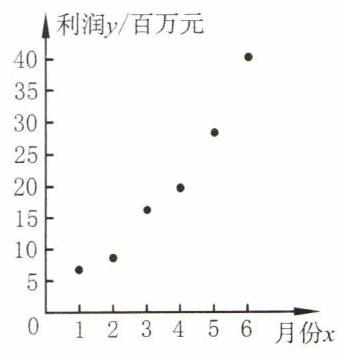
\includegraphics[width=0.2\textwidth]{bodyxb/src/bo_d20aucref24c73anc48g_273_1078_1546_345_354_0.jpg}
\end{center}


(1)根据散点图判断, $y = {ax} + b$ 与 $y = c{\mathrm{e}}^{dx}$ ( $a,b,c,d$ 均为常数) 哪一个更适宜作为利润 $y$ 关于月份 $x$ 的回归方程类型? (给出判断即可,不必说明理由)

(2)根据(1)的结果及表中的数据,求出 $y$ 关于 $x$ 的回归方程.

提示: 设 $u = \ln y,{u}_{i} - \ln {y}_{i}\left( {i - 1,2,3,4,5,6}\right)$ . 参考数据:

\begin{center}
\adjustbox{width=\textwidth}{
\begin{tabular}{|c|c|c|c|c|}
\hline
$\bar{y}$ & $\bar{u}$ & $\mathop{\sum }\limits_{{i = 1}}^{6}{\left( {x}_{i} - \bar{x}\right) }^{2}$ & $\mathop{\sum }\limits_{{i = 1}}^{6}\left( {{x}_{i} - \bar{x}}\right) \left( {{y}_{i} - \bar{y}}\right)$ & $\mathop{\sum }\limits_{{i = 1}}^{6}\left( {{x}_{i} - \bar{x}}\right) \left( {{u}_{i} - \bar{u}}\right)$ \\
\cline{1-5}
19.87 & 2.80 & 17.50 & 113.75 & 6.30 \\
\cline{1-5}
\hline
\end{tabular}
}
\end{center}

参考公式: 对于一组具有线性相关关系的数据 $\left( {{x}_{i},{y}_{i}}\right) \left( {i = 1,2,3,\cdots ,n}\right)$ ,其回归直线 $y =$  $\widehat{a}x + \widehat{b}$ 的斜率和截距的最小二乘估计公式分别为

\[
\widehat{a} = \dfrac{\mathop{\sum }\limits_{{i = 1}}^{n}\left( {{x}_{i} - \bar{x}}\right) \left( {{y}_{i} - \bar{y}}\right) }{\mathop{\sum }\limits_{{i = 1}}^{n}{\left( {x}_{i} - \bar{x}\right) }^{2}} = \dfrac{\mathop{\sum }\limits_{{i = 1}}^{n}{x}_{i}{y}_{i} - n\bar{x}\bar{y}}{\mathop{\sum }\limits_{{i = 1}}^{n}{x}_{i}^{2} - n{\bar{x}}^{2}},\widehat{b} = \bar{y} - \widehat{a}\bar{x}.
\]

解(1)选用 $y = c{\mathrm{e}}^{dx}$ 作为利润 $y$ 关于月份 $x$ 的回归方程更合适.

(2)由 $y = c{\mathrm{e}}^{dx}$ ,取对数可得 $\ln y = \ln c + {dx}$ ,设 $u = \ln y$ ,所以 $u = {dx} + \ln c$ ,

$\bar{x} = \dfrac{1 + 2 + 3 + 4 + 5 + 6}{6} = {3.5},\mathop{\sum }\limits_{{i = 1}}^{6}{\left( {x}_{i} - \bar{x}\right) }^{2} = {17.50},\mathop{\sum }\limits_{{i = 1}}^{6}\left( {{x}_{i} - \bar{x}}\right) \left( {{u}_{i} - \bar{u}}\right)  = {6.30}$ ,

$\bar{u} = {2.80}$ ,所以 $d = \dfrac{\mathop{\sum }\limits_{{i = 1}}^{6}\left( {{x}_{i} - \bar{x}}\right) \left( {{u}_{i} - \bar{u}}\right) }{\mathop{\sum }\limits_{{i = 1}}^{6}{\left( {x}_{i} - \bar{x}\right) }^{2}} = \dfrac{6.30}{17.5} = {0.36},{2.80} = {0.36} \times  {3.5} + \ln c$ ,

所以 $\ln c = {2.80} - {0.36} \times  {3.5} = {1.54},\ln y = {0.36x} + {1.54}$ ,即 $y = {\mathrm{e}}^{1.54}{\mathrm{e}}^{0.36x}$ .

注意 非线性回归问题有时候并没有给出经验公式, 此时往往需要根据已知数据绘制散点图或利用已知散点图,并根据散点图选择恰当的拟合函数,然后再利用变量代换,将非线性回归问题转化为线性回归问题加以解决. 常见非线性回归方程的转换方式有:

① $y = a{x}^{b}\left( {a > 0}\right)$ ,令 $u = \ln y,v = \ln x$ ,则 $u = \ln a + {bv}$ ；

② $y = a{\mathrm{e}}^{bx}\left( {a > 0}\right)$ ,令 $u = \ln y$ ,则 $u = \ln a + {bx}$ ；

③ $y = a{\mathrm{e}}^{\dfrac{b}{x}}\left( {a > 0}\right)$ ,令 $u = \ln y,v = \dfrac{1}{x}$ ,则 $u = \ln a + {bv}$ ;

④ $y = a + b\ln x$ ,令 $v = \ln x$ ,则 $y = a + {bv}$ .

例 6 通常人们认为语文作文成绩与课外阅读习惯(阅读习惯分为良好和不够良好两类) 有很大关联,为了研究这个看法是否可信,某课外研究小组从学校一次期中测试语文作文成绩优秀的学生中随机调查了 200 人,同时在语文作文成绩不够优秀的学生中也随机调查了 200 人,得到如下数据:

\begin{center}
\adjustbox{width=\textwidth}{
\begin{tabular}{|c|c|c|c|}
\hline
\multirow{2}{*}{语文作文成绩} & \multicolumn{2}{|c|}{课外阅读习惯} & \multirow{2}{*}{合计} \\
\cline{2-3}
 & 不够良好 & 良好 &  \\
\cline{1-4}
优秀 & 60 & 140 & 200 \\
\cline{1-4}
不够优秀 & 180 & 20 & 200 \\
\cline{1-4}
合计 & 240 & 160 & 400 \\
\cline{1-4}
\hline
\end{tabular}
}
\end{center}

(1)在这 400 名学生中按照课外阅读习惯良好与否进行分层随机抽样,抽取 20 名学生了解学生的行为习惯形成的原因,再从这 20 名学生中任选 3 人进行面对面访谈,求这 3 名学生中至少有 1 人课外阅读习惯良好的概率;

(2)根据小概率值 $\alpha  = {0.001}$ 的独立性检验,能否认为语文作文成绩与课外阅读习惯有关联?

附: ${\chi }^{2} = \dfrac{n{\left( ad - bc\right) }^{2}}{\left( {a + b}\right) \left( {c + d}\right) \left( {a + c}\right) \left( {b + d}\right) },n = a + b + c + d$ .

\begin{center}
\adjustbox{width=\textwidth}{
\begin{tabular}{|c|c|c|c|c|c|}
\hline
$\alpha$ & 0.1 & 0.05 & 0.01 & 0.005 & 0.001 \\
\cline{1-6}
${\chi }_{a}$ & 2.706 & 3.841 & 6.635 & 7.879 & 10.828 \\
\cline{1-6}
\hline
\end{tabular}
}
\end{center}

解 (1) 由题意知,抽取的 20 人中课外阅读习惯良好的有 ${20} \times  \dfrac{160}{400} = 8$ 人,课外阅读习惯不够良好的有 ${20} \times  \dfrac{240}{400} = {12}$ 人,则从 20 人中抽取 3 人,3 人课外阅读习惯都不够良好的概率为 ${P}_{1} = \dfrac{{\mathrm{C}}_{12}^{3}}{{\mathrm{C}}_{20}^{3}} = \dfrac{11}{57},$

所以从 20 人中抽取 3 人,至少有 1 人课外阅读习惯良好的概率为 $P = 1 - {P}_{1} = 1 - \dfrac{11}{57}$  $= \dfrac{46}{57}$ .

(2)原假设 ${H}_{0}$ :语文作文成绩与课外阅读习惯没有关联,

${\chi }^{2} = \dfrac{{400} \times  {\left( {180} \times  {140} - {60} \times  {20}\right) }^{2}}{{240} \times  {160} \times  {200} \times  {200}} = {150} > {10.828},$

根据小概率值 $\alpha  = {0.001}$ 的 ${\chi }^{2}$ 独立性检验,我们推断 ${H}_{0}$ 不成立,

故根据小概率值 $\alpha  = {0.001}$ 的独立性检验,认为语文作文成绩与课外阅读习惯有关联.

注意 $2 \times  2$ 列联表独立性检验通常有如下步骤:

① 提出两个随机变量没有关系的原假设 ${H}_{0}$ ；

②确定显著性水平 $\alpha$ ；

③ 根据公式 ${\chi }^{2} = \dfrac{n{\left( ad - bc\right) }^{2}}{\left( {a + b}\right) \left( {a + c}\right) \left( {b + d}\right) \left( {c + d}\right) }$ ,计算统计量 ${\chi }^{2}$ 的值;

④ 通过比较 ${\chi }^{2}$ 与临界值的大小来作出统计推断.

\section*{【训练题】}

\section*{(A)}

107. 下列变量间的关系,不是相关关系的是(   )

(A)一块农田的水稻产量与施肥之间的关系.

(B) 正方形的面积与边长之间的关系.

(C) 商品销售收入与其广告费支出之间的关系.

(D) 人体内的脂肪含量与年龄之间的关系.

108. 甲、乙、丙、丁四位同学各自对 $A,B$ 两变量的线性相关性做试验,并用回归分析方法分别求得相关系数 $r$ 如下表:

\begin{center}
\adjustbox{width=\textwidth}{
\begin{tabular}{|c|c|c|c|c|}
\hline
\phantom{X} & 甲 & 乙 & 丙 & 丁 \\
\cline{1-5}
$r$ & -0.82 & -0.78 & -0.69 & -0.85 \\
\cline{1-5}
\hline
\end{tabular}
}
\end{center}

则哪位同学的试验结果体现 $A,B$ 两变量有更强的线性相关性 (   )

(A) 甲. (B) 乙. (C) 丙. (D) 丁.

109. 从统计学的角度看,下列关于变量间的关系说法正确的是(   )

(A)人体的脂肪含量与年龄之间没有相关关系.

(B) 汽车的重量和汽车每消耗 $1\mathrm{L}$ 汽油所行驶的平均路程负相关.

(C) 吸烟量与健康水平正相关.

(D) 气温与热饮销售状况正相关.

110. 如下四个散点图中, 正相关的是 (   )

\begin{center}
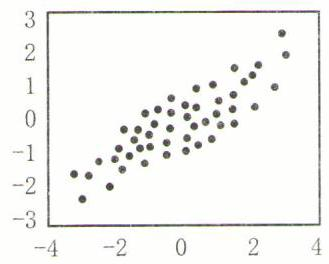
\includegraphics[width=0.2\textwidth]{bodyxb/src/bo_d20aucref24c73anc48g_276_262_736_329_264_0.jpg}
\end{center}


(A)

\begin{center}
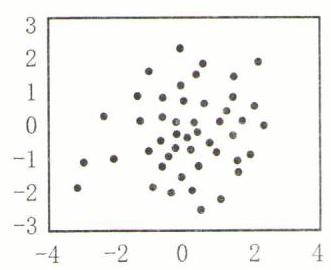
\includegraphics[width=0.2\textwidth]{bodyxb/src/bo_d20aucref24c73anc48g_276_262_1045_331_270_0.jpg}
\end{center}


(C)

\begin{center}
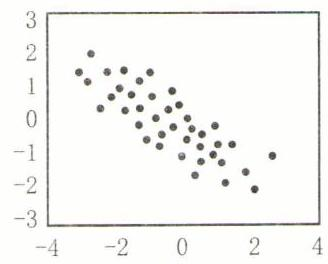
\includegraphics[width=0.2\textwidth]{bodyxb/src/bo_d20aucref24c73anc48g_276_893_733_328_264_0.jpg}
\end{center}


(B)

\begin{center}
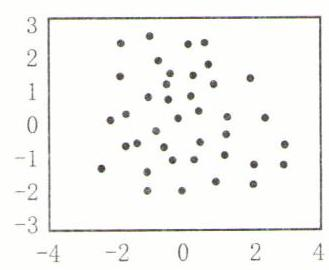
\includegraphics[width=0.2\textwidth]{bodyxb/src/bo_d20aucref24c73anc48g_276_893_1042_329_270_0.jpg}
\end{center}


(D)

111. 北极冰融是近年来最引人注目的气候变化现象之一,白色冰面融化变成颜色相对较暗的海冰, 被称为 ”北极变暗” 现象. 21 世纪以来, 北极的气温变化是全球平均水平的 2 倍, 被称为 “北极放大” 现象. 如图为北极年平均海冰面积 $\left( {{10}^{6}{\mathrm{{km}}}^{2}}\right)$ 与年平均 ${\mathrm{{CO}}}_{2}\left( \mathrm{{ppm}}\right)$ 浓度图. 下列说法正确的是(   )

\begin{center}
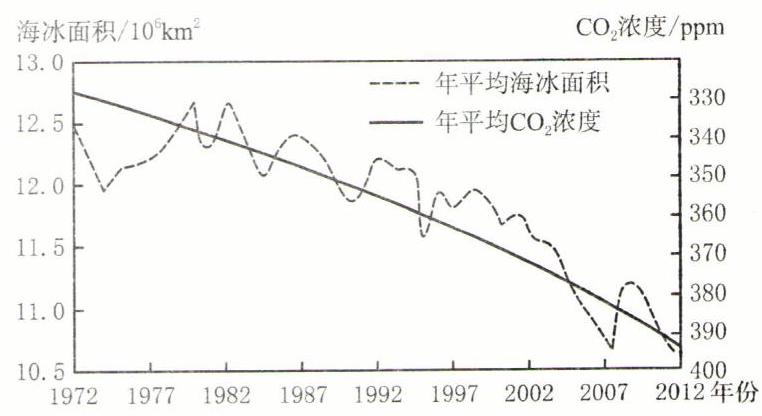
\includegraphics[width=0.6\textwidth]{bodyxb/src/bo_d20aucref24c73anc48g_276_777_1357_762_416_0.jpg}
\end{center}


(第 111 题)

(A) 北极年平均海冰面积逐年减少.

(B)北极年平均海冰面积减少速度不断加快.

(C)北极年平均海冰面积与年平均二氧化碳浓度大体呈负相关.

(D) 北极年平均海冰面积与年平均二氧化碳浓度大体呈正相关.

112. 有以下几组(x, y)的统计数据: $\left( {1,1}\right) ,\left( {2,{1.5}}\right) ,\left( {3,3}\right) ,\left( {4,{2.5}}\right) ,\left( {5,7}\right)$ . 要使剩下的数据线性相关程度更高, 应去掉的一组数据是 (   )

(A)(2,1.5). (B)(3,3). (C)(4,2.5). (D)(5,7).

113. 在研究某高中高三年级学生的性别与是否喜欢某学科的关系时,共调查了 $N$ 个学生 $(N$  $= {100m},m$ 为正整数),其中男女学生各半,男生中 ${60}\%$ 表示喜欢该学科,其余表示不喜欢；女生中 40\%表示喜欢该学科,其余表示不喜欢. 若有 99.9\% 的把握认为性别与是否喜欢该学科有关,则可以推测 $N$ 的最小值为 (   )

\begin{center}
\adjustbox{width=\textwidth}{
\begin{tabular}{|c|c|c|c|}
\hline
$P\left( {{\chi }^{2} \geq  k}\right)$ & 0.050 & 0.010 & 0.001 \\
\cline{1-4}
$k$ & 3.841 & 6.635 & 10.828 \\
\cline{1-4}
\hline
\end{tabular}
}
\end{center}

(A) 400. (B) 300. (C) 200. (D) 100.

114. 经研究表明健康的饮食和科学的运动能够有效减少低密度脂蛋白浓度. 为了调查某地青年人的低密度脂蛋白浓度是否与肥胖有关,随机调查了该地 100 名青年,得到 $2 \times  2$ 列联表如下:

\begin{center}
\adjustbox{width=\textwidth}{
\begin{tabular}{|c|c|c|c|}
\hline
\phantom{X} & 肥胖 & 不肥胖 & 总计 \\
\cline{1-4}
低密度脂蛋白不高于3.1 mmol/L & 10 & 65 & 75 \\
\cline{1-4}
低密度脂蛋白高于3.1 mmol/L & 10 & 15 & 25 \\
\cline{1-4}
总计 & 20 & 80 & 100 \\
\cline{1-4}
\hline
\end{tabular}
}
\end{center}

由此得出的正确结论是(   )

(A) 在犯错误的概率不超过 0.5\%的前提下, 认为 “该地青年人的低密度脂蛋白浓度与肥胖有关”.

(B) 在犯错误的概率不超过 0.5\%的前提下, 认为 “该地青年人的低密度脂蛋白浓度与肥胖无关”.

(C) 在犯错误的概率不超过 0.1\%的前提下, 认为 “该地青年人的低密度脂蛋白浓度与肥胖有关”.

(D) 在犯错误的概率不超过 0.1\%的前提下, 认为 “该地青年人的低密度脂蛋白浓度与肥胖无关”.

附:

\begin{center}
\adjustbox{width=\textwidth}{
\begin{tabular}{|c|c|c|c|c|c|}
\hline
$\alpha$ & 0.1 & 0.05 & 0.01 & 0.005 & 0.001 \\
\cline{1-6}
${x}_{a}$ & 2.706 & 3.841 & 6.635 & 7.879 & 10.828 \\
\cline{1-6}
\hline
\end{tabular}
}
\end{center}

115. 下表是某小卖部 6 天卖出热茶的杯数与当天气温的对比表:

\begin{center}
\adjustbox{width=\textwidth}{
\begin{tabular}{|c|c|c|c|c|c|c|}
\hline
气温 $x/{}^{ \circ  }\mathrm{C}$ & 26 & 18 & 13 & 10 & 4 & -1 \\
\cline{1-7}
杯数 $y$ /杯 & 20 & 24 & 34 & 38 & 50 & 64 \\
\cline{1-7}
\hline
\end{tabular}
}
\end{center}

\begin{center}
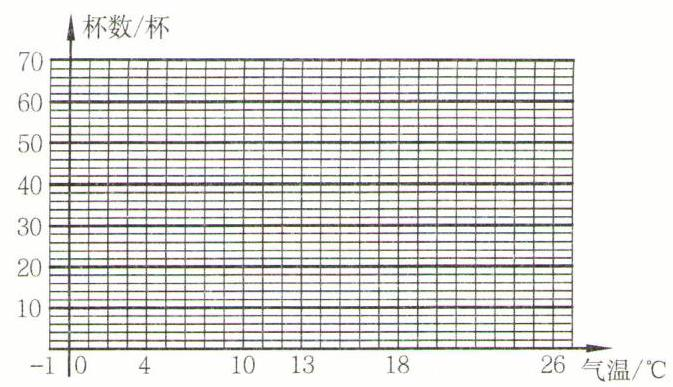
\includegraphics[width=0.5\textwidth]{bodyxb/src/bo_d20aucref24c73anc48g_278_513_138_673_387_0.jpg}
\end{center}


根据表中数据绘制散点图,计算相关系数并判断热茶销量与气温的相关程度.

116. 如图是我国 2018 年至 2024 年年生活垃圾无害化处理量 (单位: 亿吨) 的折线图.

\begin{center}
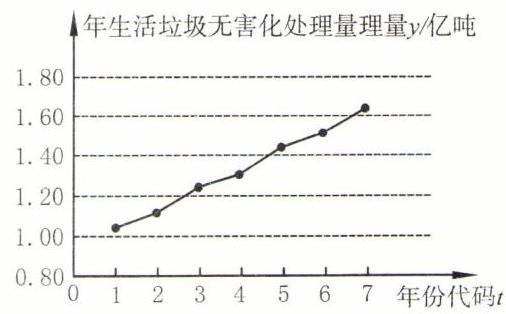
\includegraphics[width=0.4\textwidth]{bodyxb/src/bo_d20aucref24c73anc48g_278_1021_582_506_314_0.jpg}
\end{center}


(第 116 题)

已知: $\mathop{\sum }\limits_{{i = 1}}^{7}{y}_{i} = {9.32},\mathop{\sum }\limits_{{i = 1}}^{7}{t}_{i}{y}_{i} = {40.17},\sqrt{\mathop{\sum }\limits_{{i = 1}}^{7}{\left( {y}_{i} - \bar{y}\right) }^{2}} = {0.55}$ .

注:年份代码 1\~7 分别对应年份 2018\~2024.

问: 是否可以用线性回归模型拟合 $y$ 与 $t$ 的关系? 请用相关系数加以说明.

117. 某大学生去工厂实习,实习结束时从他制作的某种零件中随机选取了 10 个样品,并测量每个零件的横截面积 $\left( {\text{ 单位: }\mathrm{m}{\mathrm{m}}^{2}}\right)$ 和耗材量 $\left( {\text{ 单位: }\mathrm{m}{\mathrm{m}}^{3}}\right)$ ,得到如下数据:

\begin{center}
\adjustbox{width=\textwidth}{
\begin{tabular}{|c|c|c|c|c|c|c|c|c|c|c|c|}
\hline
样本号 ${\lambda }_{i}$ & 1 & 2 & 3 & 4 & 5 & 6 & 7 & 8 & 9 & 10 & 总和 \\
\cline{1-12}
零件的横截面积 ${x}_{i}$ & 0.03 & 0.05 & 0.04 & 0.07 & 0.07 & 0.04 & 0.05 & 0.06 & 0.06 & 0.05 & 0.52 \\
\cline{1-12}
耗材量 ${y}_{i}$ & 0.24 & 0.40 & 0.23 & 0.55 & 0.50 & 0.34 & 0.35 & 0.45 & 0.43 & 0.41 & 3.9 \\
\cline{1-12}
\hline
\end{tabular}
}
\end{center}

经计算得 $\mathop{\sum }\limits_{{i = 1}}^{{10}}{x}_{i}{y}_{i} = {0.2143},\left( {\mathop{\sum }\limits_{{i = 1}}^{{10}}{x}_{i}^{2} - {10}{\bar{x}}^{2}}\right) \left( {\mathop{\sum }\limits_{{i = 1}}^{{10}}{y}_{i}^{2} - {10}{\bar{y}}^{2}}\right)  = {1.49136} \times  {10}^{-4}$ .

(1)估算该学生制作的这种零件平均每个零件的横截面积以及平均一个零件的耗材量；

(2)求该学生制作的这种零件的横截面积和耗材量的样本相关系数(精确到 0.01).

118. 某地区为响应“节能减排,低碳生活”的号召,开展一系列的措施控制碳排放. 环保部门收集到近 5 年内新增碳排放数量,如下表所示,其中 $x$ 为年份代号, $y$ (单位: 万吨) 代表新增碳排放量.

\begin{center}
\adjustbox{width=\textwidth}{
\begin{tabular}{|c|c|c|c|c|c|}
\hline
年份 & 2020 & 2021 & 2022 & 2023 & 2024 \\
\cline{1-6}
年份代号 $x$ & 1 & 2 & 3 & 4 & 5 \\
\cline{1-6}
新增碳排放量 $y$ /万吨 & 6. 1 & 5.2 & 4. 9 & 4 & 3.8 \\
\cline{1-6}
\hline
\end{tabular}
}
\end{center}

(1)请计算相关系数 $r$ ,并推断 $x$ 与 $y$ 之间是否具有较强的线性相关性？(若 $\left| r\right|  > {0.75}$ , 则可以认为 $x,y$ 之间线性相关程度较高);

(2)求 $y$ 关于 $x$ 的线性回归方程,并据此估计该地区 2025 年的新增碳排放量.

119. 随着近年来生活质量的提高,饮食结构改变,生活压力增加,中青年人也逐渐成为动脉粥样硬化性心血管疾病(ASCVD)的高危人群. 血脂异常是 ASCVD 的重要危险因素之一, 有效控制血脂异常, 对防治 ASCVD 具有重要意义. 某公司计划研究一种新的降脂单抗药物, 药物研发时, 需要对志愿者进行药效实验. 该公司统计了 800 名不同年龄的志愿者达

到预期效果所需的疗程数, 得到如下频数分布表:

\begin{center}
\adjustbox{width=\textwidth}{
\begin{tabular}{|c|c|c|c|c|}
\hline
年龄 & $\lbrack {15},{25})$ & $\lbrack {25},{35})$ & $\lbrack {35},{45})$ & $\left\lbrack  {{45},{55}}\right\rbrack$ \\
\cline{1-5}
1 次 & 40 & 50 & 50 & 90 \\
\cline{1-5}
$2 \sim  4$ 次 & 100 & 60 & 100 & 50 \\
\cline{1-5}
5\~10 次 & 61 & 75 & 55 & 43 \\
\cline{1-5}
10 次以上 & 7 & 7 & 5 & 7 \\
\cline{1-5}
\hline
\end{tabular}
}
\end{center}

把年龄在 $\lbrack {15},{35})$ 内的人称为青年,年龄在 $\left\lbrack  {{35},{55}}\right\rbrack$ 内的人称为中年,疗程数低于 5 次的为效果明显, 不低于 5 次的为效果不明显.

(1)补全下面的 $2 \times  2$ 列联表；

\begin{center}
\adjustbox{width=\textwidth}{
\begin{tabular}{|c|c|c|c|}
\hline
\multirow{2}{*}{效果} & \multicolumn{2}{|c|}{年龄} & \multirow{2}{*}{合计} \\
\cline{2-3}
 & 青年 & 中年 &  \\
\cline{1-4}
效果不明显 & \phantom{X} & \phantom{X} & \phantom{X} \\
\cline{1-4}
效果明显 & \phantom{X} & \phantom{X} & \phantom{X} \\
\cline{1-4}
合计 & \phantom{X} & \phantom{X} & \phantom{X} \\
\cline{1-4}
\hline
\end{tabular}
}
\end{center}

(2)判断以 35 岁为分界点,根据小概率值 $\alpha  = {0.01}$ 的独立性检验,能否认为治疗效果与年龄有关.

附:

\begin{center}
\adjustbox{width=\textwidth}{
\begin{tabular}{|c|c|c|c|c|}
\hline
$\alpha$ & 0.10 & 0.05 & 0.01 & 0.001 \\
\cline{1-5}
${\chi }_{a}$ & 2.706 & 3.841 & 6.635 & 10.828 \\
\cline{1-5}
\hline
\end{tabular}
}
\end{center}

(B)

120. 对四组数据进行统计, 获得以下散点图, 关于其样本相关系数的比较, 下列结论正确的是(   )

\begin{center}
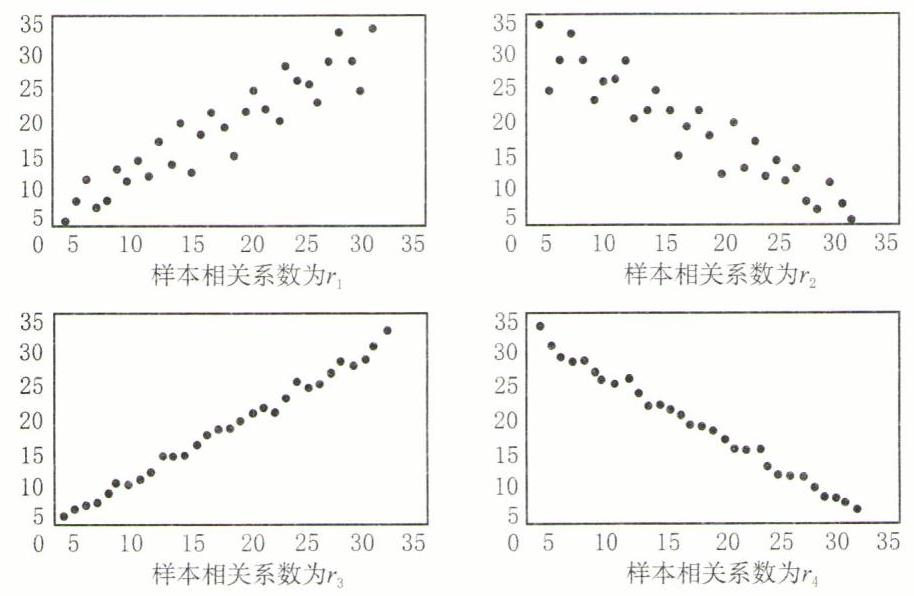
\includegraphics[width=0.7\textwidth]{bodyxb/src/bo_d20aucref24c73anc48g_279_325_1433_914_596_0.jpg}
\end{center}


(第 120 题)

(A) ${r}_{2} < {r}_{4} < 0 < {r}_{3} < {r}_{1}$ . (B) ${r}_{4} < {r}_{2} < 0 < {r}_{1} < {r}_{3}$ .

(C) ${r}_{4} < {r}_{2} < 0 < {r}_{3} < {r}_{1}$ . (D) ${r}_{2} < {r}_{4} < 0 < {r}_{1} < {r}_{3}$ .

121. 变量 $X$ 与 $Y$ 相对应的一组数据为 $\left( {{10},1}\right) ,\left( {{11.3},2}\right) ,\left( {{11.8},3}\right) ,\left( {{12.5},4}\right) ,\left( {13.5}\right)$ ; 变量 $U$ 与 $V$ 相对应的一组数据为 $\left( {{10},5}\right) ,\left( {{11.3},4}\right) ,\left( {{11.8},3}\right) ,\left( {{12.5},2}\right) ,\left( {{13},1}\right) .{r}_{1}$ 表示变量 $Y$ 与 $X$ 之间的线性相关系数, ${r}_{2}$ 表示变量 $V$ 与 $U$ 之间的线性相关系数,则 (   )

(A) ${r}_{2} < {r}_{1} < 0$ . (B) $0 < {r}_{2} < {r}_{1}$ .

(C) ${r}_{2} < 0 < {r}_{1}$ . (D) ${r}_{2} = {r}_{1}$ .

122. 通过随机抽样, 我们绘制了如图所示的某种商品每千克价格 (单位: 百元) 与该商品消费者年需求量 (单位:千克)的散点图. 若去掉图中右下方的点 $A$ 后,下列说法正确的是(   )

\begin{center}
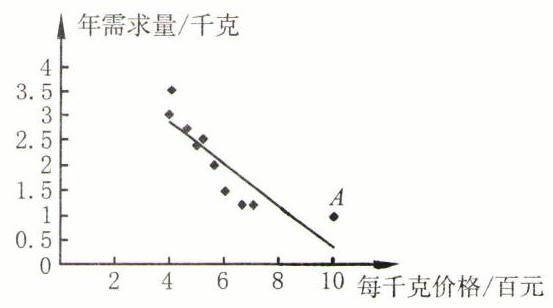
\includegraphics[width=0.4\textwidth]{bodyxb/src/bo_d20aucref24c73anc48g_280_988_413_553_308_0.jpg}
\end{center}


(第 122 题)

(A) “每千克价格”与“年需求量”这两个变量由负相关变为正相关.

(B) “每千克价格”与“年需求量”这两个变量的线性相关程度不变.

(C) “每千克价格”与“年需求量”这两个变量的线性相关系数变大.

(D) “每千克价格”与“年需求量”这两个变量的线性相关系数变小.

123. 通过随机询问相同数量的不同性别大学生在购买食物时是否看营养说明,得知有 $\dfrac{1}{5}$ 的男大学生选择 “不看”,有 $\dfrac{2}{5}$ 的女大学生选择 “不看”,若有 99.9\% 的把握认为性别与是否看营养说明之间有关,则调查的总人数至少为(   )

(A) 225 人. (B) 227 人. (C) 228 人. (D) 230 人.

附:

\begin{center}
\adjustbox{width=\textwidth}{
\begin{tabular}{|c|c|c|c|c|c|}
\hline
$\alpha$ & 0.1 & 0.05 & 0.01 & 0.005 & 0.001 \\
\cline{1-6}
${\chi }_{a}$ & 2.706 & 3.841 & 6.635 & 7.879 & 10.828 \\
\cline{1-6}
\hline
\end{tabular}
}
\end{center}

124. 某数学兴趣小组在探究姜撞奶随着时间变化的降温及凝固情况的数学建模活动中,将时间 (min) 与温度 $\left( {{}^{ \circ  }\mathrm{C}}\right)$ 的关系用模型 $y = {c}_{1}{\mathrm{e}}^{{c}_{2}x}$ (其中 $\mathrm{e}$ 为自然对数的底数) 拟合. 令 $z =$  $\ln y$ ,经变换后可以得到如下数据:

\begin{center}
\adjustbox{width=\textwidth}{
\begin{tabular}{|c|c|c|c|c|c|}
\hline
$x$ & 2 & 2.5 & 3 & 3.5 & 4 \\
\cline{1-6}
$z$ & 4.04 & 4.01 & 3. 98 & 3. 96 & 3. 91 \\
\cline{1-6}
\hline
\end{tabular}
}
\end{center}

由上表可得线性回归方程 $z =  - {0.062x} + t$ ,则 ${c}_{1}$ 等于(   )

(A) -0.062 . (B) ${\mathrm{e}}^{-{0.062}}$ . (C) 4.166. (D) ${\mathrm{e}}^{4.166}$ .

125. 为探究药物 $A$ 对疾病 $B$ 的治疗效果,将 40 名患者平均分为两组,分别为对照组 (未服药) 和实验组 (服药).

(1)任选两名患者,求已知其中一名患者在实验组的条件下,另一名患者在对照组的概率;

(2)测得 40 名患者血液中的某个指标数据如下(单位:mg):

对照组:

$\begin{array}{llllllllll} {18.3} & {19.4} & {20.1} & {21.4} & {22.6} & {23.4} & {24.4} & {24.9} & {25.3} & {25.9} \end{array}$

$\begin{array}{llllllllll} {26.2} & {26.7} & {26.8} & {26.8} & {26.9} & {27.3} & {27.4} & {27.5} & {27.6} & {35.3} \end{array}$

实验组:

$\begin{array}{llllllllll} {4.4} & {5.3} & {5.8} & {6.9} & {7.3} & {8.1} & {8.4} & {9.0} & {10.4} & {13.2} \end{array}$

$\begin{array}{llllllllll} {13.4} & {16.3} & {18.2} & {19.3} & {23.6} & {24.1} & {24.5} & {24.7} & {25.2} & {25.3} \end{array}$

①求这 40 名患者血液中的该指标数据的中位数 $m$ ,并完成下面的 $2 \times  2$ 列联表:

\begin{center}
\adjustbox{width=\textwidth}{
\begin{tabular}{|c|c|c|c|}
\hline
\multirow{2}{*}{药物 $A$} & \multicolumn{2}{|c|}{疾病 $B$} & \multirow{2}{*}{合计} \\
\cline{2-3}
 & 指标数据 $< m$ & 指标数据 $\geq  m$ &  \\
\cline{1-4}
对照组 & \phantom{X} & \phantom{X} & \phantom{X} \\
\cline{1-4}
实验组 & \phantom{X} & \phantom{X} & \phantom{X} \\
\cline{1-4}
合计 & \phantom{X} & \phantom{X} & \phantom{X} \\
\cline{1-4}
\hline
\end{tabular}
}
\end{center}

②依据小概率值 $\alpha  = {0.01}$ 的独立性检验,能否认为药物 $A$ 对治疗疾病 $B$ 有效？

附: 回归直线的斜率和截距的最小二乘估计公式分别为

$\widehat{a} = \dfrac{\mathop{\sum }\limits_{{i = 1}}^{n}\left( {{x}_{i} - \bar{x}}\right) \left( {{y}_{i} - \bar{y}}\right) }{\mathop{\sum }\limits_{{i = 1}}^{n}{\left( {x}_{i} - \bar{x}\right) }^{2}} = \dfrac{\mathop{\sum }\limits_{{i = 1}}^{n}{x}_{i}{y}_{i} - n\bar{x}\bar{y}}{\mathop{\sum }\limits_{{i = 1}}^{n}{x}_{i}^{2} - n{\bar{x}}^{2}},\widehat{b} = \bar{y} - \widehat{a}\bar{x}$

\begin{center}
\adjustbox{width=\textwidth}{
\begin{tabular}{|c|c|c|c|c|c|}
\hline
$\alpha$ & 0.10 & 0.05 & 0.010 & 0.005 & 0.001 \\
\cline{1-6}
${\chi }_{a}$ & 2.706 & 3.841 & 6.635 & 7.879 & 10.828 \\
\cline{1-6}
\hline
\end{tabular}
}
\end{center}

126. 某网络购物平台专营店统计了某年 2 月 15 日至 19 日这 5 天在该店购物的人数 $y$ 的数据如下:

\begin{center}
\adjustbox{width=\textwidth}{
\begin{tabular}{|c|c|c|c|c|c|}
\hline
日期 & 2 月 15 日 & 2 月 16 日 & 2 月 17 日 & 2 月 18 日 & 2 月 19 日 \\
\cline{1-6}
日期代号 $x$ & 1 & 2 & 3 & 4 & 5 \\
\cline{1-6}
购物人数 $y$ & 77 & 84 & 93 & 96 & 100 \\
\cline{1-6}
\hline
\end{tabular}
}
\end{center}

(1)根据表中数据,建立 $y$ 关于 $x$ 的一元线性回归模型,并根据该回归模型预测当年 2 月 21 日在该店购物的人数(人数用四舍五入法取整数)；

(2)为了了解参加网购人群的年龄分布,该店随机抽取了 200 人进行问卷调查,并得到如下不完整的 $2 \times  2$ 列联表:

\begin{center}
\adjustbox{width=\textwidth}{
\begin{tabular}{|c|c|c|c|}
\hline
年龄 & 不低于 40 岁 & 低于 40 岁 & 合计 \\
\cline{1-4}
参与过网上购物 & 30 & \phantom{X} & 150 \\
\cline{1-4}
未参与过网上购物 & \phantom{X} & 30 & \phantom{X} \\
\cline{1-4}
合计 & \phantom{X} & \phantom{X} & 200 \\
\cline{1-4}
\hline
\end{tabular}
}
\end{center}

将列联表补充完整,并依据表中数据及小概率值 $\alpha  = {0.005}$ 的独立性检验,能否认为 “参与网上购物”与“年龄”有关. 附: 回归直线的斜率和截距的最小二乘估计公式分别为

$\widehat{a} = \dfrac{\mathop{\sum }\limits_{{i = 1}}^{n}\left( {{x}_{i} - \bar{x}}\right) \left( {{y}_{i} - \bar{y}}\right) }{\mathop{\sum }\limits_{{i = 1}}^{n}{\left( {x}_{i} - \bar{x}\right) }^{2}} = \dfrac{\mathop{\sum }\limits_{{i = 1}}^{n}{x}_{i}{y}_{i} - n\bar{x}\bar{y}}{\mathop{\sum }\limits_{{i = 1}}^{n}{x}_{i}^{2} - n{\bar{x}}^{2}},\widehat{b} = \bar{y} - \widehat{a}\bar{x}$

\begin{center}
\adjustbox{width=\textwidth}{
\begin{tabular}{|c|c|c|c|c|c|}
\hline
$\alpha$ & 0.10 & 0.05 & 0.010 & 0.005 & 0.001 \\
\cline{1-6}
${\chi }_{a}$ & 2.706 & 3.841 & 6.635 & 7.879 & 10.828 \\
\cline{1-6}
\hline
\end{tabular}
}
\end{center}

127. 我国风云系列卫星可以监测气象和国土资源情况. 某地区水文研究人员为了了解汛期人工测雨量 $x$ (单位: $\mathrm{{dm}}$ )与遥测雨量 $y$ (单位: $\mathrm{{dm}}$ )的关系,统计得到该地区 10 组雨量数据如下:

\begin{center}
\adjustbox{width=\textwidth}{
\begin{tabular}{|c|c|c|c|c|c|c|c|c|c|c|}
\hline
样本号 $i$ & 1 & 2 & 3 & 4 & 5 & 6 & 7 & 8 & 9 & 10 \\
\cline{1-11}
人工测雨量 ${x}_{i}$ & 5.38 & 7. 99 & 6.37 & 6.71 & 7.53 & 5.53 & 4. 18 & 4.04 & 6.02 & 4.23 \\
\cline{1-11}
遥测雨量 ${y}_{i}$ & 5.43 & 8.07 & 6.57 & 6. 14 & 7.95 & 5.56 & 4. 27 & 4. 15 & 6.04 & 4. 49 \\
\cline{1-11}
$\left| {{x}_{i} - {y}_{i}}\right|$ & 0.05 & 0.08 & 0.2 & 0.57 & 0.42 & 0.03 & 0.09 & 0.11 & 0.02 & 0.26 \\
\cline{1-11}
\hline
\end{tabular}
}
\end{center}

计算得 $\mathop{\sum }\limits_{{i = 1}}^{{10}}{x}_{i}^{2} = {353.6},\mathop{\sum }\limits_{{i = 1}}^{{10}}{y}_{i}^{2} = {361.7},\mathop{\sum }\limits_{{i = 1}}^{{10}}{x}_{i}{y}_{i} = {357.3},{\bar{x}}^{2} \approx  {33.62},{\bar{y}}^{2} \approx  {34.42},\bar{x}\bar{y} \approx  {34.02}$ .

(1)求该地区汛期遥测雨量 $y$ 与人工测雨量 $x$ 的样本相关系数 (精确到 0.01 ),并判断它们是否具有线性相关关系;

(2)规定:数组 $\left( {{x}_{i},{y}_{i}}\right)$ 满足 $\left| {{x}_{i} - {y}_{i}}\right|  < {0.1}$ 为“ $\mathrm{I}$ 类误差”；满足 ${0.1} \leq  \left| {{x}_{i} - {y}_{i}}\right|  < {0.3}$ 为 “ II 类误差”；满足 $\left| {{x}_{i} - {y}_{i}}\right|  \geq  {0.3}$ 为 “ III 类误差”. 为进一步研究,研究人员从 “ I 类误差”“II类误差”中随机抽取 3 组数据与“III类误差”数据进行对比, 记抽到“I 类误差” 的数据的组数为 $X$ ,求 $X$ 的概率分布与数学期望.

附: 相关系数 $r = \dfrac{\mathop{\sum }\limits_{{i = 1}}^{n}\left( {{x}_{i} - \bar{x}}\right) \left( {{y}_{i} - \bar{y}}\right) }{\sqrt{\mathop{\sum }\limits_{{i = 1}}^{n}{\left( {x}_{i} - \bar{x}\right) }^{2}\mathop{\sum }\limits_{{i = 1}}^{n}{\left( {y}_{i} - \bar{y}\right) }^{2}}}$

128. 环境监测部门为调研汽车流量对空气质量的影响,在某监测点统计每日过往的汽车流量 $x$ (单位:辆)和空气中的 PM2.5 的平均浓度 $y$ (单位: $\mu \mathrm{g}/{\mathrm{m}}^{3}$ ). 调研人员采集了 50 天的数据,制作了关于 $\left( {{x}_{i},{y}_{i}}\right) \left( {i = 1,2,3,\cdots ,{50}}\right)$ 的散点图,并用直线 $x = {1500}$ 与 $y = {100}$ 将散点图分成如图所示的四个区域 $\mathrm{I},\mathrm{{II}},\mathrm{{III}},\mathrm{{IV}}$ ,落入对应区域的样本点的个数依次为6,20,16,8.

\begin{center}
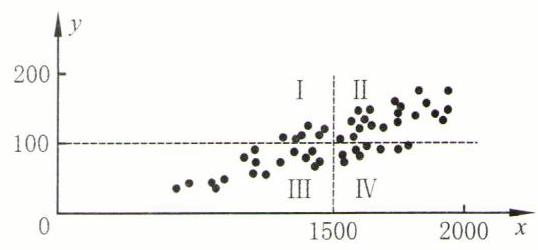
\includegraphics[width=0.4\textwidth]{bodyxb/src/bo_d20aucref24c73anc48g_282_1015_1445_538_250_0.jpg}
\end{center}


(1)完成下面的 $2 \times  2$ 列联表,并判断至少有多大把握认为 “PM2. 5 平均浓度不小于 ${100\mu }\mathrm{g}/{\mathrm{m}}^{3}$ ” 与 “汽车日流量不少于 1500 辆” 有关；

\begin{center}
\adjustbox{width=\textwidth}{
\begin{tabular}{|c|c|c|c|}
\hline
\phantom{X} & 汽车日流量 $x < 1{500}$ & 汽车日流量 $x \geq  {1500}$ & 合计 \\
\cline{1-4}
PM2. 5 的平均浓度 $y < {100}$ & \phantom{X} & \phantom{X} & \phantom{X} \\
\cline{1-4}
PM2.5 的平均浓度 $y \geq  {100}$ & \phantom{X} & \phantom{X} & \phantom{X} \\
\cline{1-4}
合计 & \phantom{X} & \phantom{X} & \phantom{X} \\
\cline{1-4}
\hline
\end{tabular}
}
\end{center}

(2)经计算得到回归方程为 $y = {0.12x} - {73.36}$ ,且这 50 天的汽车日流量 $x$ 的标准差为 252, PM2.5 的平均浓度 $y$ 的标准差为 36,求相关系数 $r$ .

附:

\begin{center}
\adjustbox{width=\textwidth}{
\begin{tabular}{|c|c|c|c|c|c|}
\hline
$\alpha$ & 0.10 & 0.05 & 0.010 & 0.005 & 0.001 \\
\cline{1-6}
${\chi }_{a}$ & 2.706 & 3.841 & 6.635 & 7.879 & 10.828 \\
\cline{1-6}
\hline
\end{tabular}
}
\end{center}

回归方程 $y = \widehat{a}x + \widehat{b}$ ,其中 $\widehat{a} = \dfrac{\mathop{\sum }\limits_{{i = 1}}^{n}\left( {{x}_{i} - \bar{x}}\right) \left( {{y}_{i} - \bar{y}}\right) }{\mathop{\sum }\limits_{{i = 1}}^{n}{\left( {x}_{i} - \bar{x}\right) }^{2}}$ .

相关系数 $r = \dfrac{\mathop{\sum }\limits_{{i = 1}}^{n}\left( {{x}_{i} - \bar{x}}\right) \left( {{y}_{i} - \bar{y}}\right) }{\sqrt{\mathop{\sum }\limits_{{i = 1}}^{n}{\left( {x}_{i} - \bar{x}\right) }^{2}\mathop{\sum }\limits_{{i = 1}}^{n}{\left( {y}_{i} - \bar{y}\right) }^{2}}}$ .

129. 在彩色显像中,根据以往的经验,形成染料的光学密度 $y$ 与析出银的光学密度 $x$ 之间存在关系式 $y = a{\mathrm{e}}^{-\dfrac{b}{x}}\left( {b > 0}\right)$ . 现对 $y$ 与 $x$ 同时做 10 次观测,获得数据如下,试根据表中数据,求出 $a$ 与 $b$ 的估计值.

\begin{center}
\adjustbox{width=\textwidth}{
\begin{tabular}{|c|c|c|c|c|c|c|c|c|c|c|}
\hline
编号 & 1 & 2 & 3 & 4 & 5 & 6 & 7 & 8 & 9 & 10 \\
\cline{1-11}
$x$ & 0.05 & 0.06 & 0.07 & 0.10 & 0.14 & 0.20 & 0.25 & 0.31 & 0.38 & 0.43 \\
\cline{1-11}
$y$ & 0.10 & 0.14 & 0.23 & 0.37 & 0.59 & 0.79 & 1.00 & 1. 12 & 1.19 & 1.25 \\
\cline{1-11}
\hline
\end{tabular}
}
\end{center}